\documentclass{report}

\usepackage[spanish]{babel}  
\usepackage{graphicx}
\usepackage{amsmath}
\usepackage{cite}
\usepackage{hyperref}
\usepackage{caption}
\usepackage{float}
\usepackage{listings}
\usepackage[utf8]{inputenc}  % Soporte para caracteres en español
\usepackage{graphicx}        % Para incluir imágenes si lo deseas
\usepackage{titling}   

\renewcommand{\topfraction}{0.9} % Máximo 90% de la página para figuras en la parte superior
\renewcommand{\textfraction}{0.1} % Mínimo 10% de texto en cada página
\renewcommand{\floatpagefraction}{0.8} % No crear una página solo para figuras hasta llenar el 80%

\begin{document}

%----------------------------------------------------------------------
\begin{titlepage}
    \centering
    {\LARGE \textbf{Universidad de Antioquia}}\\
    {\Large Facultad de Ciencias Exactas y Naturales}\\
    {\Large Instituto de Física}\\[3cm] % Espaciado

    {\huge \textbf{Diseño e Implementación de un Sistema de Detección de Partículas Basado en GEM y FPGA SoC}}\\[2cm]

    \textbf{Autor:}\\
    {\Large Sebastián Montoya Hernández}\\[1cm]

    \textbf{Trabajo de grado para optar por el título de Físico}\\[1cm]

    \textbf{Asesor:}\\
    {\Large Profesor PhD. Johny A. Jaramillo Gallego}\\[2cm]

    {\Large Medellín, Colombia}\\
    {\Large Marzo, 2025} % Fecha automática, puedes cambiarla por una fija

\end{titlepage}
%----------------------------------------------------------------------

\tableofcontents 
%----------------------------------------------------------------------
\newpage
\section*{Introducción}  
\addcontentsline{toc}{section}{Introducción}

\noindent La exploración de los fenómenos físicos requiere de herramientas capaces de detectar, registrar y analizar las interacciones fundamentales entre la materia y la radiación. A lo largo de la historia, el desarrollo de tecnologías de detección ha sido crucial para ampliar nuestro conocimiento sobre el universo, desde el estudio de partículas subatómicas hasta aplicaciones en ciencia médica y astrofísica. En este contexto, los detectores de radiación ionizante y los sistemas de adquisición de datos (DAQ) han evolucionado como componentes esenciales en la instrumentación científica moderna, permitiendo no solo la identificación y caracterización de eventos físicos, sino también la gestión eficiente de la información obtenida en estos procesos.\\

\noindent Dentro de la amplia gama de detectores disponibles, los sistemas gaseosos han demostrado ser herramientas versátiles para la detección de partículas cargadas, debido a su alta sensibilidad y capacidad de operar en ambientes de radiación intensa. En particular, los detectores GEM (Gas Electron Multipliers) han emergido como una solución avanzada para la obtención de señales con alta resolución espacial y temporal, siendo utilizados en experimentos de física de partículas, imagenología médica y monitoreo de radiación en diversos entornos. Estos dispositivos permiten amplificar las señales generadas por la ionización de gases, proporcionando información precisa sobre trayectorias y energía de las partículas incidentes.\\

\noindent Sin embargo, la capacidad de un detector para proporcionar información útil depende no solo de su diseño, sino también de la eficiencia con la que sus señales son adquiridas y procesadas. Aquí es donde los sistemas de adquisición de datos desempeñan un papel fundamental. La instrumentación electrónica moderna ha permitido el desarrollo de DAQs altamente optimizados, capaces de capturar, digitalizar y analizar grandes volúmenes de información en tiempo real. Tecnologías como los dispositivos FPGA han potenciado esta capacidad, brindando rapidez y flexibilidad en el tratamiento de señales, aspectos clave en experimentos de alta complejidad.\\

\noindent Este trabajo se enmarca en el desarrollo y estudio experimental de un detector triple GEM, junto con la implementación de un sistema de adquisición de datos para su correcta operación y análisis. La combinación de ambas tecnologías no solo permite una mejor caracterización de los eventos detectados, sino que también fortalece la capacidad de procesamiento y optimización de la información obtenida. A través de este estudio, se busca contribuir al desarrollo de infraestructura experimental en la Universidad de Antioquia, proporcionando herramientas que pueden ser empleadas en futuras investigaciones en detección de partículas y radiación.\\

\noindent En el presente documento se abordarán, en capítulos independientes, tanto el diseño y funcionamiento de los detectores GEM como la implementación de los sistemas de adquisición de datos necesarios para su operación. Se explorarán los fundamentos físicos que rigen su desempeño, los métodos experimentales empleados para su caracterización y los resultados obtenidos en el montaje y prueba de estos sistemas, con el objetivo de ofrecer una visión integral sobre la importancia de la sinergia entre detección y procesamiento de señales en la física experimental.


\chapter{\centering {Detectores gaseosos y GEMs}}

\vspace{1cm}

\noindent Desde los primeros experimentos en física de partículas hasta las más avanzadas investigaciones en astropartículas y física médica, la detección de radiación ionizante ha sido un pilar fundamental en el desarrollo del conocimiento científico. La interacción de partículas energéticas con la materia permite obtener información crucial sobre su naturaleza y propiedades, dando lugar a la evolución de una amplia variedad de tecnologías de detección. Entre ellas, los detectores gaseosos han desempeñado un papel clave debido a su capacidad para registrar eventos de ionización en medios gaseosos con alta resolución espacial y temporal.\\

\noindent El estudio de los procesos físicos que ocurren dentro de estos detectores es esencial para comprender su funcionamiento y mejorar su desempeño. Cuando una partícula cargada atraviesa un gas, genera pares de iones y electrones que, bajo la influencia de un campo eléctrico, pueden ser recolectados y amplificados para producir señales medibles. Este principio ha dado lugar a distintos tipos de detectores gaseosos, como los contadores Geiger-Müller, las cámaras de proyección de hilos múltiples (Multi-Wire Proportional Chambers, MWPC), las cámaras de placas resistivas (Resistive Plate Chambers, RPCs) y los detectores de micropatrones. Cada uno de estos dispositivos ha sido optimizado para aplicaciones específicas, desde la detección de radiación en ambientes hostiles hasta la implementación en grandes experimentos de física de partículas.\\

\noindent En las últimas décadas, la necesidad de mejorar la resolución espacial y la capacidad de detección en altas tasas de radiación ha impulsado el desarrollo de nuevas tecnologías basadas en microestructuras. En este contexto, los detectores de microestructuras gaseosas (Micropattern Gaseous Detectors, MPGD) han surgido como una alternativa eficiente y versátil. Entre ellos, los detectores de microestructuras con multiplicación de electrones (Gas Electron Multipliers, GEMs) han demostrado ser una solución robusta para diversas aplicaciones, desde experimentos en aceleradores de partículas hasta sistemas de imagen médica y monitores de radiación en astrofísica.\\

\noindent Este trabajo se centra en el estudio y montaje experimental de un detector basado en la configuración triple GEM, desarrollado en el Grupo de Investigación en Instrumentación Científica del Instituto de Física de la Universidad de Antioquia. La construcción y caracterización de este detector representa un avance significativo en las capacidades técnicas de la universidad, el país y la región, ya que este tipo de dispositivos suelen ensamblarse en centros de investigación con infraestructura altamente especializada. Además, este desarrollo fortalece la participación del grupo en colaboraciones internacionales dentro de la física de partículas, al permitir el diseño, ensamble y validación de detectores gaseosos, así como el desarrollo de electrónica de lectura y adquisición de datos.\\

\noindent A lo largo de este documento, se presentará un marco teórico detallado que abarca los procesos de ionización en gases por interacción con partículas energéticas, los mecanismos de amplificación electrónica en estructuras sometidas a altos campos eléctricos y la evolución de los principales detectores gaseosos. Posteriormente, se describirá el montaje experimental del detector triple GEM, incluyendo los materiales y protocolos empleados en su diseño y ensamble. Finalmente, se discutirán los resultados obtenidos y su impacto en el desarrollo de tecnología de detección en el ámbito académico y experimental.\\

\newpage
\section{Marco teórico}

\noindent Los detectores gaseosos, incluidos los multiplicadores de electrones gaseosos (GEM, por sus siglas en inglés), desempeñan un papel fundamental en numerosos experimentos de física de partículas, ya que permiten la medición de partículas cargadas mediante la ionización de gases. Estos detectores son capaces de rastrear con gran precisión las trayectorias de las partículas, incluso en entornos con campos magnéticos. En comparación con los detectores de semiconductores, los detectores gaseosos suelen ser más económicos, especialmente en aplicaciones que requieren la cobertura de grandes volúmenes, y contienen menos material que pueda interferir con las partículas incidentes \cite{sauli2015gaseous}. Dado que los detectores GEM son el tema central de este trabajo, en este capítulo se analizarán tanto los principios fundamentales de la física que rigen sus interacciones y funcionamiento como algunos de los tipos de detectores de los que derivan.\\ 

\noindent En primer lugar, se explora la estadística asociada a la detección de partículas en un medio gaseoso, seguida del análisis de la interacción radiación-materia a través de la relación de poder de frenado. Utilizando un marco basado en el transporte de cargas, se estudia el funcionamiento de los detectores gaseosos como multiplicadores de carga, teniendo en cuenta el fenómeno de avalanchas de electrones como mecanismo principal. Además, se describen las características de las señales típicas esperadas a partir de estos eventos.\\

\noindent A continuación, con una base física ya establecida, se explica el funcionamiento de los detectores desde los más simples, como las cámaras de ionización, los contadores proporcionales y los detectores Geiger-Müller, hasta su evolución hacia cámaras proporcionales multi-hilos (MWPCs) y cámaras de placas resistivas (RPCs). Posteriormente, se aborda la transición hacia la miniaturización de las estructuras multiplicadoras de carga, como los detectores gaseosos de micropatrones (MPGDs), lo que culmina en los GEMs. Finalmente, se destaca una de las principales ventajas de los GEMs: la posibilidad de apilar múltiples capas, logrando importantes ganancias en la detección sin comprometer la electrónica de lectura, gracias a su capacidad para evitar descargas significativas.

\subsection{Principios físicos de los detectores gaseosos}

\noindent En términos generales, la detección de una partícula se logra mediante la deposición de una fracción o la totalidad de su energía en el medio con el que interactúa. Aunque fenómenos como la luminiscencia o la emisión de fotones de centelleo, entre otros, pueden manifestarse como resultado de la interacción entre partículas cargadas o fotones y medios gaseosos, la ionización es la interacción predominante en sistemas de baja densidad, y puede aprovecharse para generar una señal medible. En el proceso de ionización de un gas, la energía de la partícula incidente excita los electrones de las capas externas de los átomos, liberándolos y formando pares ion-electrón en su recorrido. Estos electrones iniciales pueden continuar interactuando con el medio, provocando nuevas ionizaciones y excitaciones. En materiales compuestos, los procesos secundarios también contribuyen al número total de electrones generados, ya que parte de la energía de excitación se transforma en ionización o viceversa \cite{kolanoski2020particle1}. Aunque los detectores gaseosos se centran principalmente en la captación de los electrones liberados por la radiación ionizante, la presencia de iones, estados excitados o fotones puede desencadenar fenómenos secundarios, como recombinación, transferencia de carga y efectos fotoeléctricos. En la figura \ref{fig:ionization_chamber1}, se ilustra la estructura básica de un detector gaseoso.

\begin{figure}[H]
    \centering
    \includegraphics[width=1.0\textwidth]{ionization_chamber.PNG}
    \caption{Diagrama que describe el funcionamiento básico de un detector gaseoso \cite{kolanoski2020particle2}. El medio sensible del detector, en este caso un gas, se encuentra entre dos electrodos con un voltaje aplicado. Cuando una partícula cargada atraviesa el gas, se liberan cargas que se desplazan hacia los electrodos impulsadas por el campo eléctrico. Estas cargas en movimiento generan una señal de corriente en los electrodos. En esencia, el detector actúa como un condensador que se descarga cuando el medio es ionizado. Desde el punto de vista eléctrico, se comporta como una fuente de corriente.}
    \label{fig:ionization_chamber1}
\end{figure}

\noindent Si los eventos de ionización en un gas son estudiados de manera independiente en este contexto, es posible realizar una descripción que sigue la estadística de Poisson

\begin{equation}
    \label{eq:poisson}
    P_k^n=\frac{n^k}{k!} \mathrm{e}^{-n}
\end{equation}

\noindent donde $ P_k^n$ es la probabilidad de observar $k$ eventos en un intervalo fijo, dado un promedio o tasa de eventos $n$. Por definición, se asume que los eventos son independientes: la ocurrencia de uno no afecta la probabilidad de los demás. De esta manera, la eficiencia teórica del detector, entendida como la probabilidad de tener al menos una interacción, es entonces

\begin{equation}
    \label{eq:det_eff}
    \varepsilon=1-P_0^n=1-\mathrm{e}^{-n} .
\end{equation}

\noindent Debido a que no existe una expresión simple para determinar el número de encuentros ionizantes primarios, es necesario recurrir a datos obtenidos experimentalmente o a programas de simulación especializados. Si no se tienen en cuenta procesos secundarios como la recombinación, por ejemplo, siendo $\Delta E$ la energía depositada en el medio y $W_{I}$ la energía por par íonico, la cantidad total de pares iónicos en el medio puede ser calculada como 
\begin{equation}
    \label{eq:num_ion}
    N_{T} = \frac{\Delta E}{W_{I}}. \\
\end{equation}

\noindent No obstante, este es un resultado promedio. Para entender con detalle la distribución energética en este fenómeno, es necesario acudir a un marco teórico más robusto \cite{fano1963penetration} \cite{northcliffe1963passage}. La pérdida de energía cinética de la partícula a medida que avanza por el volumen del detector es conocida como stopping power o ecuación de Bethe-Bloch y una formulación semiclásica para calcularla en un medio de grosor $\Delta x$ es: 

\begin{equation}
    \label{eq:bethe_bloch}
    \frac{\Delta E}{\Delta x}=-\rho \frac{2 K Z}{A \beta^2}\left[\ln \frac{2 m c^2 \beta^2}{I\left(1-\beta^2\right)}-\beta^2-\frac{C}{Z}-\frac{\delta}{2}\right], \quad K = \frac{2 \pi N e^{4}}{mc^{2}}
    \end{equation}

\noindent donde $\beta$ es la velocidad de la partícula, $m$ y $e$ son la masa y la carga del electrón, $Z$, $A$ y $\rho$ son el número atómico, masa atómica y la densidad del medio, $I$ es el potencial promedio de ionización del medio, el término $C/Z$ hace referencia a correcciones por apantallamiento con capas electrónicas internas y $\delta /2$ solo tiene relevancia en el régimen relativista. Para estimar las mencionadas correcciones, es necesario acudir a tablas de referencia o hallar los parámetros a partir de ajustes con datos experimentales.\\ 

\noindent Algunas consideraciones que deben ser tenidas en cuenta respecto a la ecuación de Bethe-Bloch, son su aplicabilidad a medios isotrópicos, debido a la aparición de "channeling effects" en sistemas cristalinos y las excepción de electrones y protones como partículas incidentes por su indistinguibilidad en la materia [2].\\

\noindent Teniendo en cuenta que la velocidad de la partícula ionizante es uno de los parámetros que rigue la ecuación \ref{eq:bethe_bloch}, es posible describir el comportamiento de su pérdida de energía para distintos regímenes de velocidad como ilustra la figura \ref{fig:bethe_b}.

\begin{figure}[H]
    \centering
    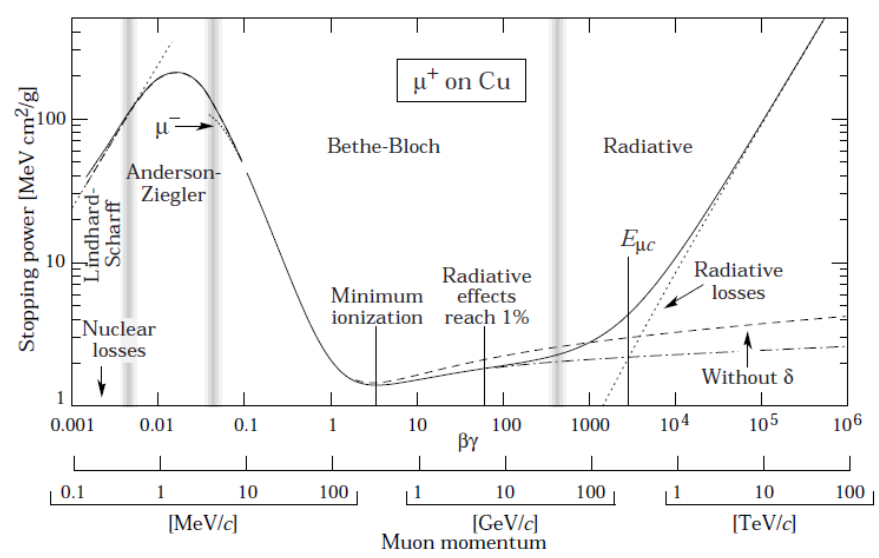
\includegraphics[width=0.8\textwidth]{bethe_bloch.PNG}
    \caption{La fórmula de Bethe-Bloch para muones positivos en cobre como función de la velocidad \cite{morisbak2010search} (mostrada entre la segunda y tercera banda gris. El resto se describe mediante otros modelos).}
    \label{fig:bethe_b}

\end{figure}

\noindent Los iones y electrones generados por procesos ionizantes en un gas pierden rápidamente su energía mediante sucesivas colisiones con las moléculas del entorno, equilibrándose con la energía térmica del medio. Al ser sometidos a campos coulombianos en el medio, las cargas se desplazan a través del gas mientras se difunden, hasta que finalmente se neutralizan, ya sea por recombinación en el propio gas o al alcanzar las paredes del recipiente. En el caso de los iones, pueden transferir su carga a otra molécula del mismo gas o a una de diferente tipo con un potencial de ionización más bajo. Los electrones, por otro lado, pueden ser neutralizados al combinarse con un ion positivo, adherirse a moléculas con afinidad electrónica o ser absorbidos por las paredes del contenedor \cite{loeb2023electrical}.\\

\noindent No obstante, a pesar de que los electrones se desplazan de forma aleatoria debido a estas interacciones con el medio, en presencia de un campo eléctrico externo, se introduce una tendencia en su desplazamiento denominado deriva electrónica. La velocidad promedio que los electrones alcanzan en su desplazamiento bajo la influencia del campo eléctrico se denomina velocidad de deriva $w^{-}$ y se define como 
\begin{equation}
    w^{-} = \mu E
\end{equation}

\noindent siendo $\mu$ la movilidad electrónica y $E$ la intensidad del campo eléctrico. Según un enfoque simple propuesto por Townsend\cite{townsend1901xvii}, la velocidad de deriva de los electrones puede expresarse mediante 
\begin{equation}
    w^{-}=k \frac{e E}{m} \tau,
\end{equation}

\noindent Aunque esta formulación resulta útil para análisis cualitativos, su aplicación práctica es limitada, ya que los valores de la velocidad de deriva $w$ y el tiempo medio entre colisiones $\tau$ dependen tanto del tipo de gas como de la intensidad del campo eléctrico. Durante su desplazamiento en presencia del campo, los electrones sufren múltiples colisiones con las moléculas, lo que provoca la difusión de la nube de carga inicial. La extensión de esta difusión depende no solo del tipo de gas, sino también de la magnitud del campo eléctrico $E$, ya que un campo más intenso permite que los electrones ganen más energía entre colisiones. De acuerdo a la teoría de transporte de carga basada en principios de mecánica estadística, es posible obtener la relación entre la movilidad electrónica $\mu$ y el coeficiente de difusión $D$, también conocida como fórmula de Nernst–Townsend \cite{loeb1947mechanism}
\begin{equation}
    \frac{D}{\mu}=\frac{\varepsilon_k}{e}
\end{equation}
\noindent donde $D$ mide la tasa de dispersión de partículas en un medio debido a movimientos aleatorios y $\varepsilon_k$ es una cantidad fenomenológica denominada energía característica, que en el caso particular de difusión térmica toma el valor de $k_{B} T$.\\

\noindent Teniendo en cuenta esto, un importante resultado de la teoría de transporte, que se deriva al considerar una distribución normal localizada de la difusión de los electrones es la expresión de su desviación estándar $\sigma_x$, que describe la extensión de la nube de electrones alrededor de un punto central a medida que se mueven a través del medio bajo la influencia del campo eléctrico aplicado \cite{sauli2015gaseous2}.
\begin{equation}
    \sigma_x=\sqrt{\frac{2 \varepsilon_k}{e} \frac{x}{E}}
\end{equation}

\noindent Esta expresión, también llamada espacio de difusión, no depende por tanto de la presión, solamente de la intensidad del campo eléctrico.\\

\noindent A medida que el campo eléctrico se incrementa, aumenta la probabilidad de colisiones ionizantes y disminuye la de excitaciones. Cada colisión ionizante crea un par electrón-ion, y el electrón primario sigue desplazándose en el gas. Si la trayectoria libre media para colisiones ionizantes es pequeña en comparación con el grosor de la capa de gas, los electrones rápidamente obtienen más energía del campo para continuar ionizando. Esto genera un crecimiento acelerado de una avalancha de electrones e iones, el mecanismo principal para amplificar señales en los contadores proporcionales de gas. Sin embargo, tras una colisión, un electrón puede transferir una cantidad de energía igual o superior a la necesaria para excitar un átomo o molécula. Luego, estos regresan al estado fundamental mediante una o varias transiciones: por ejemplo, los gases nobles emiten fotones al desexcitarse, mientras que las moléculas poliatómicas, como los hidrocarburos, disipan la energía a través de transiciones rotacionales y vibracionales sin emisión de radiación.\\

\noindent Cuando la energía de un electrón acelerado por un campo eléctrico supera el potencial de ionización de un átomo o molécula, los electrones enlazados pueden ser expulsados, dejando atrás un ion positivo. En función de la energía transferida y de la densidad de carga, pueden generarse estados de ionización múltiple. Sin embargo, en las condiciones típicas de los contadores proporcionales, donde las energías de los electrones se mantienen por debajo de unas pocas decenas de electronvoltios (eV), es más común que se formen iones con una sola carga positiva. Si los electrones primarios o secundarios no son capturados o absorbidos por las paredes del detector, continuarán moviéndose a través del gas y podrán generar nuevas ionizaciones. La trayectoria libre media para la ionización ($\lambda$) se define como la distancia promedio que recorre un electrón antes de experimentar una colisión ionizante. El inverso de esta distancia, $\alpha = \lambda ^{-1}$, se conoce como el primer coeficiente de Townsend, y representa el número de pares iónicos generados por unidad de longitud durante el desplazamiento del electrón. Este coeficiente se relaciona con la sección eficaz de ionización (probabilidad de que ocurra una ionización) mediante la expresión 
\begin{equation}
    \alpha=N \sigma_{\mathrm{i}}
\end{equation}

\noindent siendo $N$ el número de moléculas por unidad de volumen. Este mecanismo es clave para la amplificación de señales en detectores gaseosos, ya que cada colisión contribuye a la creación de más portadores de carga, permitiendo detectar eventos con mayor precisión.\\

\noindent El proceso de ionización sucesiva por colisiones permite la amplificación de carga en los contadores proporcionales. Imaginemos un electrón que se libera en una región con un campo eléctrico uniforme. Tras recorrer una trayectoria libre media $1/\alpha$, se produce un par electrón-ion. Ambos electrones continúan su desplazamiento en el gas, generando nuevos pares tras otra trayectoria libre media, y así sucesivamente. Si $n$ representa el número de electrones en una posición dada, su incremento luego de recorrer una distancia diferencial $dx$ es $dn = n \alpha dx$. Al integrar esta expresión sobre una distancia total $x$, se obtiene \cite{raether1964electron}:

\begin{equation}
n = n_0 e^{\alpha x} \quad \text{o} \quad M = \frac{n}{n_0} = e^{\alpha x},
\label{eq:multiplication}
\end{equation}

\noindent donde \(n_0\) es el número inicial de electrones y \(M\) es el factor de multiplicación o ganancia, que indica la amplificación total de carga. Esta expresión describe cómo el número de electrones crece exponencialmente con la distancia recorrida en el gas, siempre que las condiciones de ionización se mantengan constantes.\\

\noindent Para obtener una lectura precisa de la señal, se puede integrar la corriente a lo largo del tiempo, lo que permite calcular la carga total generada en el detector. La variación del voltaje registrada está relacionada con su capacitancia, y una resistencia externa se utiliza para asegurar que la carga se integre correctamente y la señal se lea con precisión. Aunque las cargas inducidas no dependen de las cargas de polarización del material, la capacitancia del sistema juega un papel crucial en la interpretación correcta de la señal medida.\\

\noindent La corriente inducida por estos electrones en avalancha aumenta con el tiempo y depende de la velocidad de deriva de los electrones y el coeficiente de Townsend. La señal rápida resultante en un contador de avalancha es una fracción de la carga total generada, destacando que al final del proceso de recolección la carga inducida total es proporcional a la carga inicial multiplicada por un factor exponencial. En la figura \ref{fig:avalanche_signal} se observan las corrientes inducidas por la contribución de los electrones e iones en la avalancha para una configuración con parámetros típicos.

\begin{figure}[H]
    \centering
    \includegraphics[width=0.8\textwidth]{avalanche_signal.png}
    \caption{Corriente inducida por avalancha en cátodos por electrones e iones. Reproducido a partir de \cite{sauli2015gaseous3}}
    \label{fig:avalanche_signal}
\end{figure}

\noindent No obstante, en el caso de una distribución extendida de carga dentro del espacio entre los electrodos, aplica el análisis que llevó a la ecuación \ref{eq:bethe_bloch}. La señal resultante depende de la densidad y distribución espacial de las cargas liberadas en el gas. En el caso particular de una ionización uniforme entre ánodo y cátodo, con una densidad \( \rho \), siendo $T$ el tiempo total de colección para los electrones en la avalanch y $w^-$ la velocidad de deriva de los electrones en avalancha, la corriente inducida por los electrones en la avalancha puede expresarse como:

\begin{equation}
i(t) = \frac{e \rho s_0}{T} \left( e^{\alpha w^- t} - \frac{t}{T} \right), \quad 0 \leq t \leq T
\end{equation}

El máximo de la señal se obtiene en un tiempo 
\begin{equation}
t_{\text{max}} = T \left( 1 - \frac{1}{\alpha s_0} \right)
\end{equation}
y tiene un valor de 
\begin{equation}
i_{\text{max}} = \frac{e \rho}{\alpha s_0} \left( e^{\alpha s_0} - 1 \right)
\end{equation}

\noindent como se muestra en la figura \ref{fig:current_avalancha}. Dado que el desarrollo de la avalancha es mucho más rápido que el tiempo de colección de los iones, la señal inducida por los iones tiene una forma muy similar (aunque no en amplitud) a la descrita previamente.

\begin{figure}[H]
    \centering
    \includegraphics[width=0.6\textwidth]{current_avalancha.PNG}
    \caption{Señal de corriente inducida en los cátodos por una trayectoria extendida bajo multiplicación de avalancha \cite{sauli2015gaseous5}.}
    \label{fig:current_avalancha}
\end{figure}

\noindent Es posible generar campos eléctricos de gran magnitud al implementar estructuras de electrodos entre las placas paralelas como un alambre (contador proporcional) \cite{montgomery1941geiger}. En la proximidad del ánodo de un contador proporcional (fig. \ref{fig:counter}), los electrones en deriva pueden ser acelerados a tal punto que pueden iniciar ionizaciones secundarias. Esto da lugar al desarrollo de una avalancha, amplificando así la carga de ionización con factores de amplificación típicos que oscilan entre \(10^4\) y \(10^6\). A partir de intensidades de campo de aproximadamente \(10-50\) kV/cm, la energía ganada entre colisiones se vuelve suficiente para causar la ionización del gas.

\begin{figure}[H]
    \centering
    \includegraphics[width=0.5\textwidth]{counter.png}
    \caption{Diagrama de un contador proporcional donde se describe sus partes principales: cámara de gas, electrodos para generación de campo eléctrico y electrónica de lectura \cite{winkler2015}.}
    \label{fig:counter}
\end{figure}

\noindent En la práctica, el régimen de amplificación se encuentra entre \(10^3\) y \(10^6\), y se puede estimar que el número de colisiones necesarias para lograr tal amplificación es de aproximadamente 13 a 20. La mayoría de los electrones tienen una trayectoria de deriva muy corta hacia el ánodo, mientras que los iones deben recorrer una distancia mayor hasta el cátodo. Esto es crucial en la formación de señales en el ánodo.\\

\noindent Sin embargo, la amplificación del gas no puede volverse arbitrariamente grande, ya que las cargas espaciales tienden a apantallar el campo cerca del ánodo, lo que se conoce como el límite de Raether \cite{raether1964electron}. Se ha observado empíricamente que el desarrollo de la avalancha alcanza una saturación en la amplificación del número de electrones primarios, en torno a \(10^8\). En este punto, el pulso de corriente en el electrodo se vuelve independiente de la ionización primaria. Contadores como el contador Geiger operan en este modo, y un aumento adicional en el voltaje puede resultar en descargas.\\

\noindent La figura \ref{fig:amplification} muestra la dependencia principal de la amplificación de gas en función del voltaje entre ánodo y cátodo para un tubo de conteo con un alambre delgado \cite{montgomery1941geiger}. 

\begin{figure}[H]
    \centering
    \includegraphics[width=0.7\textwidth]{amplification.PNG}
    \caption{Representación esquemática de la dependencia de la
    señal de salida de un tubo contador en función de la tensión ánodo-cátodo. Los valores numéricos de amplificación y tensión se utilizan a modo de ejemplo; en casos concretos dependen en gran medida de la disposición de los electrodos y del gas utilizado. }
    \label{fig:amplification}
\end{figure}

\noindent En los detectores gasesos, la elección del modo de operación depende de la aplicación prevista y diversas restricciones, como consideraciones técnicas o de seguridad. Se pueden distinguir los siguientes regímenes de amplificación \cite{kolanoski2020particle3}: 

\begin{itemize}
    \item \textbf{Región de recombinación, \(G < 1\):} En regiones de bajos campos eléctricos, los electrones primarios e iones tienden a recombinarse.
    \item \textbf{Región de cámara de ionización, \(G \approx 1\):} La señal de salida se satura sin amplificación, lo que la hace adecuada para mediciones de flujos de partículas, pero no para la detección de partículas individuales.
    \item \textbf{Región proporcional, \(G \approx 10^3 - 10^5\):} Aquí, los electrones ganan suficiente energía para producir electrones secundarios, y la carga amplificada permanece proporcional a la carga primaria en un amplio rango de voltajes.
    \item \textbf{Región proporcional, \(G \approx 10^3 - 10^5\):} Aquí, los electrones ganan suficiente energía para producir electrones secundarios, y la carga amplificada permanece proporcional a la carga primaria en un amplio rango de voltajes.
    \item \textbf{Región de proporcionalidad limitada, \(G \approx 10^5 - 10^8\):} A voltajes altos, la proporcionalidad se ve limitada por efectos de carga espacial, lo que lleva a la formación de nubes de iones cerca del ánodo.
    \item \textbf{Región de saturación y Geiger, \(G \geq 10^8\):} La señal de salida se vuelve independiente de la ionización primaria. En este modo, se "cuentan" partículas ionizantes independientemente de su tipo. La recombinación en la avalancha puede generar fotones que inician nuevas avalanchas. Sin embargo, hay un tiempo muerto significativo entre pulsos, limitando la tasa de conteo.
    \item \textbf{Región de descarga, \(G \geq 10^8 - 10^9\):} A voltajes muy altos, ocurren descargas auto-sostenidas. Es importante contar con mecanismos para la terminación controlada de estas descargas, ya que se pueden interrumpir aumentando la carga espacial o aplicando pulsos de voltaje.
\end{itemize}

\noindent Estos regímenes de operación y sus mecanismos asociados son cruciales para el funcionamiento eficiente de los detectores de gas.\\

\noindent Como se mencionó anteriormente, es posible amplificar la señal de ionización al introducir una estructura conectada a un potencial dentro de una cámara de ionización, típicamente un alambre. Los contadores proporcionales y los Geiger-Müller son los ejemplos más representativos de esta configuración. Sin embargo, las capacidades de detección pueden mejorarse significativamente en términos de resolución temporal y espacial mediante el uso de arreglos que integren múltiples alambres en diversas geometrías según la aplicación. Un ejemplo destacado de esta evolución tecnológica son las cámaras proporcionales de múltiples alambres (Multi-Wire Proportional Chambers, MWPC) (fig. \ref{fig:MWPC}).\\

\noindent Los contadores proporcionales de un solo alambre se han utilizado ampliamente para la detección y medición de pérdida de energía de radiación ionizante, pero su capacidad de localización está limitada por el tamaño físico del contador. Aunque inicialmente se creyó que estructuras con múltiples alambres no funcionarían debido a la capacitancia entre alambres paralelos sin apantallar, que dispersa la señal, Georges Charpak y colaboradores demostraron en la década de 1960 que las señales positivas inducidas en los electrodos circundantes compensan las señales negativas producidas por acoplamiento capacitivo. Esto permitió el diseño exitoso de la primera cámara proporcional de múltiples alambres \cite{charpak1968use}.\\

\noindent Este detector consiste en un conjunto de alambres delgados, paralelos y equiespaciados, colocados simétricamente entre dos planos de cátodo. Las distancias entre los alambres y los planos de cátodo suelen ser de tres a cuatro veces mayores que la separación entre alambres, aunque se han desarrollado dispositivos de brechas más delgadas. Al aplicar potenciales negativos simétricos en los cátodos y mantener los alambres a tierra, se genera un campo eléctrico que guía a los electrones hacia las regiones de alto campo cerca de los alambres, donde ocurre la multiplicación por avalancha.\\

\noindent La resolución temporal de estas cámaras depende del tiempo de colección de los electrones generados por los rastros ionizantes. El campo eléctrico alrededor de los alambres define tres regiones: en la región cercana al alambre, los electrones son recolectados rápidamente debido a la alta velocidad de deriva; en la región de menor campo entre los alambres, se produce una cola característica en la distribución temporal; y en la región más alejada, los electrones se amplifican y recolectan con un retraso proporcional al tiempo de deriva. La resolución temporal típica es de 30 ns para una cámara con separación de 2 mm entre alambres \cite{sauli1977principles}.\\

\noindent Cuando se detectan trazas no perpendiculares a la cámara, el número de alambres impactados depende de la longitud de la ventana temporal en la electrónica de detección. Si esta ventana corresponde al tiempo mínimo necesario para la eficiencia total (30 ns), solo uno o dos alambres son activados por cada traza. Sin embargo, con ventanas más largas (por ejemplo, 200 ns), el tamaño del grupo de alambres activados depende del ángulo de las trazas \cite{sauli1977principles}.\\

\noindent Charpak y colaboradores \cite{charpak1974high} también demostraron que la adición de gases electronegativos, como freón-13B1 (CF3Br), permite alcanzar una operación completamente saturada, donde la altura de los pulsos se vuelve independiente de la ionización primaria. Esta mezcla, conocida como "gas mágico" (70$\%$ argón, 29.6$\%$ isobutano y 0.4$\%$ freón), mostró una transición de un régimen casi proporcional a uno totalmente saturado. Sin embargo, la presencia de gases electronegativos también limita la eficiencia de detección, ya que la probabilidad de captura electrónica aumenta en función de la concentración del gas.\\

\noindent La amplitud elevada y el rango dinámico reducido de los pulsos saturados facilitaron el desarrollo inicial de la tecnología, simplificando los requisitos electrónicos y consolidando a las MWPC como un paso esencial en la evolución de los detectores de partículas.\\

\begin{figure}[H]
    \centering
    \includegraphics[width=0.7\textwidth]{MWPC.png}
    \caption{Diagrama básico de una Cámara proporcional multi-hilos o MWPC. Tomado de \cite{hamid2013micromegas}}
    \label{fig:MWPC}
\end{figure}

\noindent Las cámaras proporcionales de alambres múltiples (MWPC) han sido fundamentales en la detección de radiación ionizante gracias a su capacidad para proporcionar resoluciones temporales y espaciales razonables. Sin embargo, presentan limitaciones intrínsecas derivadas de la dispersión estadística en la distribución de los clústeres de ionización primaria y los efectos de difusión durante el proceso de deriva y amplificación de las cargas. Estas limitaciones impiden alcanzar resoluciones temporales óptimas, lo que motivó la búsqueda de tecnologías más avanzadas. \\

\noindent Una solución a estas limitaciones llegó con el desarrollo de las Resistive Plate Chambers (RPC), que representan una evolución significativa en la tecnología de detección. Las RPC utilizan electrodos de alta resistividad fabricados con laminados de polímero fenólico, un material económico y ampliamente disponible con resistividades volumétricas en el rango de $10^9$ a $10^{10}$ $\Omega$ cm \cite{pestov2002review}. Este diseño permite operar con eficiencias de detección cercanas al 100$\%$ y resoluciones temporales del orden de nanosegundos para partículas rápidas. El principio de funcionamiento se basa en la formación de avalanchas de ionización saturadas en gases específicos, donde el crecimiento exponencial de la avalancha es amortiguado por las cargas espaciales, evitando la propagación de descargas y mejorando la estabilidad operativa \cite{pestov2002review}. \\

\noindent La estructura básica de una RPC (véase fig. \ref{fig:RPC} ) consiste en dos placas de alta resistividad separadas por un marco aislante que mantiene la uniformidad de la distancia entre las placas. Estas están recubiertas externamente con una fina capa de grafito de moderada resistividad superficial, alrededor de 200 - 300 k$\Omega$/cuadrado, que distribuye el potencial aplicado de manera uniforme mientras permite detectar las señales inducidas por las avalanchas en tiras externas aisladas \cite{sauli2015gaseous4}. Al aplicar un voltaje adecuado, las placas alcanzan un estado de equipotencialidad, de modo que el campo eléctrico completo se aplica uniformemente a través de la capa de gas. Este diseño resulta particularmente eficiente al combinarse con mezclas de gases que absorben fotones en un amplio rango energético, lo que reduce la propagación de descargas y asegura una operación local y estable.

\begin{figure}[H]
    \centering
    \includegraphics[width=0.7\textwidth]{rpc_structure.PNG}
    \caption{Esquema de la estructura básica de un detector tipo RPC \cite{sauli2015gaseous4}.}
    \label{fig:RPC}
\end{figure}

\noindent Una de las innovaciones más destacadas en esta tecnología son las Multi-Gap Resistive Plate Chambers (MRPC), que combinan múltiples capas de gas de pequeño espesor, típicamente entre 100  y 300 $\mu$m, en una sola estructura. Este diseño permite mantener una alta eficiencia de detección mientras mejora significativamente la resolución temporal. Cada capa actúa de manera independiente, y las señales inducidas se suman en los electrodos externos, generando señales rápidas y de mayor amplitud \cite{alici2013mrpc}. \\

\noindent Una ventaja clave de las MRPC es su simplicidad en el diseño, ya que las placas internas no requieren conexión eléctrica directa; estas alcanzan su potencial de equilibrio dinámicamente cuando se aplica voltaje únicamente a las placas externas. Este enfoque simplifica la construcción de detectores de gran tamaño, donde la uniformidad del espesor del gas puede garantizarse utilizando hilos tensados entre las capas. Gracias a su excelente resolución temporal, inferior a 50 ps en algunos casos, las MRPC se han consolidado como la opción preferida para la identificación de partículas mediante mediciones de tiempo de vuelo (TOF) \cite{alici2013mrpc}. \\

\noindent Tanto las RPC como las MRPC han encontrado aplicaciones extensivas en experimentos de física de altas energías, especialmente en la detección de muones en sistemas de gran área, donde se requieren resoluciones temporales y espaciales extremas. No obstante, enfrentan ciertas limitaciones, como la modesta calidad superficial de los materiales fenólicos, que puede inducir descargas espontáneas. Este problema ha sido mitigado mediante tratamientos superficiales, como la aplicación de aceites específicos que reducen significativamente el ruido de fondo. \\

\noindent En experimentos con altos flujos de partículas, como en el LHC, se debe cuidar que la tasa de impactos por canal de lectura no sea demasiado alta. La ocupación, definida como la probabilidad promedio de registrar un impacto en un canal durante la ventana de lectura, aumenta con la tasa de impactos y reduce la información útil de cada impacto. En los detectores gaseosos, el área sensible no puede reducirse arbitrariamente debido a las limitaciones físicas en la longitud de los hilos y la necesidad de una trayectoria suficiente para la ionización.\\

\noindent Por esto, se han desarrollado detectores gaseosos con planos de lectura microestructurados, conocidos como detectores de gas de micropatrones (MPGDs), que pueden manejar altos flujos de partículas \cite{oed1988position}, manteniendo ventajas como el bajo costo. Estos detectores, que utilizan microtiras en lugar de hilos, pueden alcanzar tasas de partículas de hasta 2 MHz $/cm^{2}$ y se benefician de tecnologías tomadas de los detectores de microtiras de silicio. Además, los MPGDs son útiles no solo como detectores de partículas cargadas, sino también para medir el desplazamiento de electrones en cámaras de proyección temporal \cite{giomataris1996micromegas}.\\

\noindent Los detectores de gas microestructurados, como la cámara de gas de microtiras (MSGC), representan una mejora significativa frente a las Cámaras Proporcionales Multi-hilos (MWPC) debido a su capacidad para manejar tasas de partículas mucho más altas y ofrecer una mejor resolución espacial. Las MSGC utilizan microtiras en lugar de hilos, aplicadas mediante fotolitografía en un sustrato aislante, lo que permite una mayor densidad de partículas en el detector y minimiza las cargas espaciales que pueden alterar los campos eléctricos.\\

\noindent Entre sus ventajas, las MSGC pueden soportar tasas de partículas hasta dos órdenes de magnitud superiores a las MWPCs y alcanzar resoluciones de posición de aproximadamente 30 \textmu m, unas 10-20 veces mejor que las MWPC convencionales. También permiten la implementación modular para cubrir grandes áreas de detección sin zonas muertas y reducir la capacitancia, lo que disminuye el ruido electrónico y prolonga la vida útil del detector \cite{giomataris1996micromegas}.\\

\noindent Sin embargo, las MSGC enfrentan desafíos como las descargas incontrolables que pueden dañar los electrodos, especialmente en experimentos de alta radiación. A pesar de intentos para mitigar estos problemas, como el uso de materiales con resistencia controlada o recubrimientos especiales, su aplicación en experimentos de altas tasas de partículas ha sido limitada.\\

\subsection{GEMs}

\noindent A pesar de las limitaciones inherentes a las MSGC, el desarrollo continuo de tecnologías de detección gaseosa ha llevado a innovaciones que buscan superar los desafíos relacionados con la estabilidad operativa y la capacidad de manejar altas tasas de radiación. Entre estas, los Gas Electron Multipliers (GEM) representan un enfoque revolucionario al incorporar estructuras microperforadas que permiten una amplificación controlada y altamente localizada de los electrones. Los GEM se han consolidado como una solución efectiva para aplicaciones que requieren alta precisión, estabilidad frente a descargas y adaptabilidad a diversos entornos experimentales. \\

\noindent Un GEM es un dispositivo de amplificación gaseosa que consiste en una lámina de material dieléctrico como Kapton de aproximadamente 50 \textmu m de espesor, recubierta de cobre en ambos lados, en la que se han grabado agujeros de entre 50 y 70 \textmu m de diámetro (fig. \ref{fig:gem_hole}). Esta estructura se posiciona entre los electrodos de placas paralelas al interior de una cámara de gas, actuando como etapa intermedia (y de preamplificación) entre la zona de ionización y los electrodos de lectura \cite{kolanoski2020particle4}.

\begin{figure}[H]
    \centering
    \includegraphics[width=0.4\textwidth]{GEM_hole.PNG}
    \caption{Fotografía microscópica de una lámina GEM con distribución hexagonal donde se describen las dimensiones de las perforaciones. Tomado de \cite{sauli1997gem} }
    \label{fig:gem_hole}
\end{figure}

\noindent Al aplicar una diferencia de potencial de alrededor de 400V entre los recubrimientos de cobre, se genera un campo eléctrico intenso dentro de los agujeros, lo que permite la amplificación de los electrones en su interior (avalanchas). La mayoría de los electrones generados en las avalanchas se transfieren a la región inferior, donde la lámina GEM actúa como un preamplificador de carga, preservando en gran medida el patrón original de ionización. Cada agujero funciona como un contador proporcional independiente, aislado de los agujeros vecinos. Gracias a la alta densidad de agujeros, la ganancia no se ve afectada por la carga espacial incluso a altos flujos de radiación.\\ 

\noindent Dado que la multiplicación de avalanchas ocurre casi por completo en el campo dipolar dentro de los agujeros, la ganancia es poco sensible a los campos externos y a la forma de la lámina, lo que simplifica los requisitos mecánicos del detector. La recolección de carga y el plano de lectura, separados del electrodo de multiplicación, pueden diseñarse libremente utilizando tiras, almohadillas o una combinación de ambas. Por ejemplo, en la figura \ref{fig:gem_MSGC} se observa un detector cuya etapa de amplificación se basa en GEM y la de lectura en MSGC \cite{zeuner2000msgc}. En este caso El GEM hace posible que no sea necesario aplicar voltajes muy altos, que generen fácilmente arcos, para obtener señales medibles, evitando daños en el sistema. 

\begin{figure}[H]
    \centering
    \includegraphics[width=0.5\textwidth]{GEM1.PNG}
    \caption{Ilustración de un detector con arreglo GEM-MSGC. Tomado de \cite{zeuner2000msgc}}
    \label{fig:gem_MSGC}
\end{figure}

\noindent Los detectores basados en GEM han sido probados en una variedad de gases y condiciones operativas, incluyendo presiones bajas y altas \cite{sauli2014gas}. Se pueden alcanzar ganancias superiores a mil en la detección de partículas cargadas rápidas y rayos X blandos. Sin embargo, en presencia de trayectorias fuertemente ionizantes, la probabilidad de descarga es comparable a la observada en otros dispositivos de micropatrones, confirmando la naturaleza fundamental del límite de Raether, que se mencionaba anteriormente \cite{bachmann1999charge}.\\

\noindent No obstante, una característica única del concepto GEM es que varios amplificadores pueden ser escalonados en el mismo detector, separados por pequeñas brechas de campo \cite{bouclier1997gas} \cite{benlloch1998further}. La ganancia total de una estructura múltiple corresponde al producto de las ganancias de cada elemento, teniendo en cuenta la eficiencia de transferencia, llamada ganancia efectiva.\\

\noindent Una configuración estándar es el \textit{Triple-GEM}, que utiliza tres etapas de amplificación en serie, como se ilustra en la fig. \ref{fig:cross_section}, alcanzando una ganancia total de hasta $10^4$. Este sistema distribuye la amplificación entre las etapas, lo que asegura que el factor de ganancia en cada una se mantenga por debajo de 100, garantizando una operación confiable y evitando descargas eléctricas que podrían dañar la electrónica \cite{bencivenni2002triple}.\\

\begin{figure}[H]
    \centering
    \includegraphics[width=0.5\textwidth]{cross_section_gem.png}
    \caption{Sección transversal esquemática del montaje del detector triple-GEM. Tomado de \cite{cross}}
    \label{fig:cross_section}
\end{figure}

\noindent Dependiendo de las necesidades experimentales, los detectores pueden operar con una amplia variedad de gases. La Figura \ref{fig:gem_gases} presenta ejemplos de la ganancia efectiva medida con un detector triple-GEM en varias mezclas de gases. Se pueden alcanzar ganancias muy altas en tetracloruro de carbono puro, permitiendo la detección de fotoelectrones individuales, como en aplicaciones de imagenología de anillos de Cherenkov. Por otro lado, con mezclas de argón-CO2 no inflamables, las cámaras GEM ofrecen rutinariamente eficiencias de detección de partículas rápidas cercanas al 100\%, precisiones de localización alrededor de 70 $\mu$m rms y una resolución de 10 ns \cite{ketzer2004performance}.

\begin{figure}[H]
    \centering
    \includegraphics[width=0.5\textwidth]{gem_gases.PNG}
    \caption{Gráfica de ganancia efectiva en un detector tipo triple GEM con diferentes gases. Tomado de \cite{breskin2002gem}}
    \label{fig:gem_gases}
\end{figure}

\noindent La naturaleza de las señales producidas en esta cámara GEM es de interés, ya que su diseño permite una buena resolución temporal y evita los efectos de cola causados por los iones y las cargas generadas por la difusión de electrones a través de la cámara. Veamos esto con más detalle. La señal inducida en las tiras de la placa de lectura comienza cuando los electrones salen de los orificios de la última capa GEM (GEM3). Esto genera una corriente creciente a medida que los electrones alcanzan las tiras del ánodo, seguida de un retorno a la línea base. Como resultado, un único grupo de electrones produciría señales en el GEM con un ascenso pronunciado, una sección central plana y estrecha, y un descenso abrupto. Sin embargo, debido a que las partículas ionizantes pueden generar múltiples grupos de electrones, se induce en la placa de lectura un tren de señales| superpuestas \cite{mocellin2021performance}.\\

\noindent En el diseño de triple GEM, los efectos significativos causados por la difusión de iones son poco probables, ya que los iones son rápidamente recolectados por los electrodos metálicos (foils) sin interactuar considerablemente con los átomos del gas. Esto implica que la señal del GEM está determinada únicamente por los electrones, lo que resulta en excelentes cualidades temporales, dado que su alta movilidad hace que la señal dependa únicamente del tiempo de llegada del grupo de ionización más cercano \cite{mocellin2021performance}.\\

\noindent Además de la resolución temporal intrínseca, también se puede considerar otro parámetro: la anchura de la señal, que, como se muestra en la figura, corresponde a aproximadamente 70 ns. Esta estimación se puede realizar utilizando un razonamiento similar al anterior, considerando la diferencia espacial entre los grupos de ionización primarios más cercanos y más lejanos, lo que da lugar a una diferencia temporal aproximada de 43 ns. A esto se debe añadir el tiempo de ascenso y descenso, que también se puede estimar en alrededor de 13 ns \cite{mocellin2021performance}.\\

\noindent Los detectores basados en GEM tienen una amplia variedad de aplicaciones gracias a su alta resolución espacial y temporal, su capacidad de operar en entornos complejos y su costo relativamente bajo. Entre los mayores exponentes de estas aplicaciones se encuentran los grandes experimentos de física de partículas llevados a cabo en el CERN. En el experimento CMS \cite{abbaneo2013gem} \cite{colaleo2015cms}, parte del Gran Colisionador de Hadrones (LHC), los GEM se han implementado en secciones específicas dedicadas a la detección de muones. Estas partículas son esenciales para explorar nuevos fenómenos físicos, como posibles señales de física más allá del Modelo Estándar. Los detectores GEM permiten rastrear con precisión las trayectorias de los muones incluso en condiciones de alta radiación y densidad de partículas, asegurando un desempeño confiable. Por otro lado, el experimento COMPASS \cite{ketzer2004performance}, actualmente renombrado AMBER \cite{alexeev2023development}, utiliza una variante conocida como "thick GEMs" para experimentos avanzados de espectrometría. Estos detectores son clave para estudiar la estructura interna de los hadrones y los procesos fundamentales en las interacciones entre partículas de alta energía.\\

\noindent En los últimos años, la investigación sobre aplicaciones médicas ha tomado gran relevancia. Los GEM han mostrado un gran potencial en el desarrollo de tecnologías de imagenología médica, gracias a su capacidad para proporcionar imágenes de alta resolución y bajo nivel de ruido. En particular, se están explorando aplicaciones en tomografía por emisión de positrones (PET), radiografía digital y detección de rayos X suaves. Estas tecnologías podrían mejorar significativamente la calidad del diagnóstico médico, permitiendo un análisis más detallado con menores dosis de radiación para los pacientes. Además, los GEM se han investigado para su uso en monitorización de tratamientos de radioterapia, ofreciendo herramientas precisas para verificar la dosis administrada y su distribución en tiempo real, lo cual es crucial en técnicas como la terapia de protones \cite{tsyganov2008gas} \cite{murtas2014applications}.\\

\noindent En el ámbito de la seguridad, los detectores GEM han sido implementados en sistemas de inspección para carga pesada, utilizados para identificar materiales nucleares o radiactivos ocultos. Esta aplicación es esencial en la prevención del contrabando de material nuclear y en la seguridad en puertos, aeropuertos y fronteras \cite{saenboonruang2015recent}.\\

\noindent En aplicaciones relacionadas con la energía nuclear, los detectores GEM han demostrado ser efectivos en experimentos de fusión nuclear, como los llevados a cabo en el proyecto ITER. En estos contextos, matrices de detectores GEM se han utilizado para medir con precisión la energía de los neutrones producidos, proporcionando información crítica para evaluar la eficiencia de los reactores de fusión y para mejorar su diseño \cite{croci2015gem} \cite{chernyshovaapplication}.\\

\noindent El acondicionamiento de señales en los detectores GEM implica una serie de etapas electrónicas diseñadas para transformar la señal de carga emitida por el detector en una señal útil para su análisis posterior. En primer lugar, la pequeña carga generada por la interacción de las partículas con el gas dentro del detector es convertida en una señal de voltaje mediante un preamplificador de sensibilidad a la carga. A continuación, la señal es procesada por un amplificador de conformación que ajusta su ancho de pulso y mejora la relación señal-ruido, haciendo que sea más fácil de analizar. Una vez conformada, la señal es amplificada nuevamente para asegurar que tenga suficiente amplitud para ser detectada y medida con precisión. Por último, la señal pasa a través de un discriminador, el cual genera un pulso digital basado en un umbral establecido, permitiendo la identificación de eventos de interés. Esta señal digital puede ser posteriormente convertida a un formato adecuado para la adquisición de datos a través de un sistema de conversión analógico-digital (ADC) y enviada a un sistema de adquisición de datos (DAQ) para su análisis.
\newpage

\section{Metodología y montaje experimental}

\noindent Se diseñó y ensambló un detector gaseoso basado en la configuración triple GEM en las instalaciones del laboratorio del Grupo de Instrumentación Científica del Instituto de Física. Dado que los protocolos tradicionales para el ensamblaje de este tipo de detectores requieren infraestructura especializada, como cuartos limpios, y que dicha infraestructura no está disponible localmente, se propusieron nuevos protocolos adaptados a condiciones de baja disponibilidad de recursos especializados.\\

\noindent En primer lugar, se describen las partes constitutivas del detector, seguidas del protocolo implementado para su ensamblaje efectivo. Para el diseño, se emplearon tarjetas de circuito impreso que cumplen funciones tanto de estructura mecánica como de circuito electrónico, dependiendo del caso. Las etapas de multiplicación electrónica utilizan láminas GEM de 25 x 25 mm². Además, el marco que conforma la cámara de gas fue fabricado mediante impresión 3D utilizando resina líquida. Este enfoque presenta una alternativa viable y económica para la construcción de detectores GEM en entornos con recursos limitados. En la figura \ref{fig:partes_gem} se muestran los principales componente del detector. La configuración para el detector triple GEM a ensamblar, es como la que se describe en la figura \ref{fig:cross_section}. 

\begin{figure}[H]
    \centering
    \includegraphics[width=1\textwidth]{detector_parts/Diapositiva1.PNG}
    \caption{Componentes básicos del detector. (1) tarjeta de lectura - readout PCB; (2) Marcos de separación entre GEM foils; (3) Tarjeta de electrodo de drift; (4) GEM foils 25x25 $mm^{2}$; (5) Estructura para cámara de gas compuesta por marco impreso en resina, acrílico, o-ring para sellado y acoples para entrada y salida de gas.}
    \label{fig:partes_gem}
\end{figure}

\noindent En este diseño, la tarjeta de lectura desempeña múltiples funciones. Como su nombre lo indica, es responsable de adquirir o leer las señales de detección, tarea que realiza gracias a los electrodos paralelos visibles en la figura. Esta versión cuenta con capacidad de resolución espacial en una dimensión, ya que los electrodos abarcan la longitud total del área de detección. Cada electrodo está conectado a un pin del conector Panasonic, a través del cual las señales se envían al sistema de adquisición de datos (DAQ). Además de la adquisición de señales, la tarjeta también distribuye las líneas de alto voltaje a las láminas GEM para la amplificación electrónica. Para ello, está equipada con un conector de 8 pines que se conecta a un divisor de tensión configurado específicamente para suministrar los voltajes calculados a la pila de GEMs. Por otro lado, la tarjeta incluye un puerto de pruebas denominado trigger out, que permite verificar el funcionamiento del detector antes de conectarlo al DAQ. Este diseño integra de manera eficiente las funciones de lectura, distribución de voltajes y diagnóstico, optimizando el desempeño del sistema en general. Finalmente, esta tarjeta cumple con la función de base o soporte para el detector completo, ya que sobre esta se realiza el montaje de los demás componentes.\\

\begin{figure}[H]
    \centering
    \includegraphics[width=0.5\textwidth]{readout.png}
    \caption{Descripción de la tarjeta de lectura. (1) Electrodos de lectura; (2) Conector Panasonic; (3) Conector divisor de tensión múltiple para alto voltaje; (4) Trigger out.}
    \label{fig:readout_gem}
\end{figure}

\noindent Los separadores de las láminas GEM, fabricados de FR-4 al igual que las demás tarjetas, son componentes fundamentales, ya que proporcionan la estructura necesaria para la etapa de multiplicación electrónica. Su grosor, calculado previamente, juega un papel crucial en la calibración de la intensidad del campo eléctrico entre láminas GEM contiguas. El diseño de los separadores, en forma de marco con aberturas o muescas, permite que el gas fluya hacia el interior de la pila y, por ende, a través de los orificios de las láminas. Esto facilita el proceso de multiplicación electrónica al garantizar una adecuada distribución del gas en toda la estructura.\\ 

\noindent Por otro lado, la tarjeta de drift, como se muestra en la figura \ref{fig:partes_gem}, es una PCB que consiste en un electrodo cuadrado conectado a una fuente de alto voltaje. Esta tarjeta desempeña un papel esencial en la generación y mantenimiento del campo eléctrico necesario para el proceso de detección.\\

\noindent Las láminas GEM utilizadas en este diseño provienen de las muestras de control de calidad asociadas a las láminas de gran superficie empleadas en el experimento CMS. Estas láminas presentan un patrón hexagonal característico y fueron transportadas desde condiciones de cuarto limpio en un recipiente sellado para preservar su integridad y evitar la contaminación.\\

\noindent El proceso de ensamblaje del detector comienza con la perforación de las láminas GEM en las cuatro esquinas del cuadrado, permitiendo el paso de los tornillos de nylon M3, los cuales proporcionan la estructura necesaria para la pila de capas del triple GEM. Tal como se observa en la figura \ref{fig:gem_perforado}, se propone y se prueba un protocolo diseñado para maximizar la limpieza e integridad de las láminas, que llegan en condiciones de cuarto limpio. Este protocolo consiste en realizar las perforaciones mientras las láminas permanecen dentro de la bolsa sellada en la que fueron entregadas.\\

\begin{figure}[H]
    \centering
    \includegraphics[width=0.8\textwidth]{gem_perforado.png}
    \caption{Protocolo de perforación de GEMs.}
    \label{fig:gem_perforado}
\end{figure}

\noindent El operador, utilizando elementos sanitarios como guantes y tapabocas para evitar la contaminación de las piezas, emplea toallas especiales para cuartos limpios de clase 1-10000 y etanol para limpiar cuidadosamente todas las PCB que se utilizarán. Este procedimiento busca eliminar la mayor cantidad de partículas de polvo que podrían interferir con el correcto funcionamiento del detector. Una vez finalizada la limpieza, las tarjetas se cubren con una toalla limpia para prevenir la acumulación de polvo sobre ellas.\\

\begin{figure}[H]
    \centering
    \includegraphics[width=0.8\textwidth]{limpieza_partes.png}
    \caption{limpieza de partes utilizando etanol y toallas de clase 1-10000 para eliminar particulas de polvo e impurezas. Se evidencia el uso de elementos de sanidad como guantes por parte del operador.}
    \label{fig:limpieza}
\end{figure}

\noindent A continuación, se instalan los tornillos pasantes en la tarjeta de readout y se inicia la construcción de la pila de capas que conforman el triple GEM. Estas capas incluyen separadores con un grosor específico, calibrado mediante simulaciones computacionales de transporte de carga realizadas en el software GARFIELD, y láminas GEM dispuestas en una geometría precisa. Esta disposición permite conectar los electrodos de alto voltaje a los pads de la tarjeta de readout, manteniendo una distancia suficiente entre ellos para evitar descargas o cortocircuitos eléctricos.\\

\begin{figure}[H]
    \centering
    \includegraphics[width=0.8\textwidth]{separador1.png}
    \caption{Instalación de tornillos pasantes y separadores en la tarjeta de readout.}
    \label{fig:separador1}
\end{figure}

\noindent Las láminas GEM se recortan cuidadosamente para eliminar el exceso de kapton y se colocan trozos de cinta de cobre sobre las pestañas de los electrodos, lo que permite establecer la conexión con los pads de alto voltaje en la tarjeta de readout. Durante este proceso, se toman precauciones para mantener las láminas GEM cubiertas, minimizando así su contaminación y preservando su integridad.\\

\begin{figure}[H]
    \centering
    \includegraphics[width=0.8\textwidth]{instalacion_gem1.png}
    \caption{Instalación de lámina GEM en la pila. A la derecha de aprecia la cinta de cobre conectada a la pestaña del GEM, por meido de la cual se conecta al electrodo de alto voltaje.}
    \label{fig:gem1}
\end{figure}

\noindent Una vez ubicadas todas las capas de la configuración del triple GEM, se finaliza con la instalación de la tarjeta de drift, que en la fotografía se muestra con el electrodo orientado hacia abajo. Esta tarjeta cuenta además con un orificio diseñado para permitir el ingreso de partículas alfa en caso de realizar experimentos con fuentes de este tipo, dado que el material que compone la PCB, FR-4, las absorbe. Finalmente, la estructura se completa asegurando las capas con tuercas de nylon en los tornillos pasantes, garantizando su firmeza y estabilidad. Como último paso, se recorta el exceso de cinta de cobre de cada electrodo y se suelda en el pad de alto voltaje correspondiente.\\

\begin{figure}[H]
    \centering
    \includegraphics[width=1\textwidth]{stack.png}
    \caption{Instalación de la pila de separadores, láminas GEM y drift que componen la pila.}
    \label{fig:stack}
\end{figure}

\noindent Una vez terminada la estructura del triple GEM, se utiliza un instrumento especializado en medir el aislamiento eléctrico bajo condiciones de alto voltaje para verificar que no existan cortocircuitos entre las diferentes láminas GEM.\\

\begin{figure}[H]
    \centering
    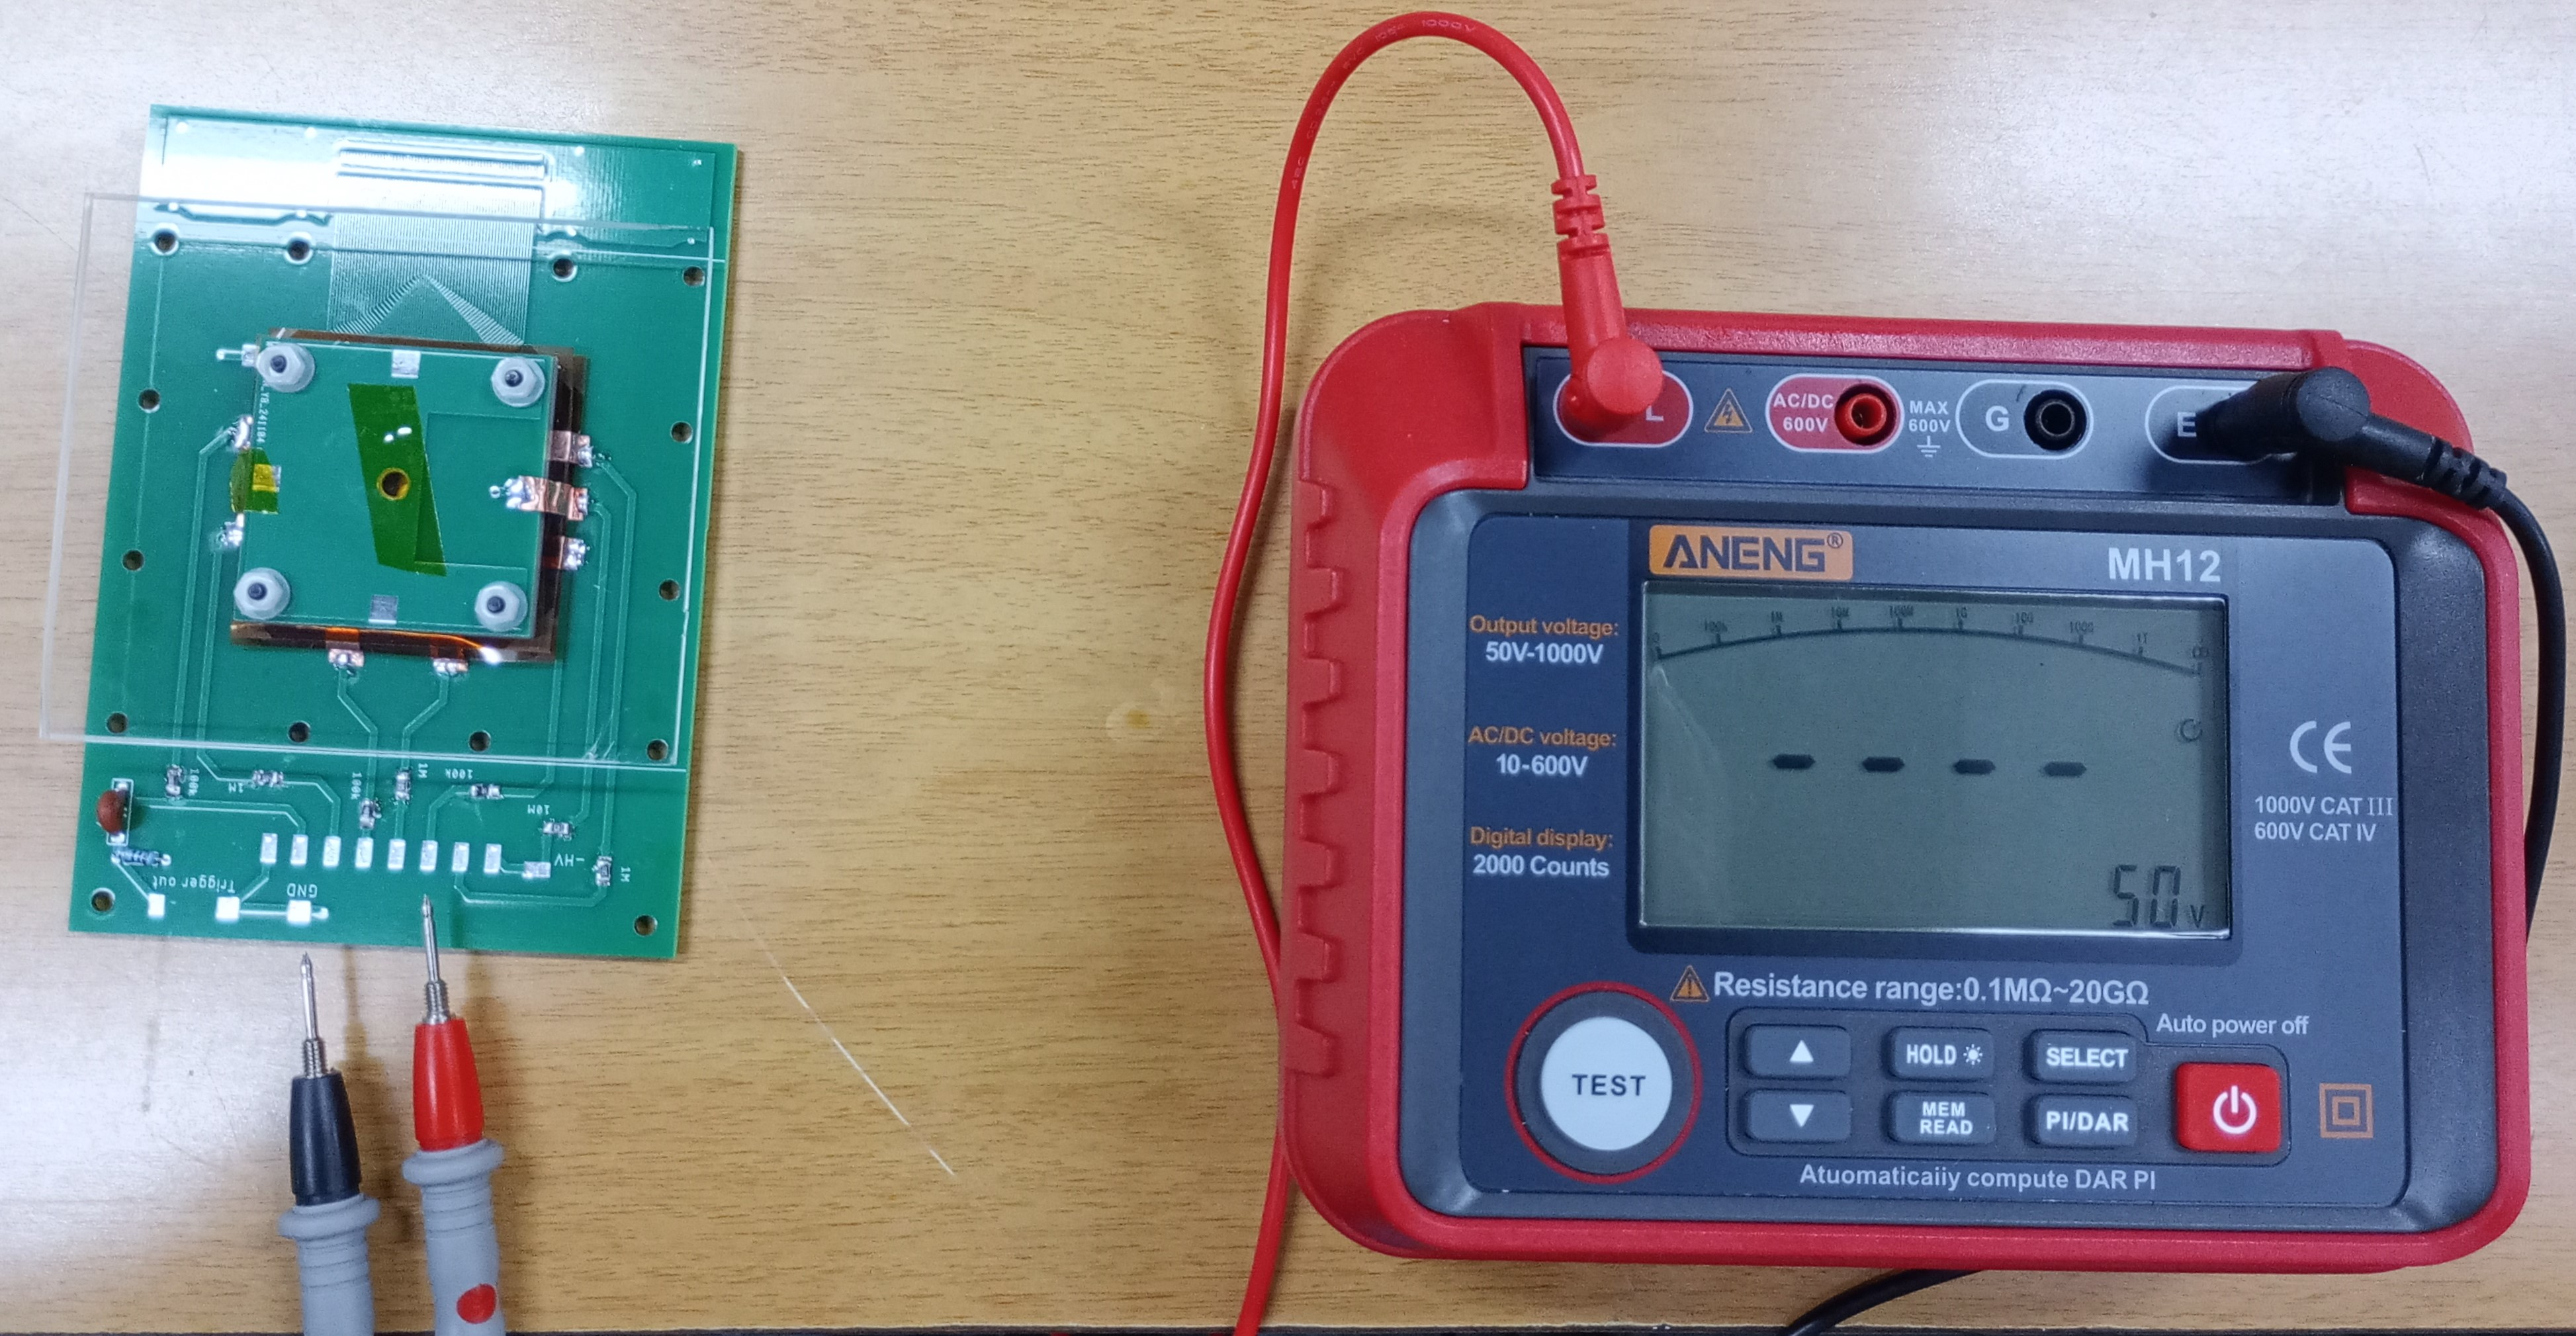
\includegraphics[width=0.7\textwidth]{insulation_test.jpg}
    \caption{Prueba de aislamiento eléctrico en condiciones de alto voltaje.}
    \label{fig:ins_test}
\end{figure}

\noindent Adicionalmente, se diseña y construye un divisor de tensión variable para generar los voltajes necesarios en cada GEM, garantizando así la generación de avalanchas de electrones. Considerando que la fuente de alto voltaje utilizada tiene una capacidad de 5.5 kV y un límite de corriente de 300$\mu A$, se calculan, a partir de la ley de Ohm, los valores de las resistencias que componen el divisor de tensión. En la tabla \ref{fig:divider_table} se presentan los valores obtenidos.  \\

\begin{figure}[H]
    \centering
    \includegraphics[width=0.5\textwidth]{tabla_divider.png}
    \caption{\noindent Tabla de valores de resistencia correspondientes a cada capa de la configuración triple-GEM. A partir de valores de voltaje previamente conocidos, se calculan los valores de las resistencias del divisor de tensión para cada capa utilizando la ley de Ohm. Para la denominación de cada GEM, se adopta la convención GXZ, donde $X$ toma valores entre 1 y 3 para identificar cada una de las tres etapas del triple-GEM, mientras que $Z$ puede ser T (\textit{top}) o B (\textit{bottom}) para indicar la posición dentro de cada GEM.}
    \label{fig:divider_table}
\end{figure}

\noindent El divisor de tensión se implementa en una placa de pruebas utilizando arreglos en serie de potenciómetros de precisión tipo \textit{trimmer} y resistencias de precisión, asegurando una separación adecuada entre los componentes debido a su uso en alto voltaje. De este modo, se logran los valores de resistencia requeridos para cada etapa con una precisión de 0.1 Mohms. A continuación, se lleva a cabo una prueba de medición de la resistencia total del circuito en condiciones de alto voltaje (hasta 1000 V), obteniendo que dicho valor se mantiene constante. Esto indica la ausencia de cortocircuitos en el sistema.  \\

\begin{figure}[H]
    \centering
    \includegraphics[width=0.7\textwidth]{divider_1.jpeg}
    \caption{Implementación y puesta a prueba del divisor de tensión variable. En la fotografía se evidencia la medición de la resistencia total del divisor tensión de $R = 11.39 Mohm$ con aplicación de una diferencia de potencial de aproximadamente 1000V. Comparando con el valor de R total de la tabla \ref{fig:divider_table}, se observa que el valor total de resistencia se mantiene constante en el margen de error de la medición.}
    \label{fig:div1}
\end{figure}

\noindent A continuación, se instala el divisor de tensión y se procede a la soldadura del conector de alto voltaje, así como a la instalación de un filtro RC en el puerto denominado \textit{TRIGGER OUT}, el cual permite probar la señal de detección en el GEM más próximo al \textit{readout} (GEM3 bottom). Asimismo, se suelda el conector Panasonic, encargado de la adquisición de las señales provenientes del plano de \textit{readout}. Además, se coloca el marco plástico, el cual cuenta con orificios de entrada y salida diseñados para el acople rápido de una manguera de poliuretano de 4 mm. Dicho marco incorpora empaques tipo O-ring en ambas caras, lo que garantiza la hermeticidad de la cámara de gas. Por último, se instala la ventana de acrílico de 2 mm de espesor, asegurándola mediante tornillos pasantes metálicos.\\

\begin{figure}[H]
    \centering
    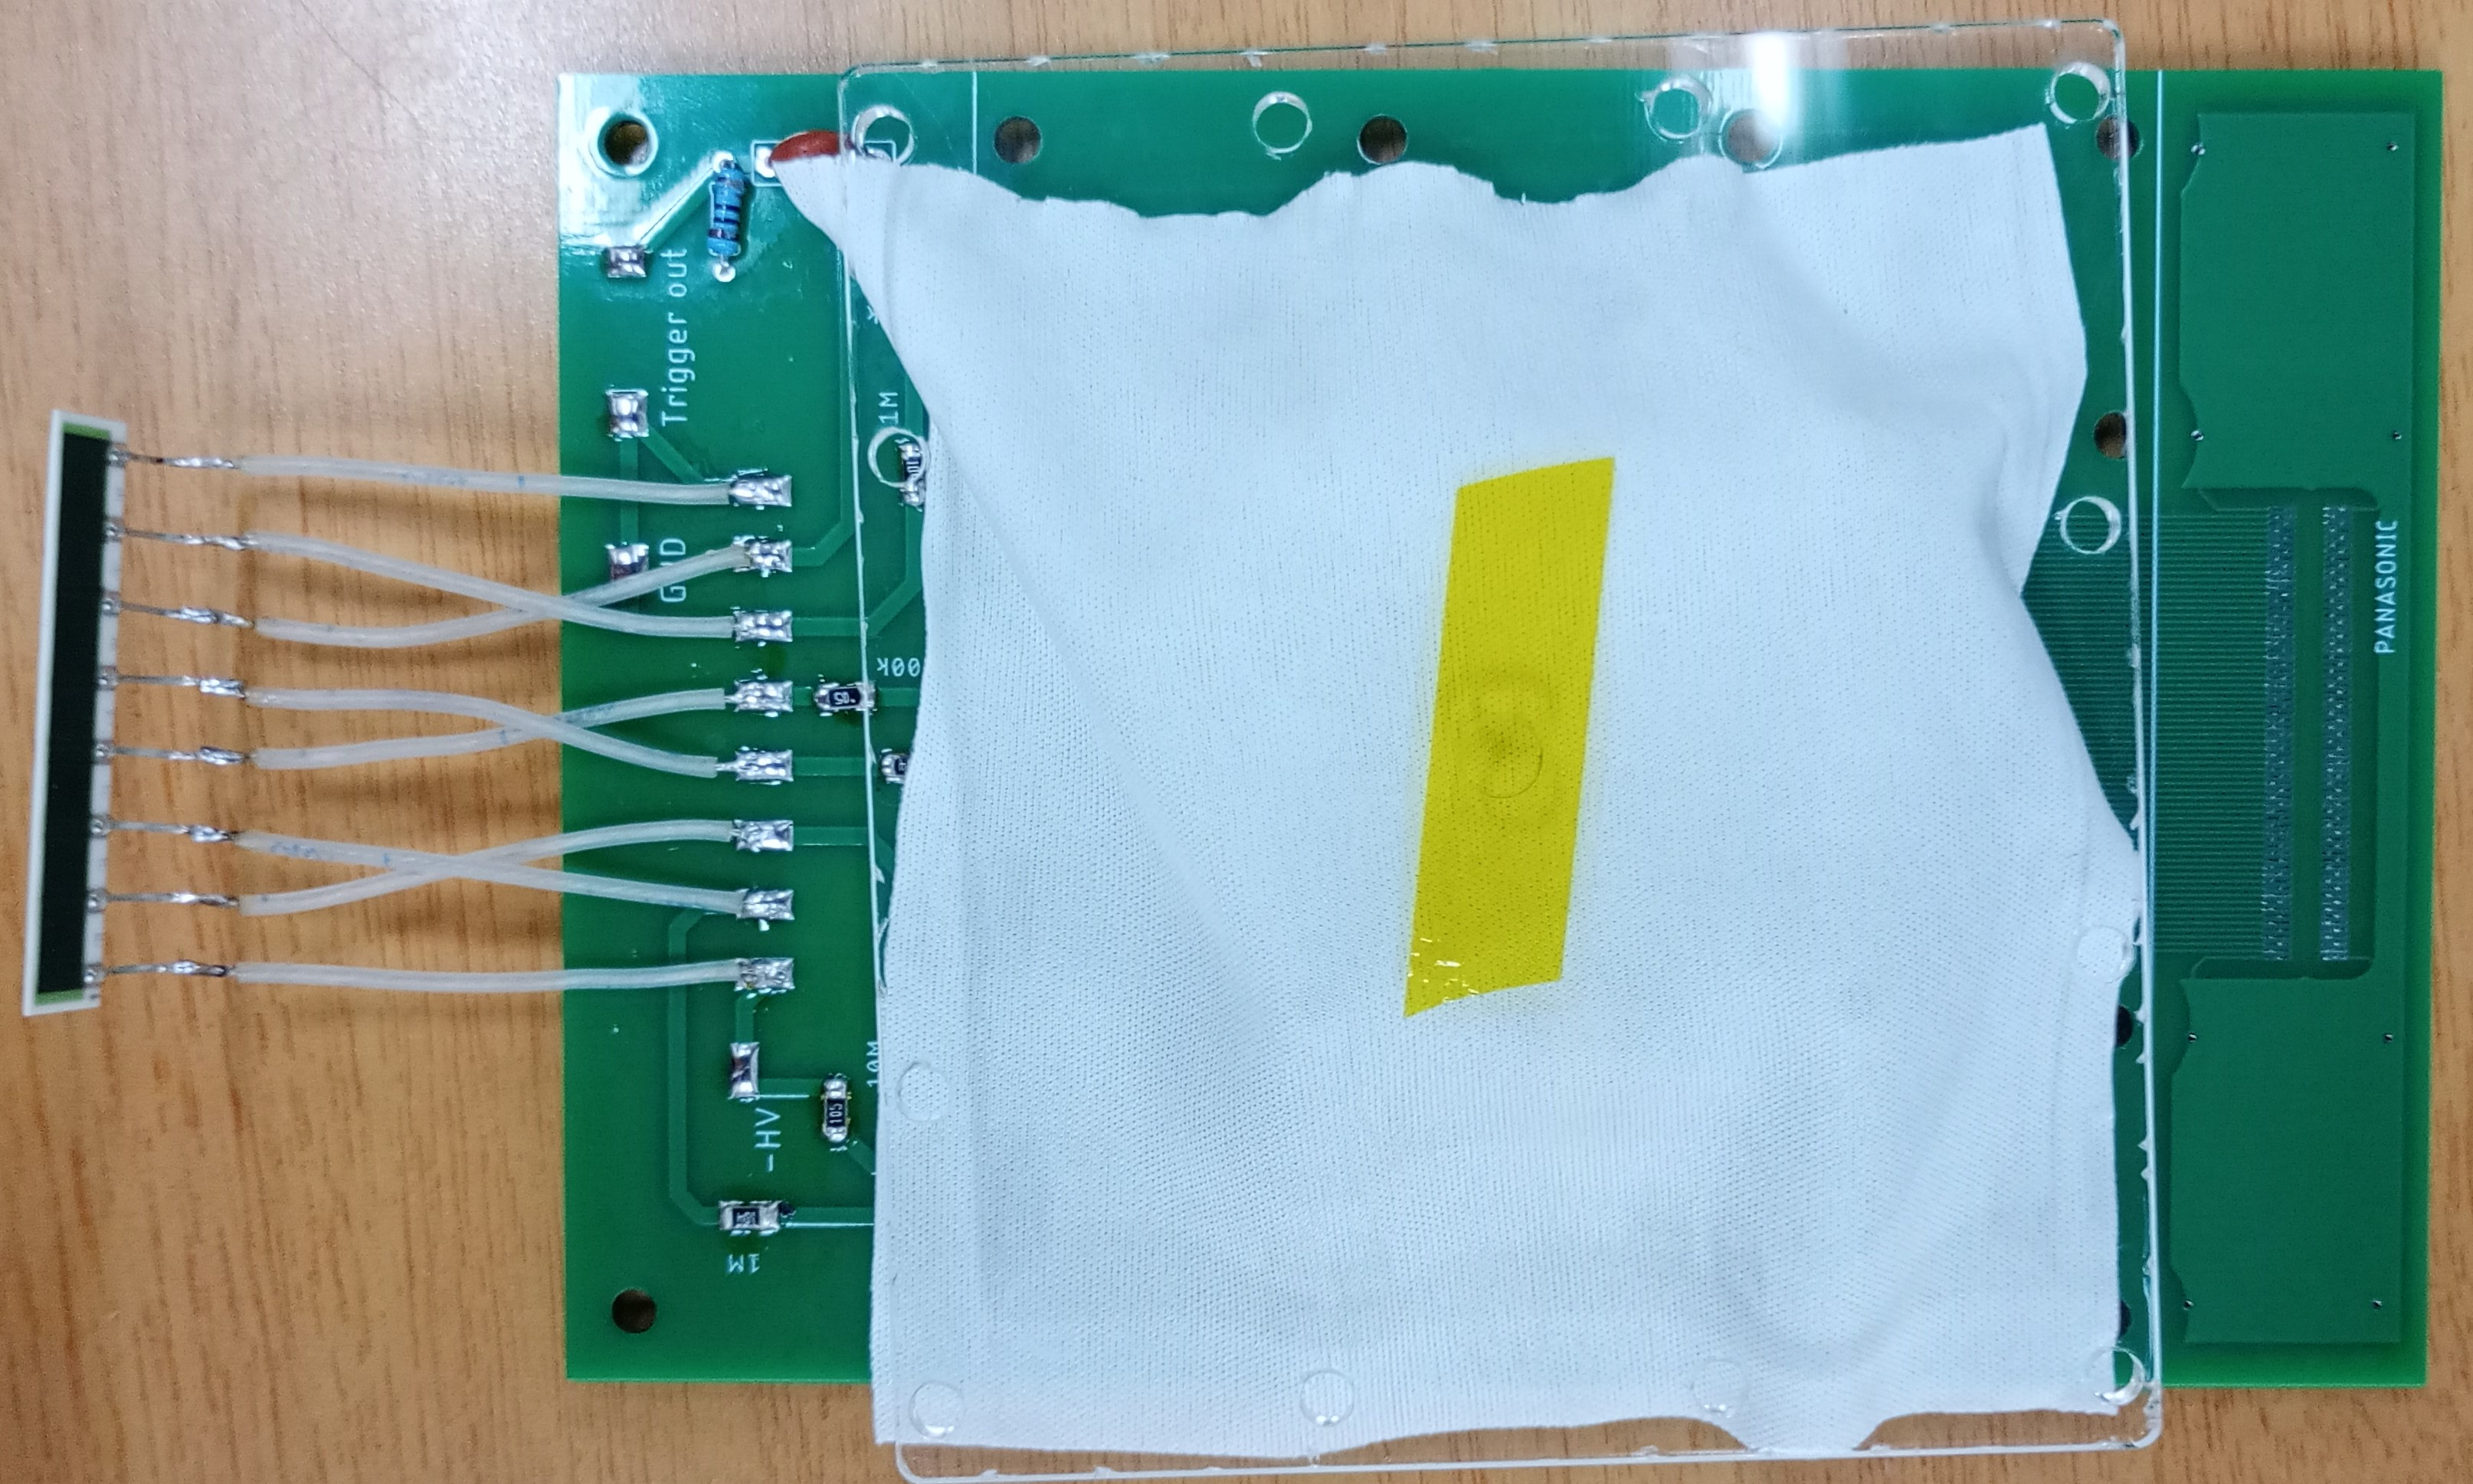
\includegraphics[width=0.7\textwidth]{divider.jpeg}
    \caption{Instalación del divisor de tensión, conector de alto voltaje, filtro RC de \textit{TRIGGER OUT} y cuerpo de la cámara de gas.}
    \label{fig:divider}
\end{figure}

\noindent 

\noindent Para validar el detector, es necesario implementar una cadena de instrumentación especializada que permita su correcto funcionamiento y lectura (véase fig. \ref{fig:setup}). En este caso, se emplean tanto módulos en formato NIM (Nuclear Instrumentation Module) como instrumentos de escritorio. El alto voltaje es suministrado por una fuente programable CAEN 14071, mientras que el gas proviene de un circuito de regulación que se muestra a continuación. La electrónica de lectura del detector está compuesta por un preamplificador y un amplificador lineal ASA LA200A. Adicionalmente, se utiliza un osciloscopio para pruebas de funcionamiento.\\

\noindent El sistema de suministro de gases está compuesto por cilindros de gas puro (Argón y CO2), unidades de regulación de alta a media presión, unidades de media a baja presión, medidores de flujo tipo rotámetro y un mezclador de gases. La proporción de la mezcla que ingresa al mezclador, y posteriormente al detector, se ajusta mediante la lectura de los rotámetros y el control de presión en las unidades de media a baja presión.\\

\begin{figure}[H]
    \centering
    \includegraphics[width=0.7\textwidth]{gas_station.jpeg}
    \caption{Fotografía del sistema de suministro de gases. De derecha a izquierda, se observan el clindro y las unidades de regulación de alta a media presión y las unidades de regulación de media a baja presión.}
    \label{fig:gas_station}
\end{figure}

\begin{figure}[H]
    \centering
    \includegraphics[width=0.6\textwidth]{mixer.jpeg}
    \caption{Fotografía del mezclador de gases.}
    \label{fig:mixer}
\end{figure}
\newpage

\noindent A continuación, se presenta el montaje experimental utilizado para la puesta en funcionamiento y caracterización del detector. En la imagen \ref{fig:setup}, se aprecian las conexiones al sistema de gases, la alimentación de alto voltaje y la salida de señal del detector, la cual pasa por el preamplificador y el amplificador antes de llegar al osciloscopio.\\

\begin{figure}[H]
    \centering
    \includegraphics[width=1\textwidth]{setup_final1.png}
    \caption{Montaje experimental utilizado para el funcionamiento del detector. Se observan los principales componentes: (1) detector ensamblado basado en triple GEM, (2) divisor de tensión variable, (3) preamplificador, (4) crate formato NIM, (5) salida de alto voltaje, (6) osciloscopio, (7) medidores de flujo tipo rotámetros.}
    \label{fig:setup}
\end{figure}

\noindent En la Figura \ref{fig:crate_final} se muestra el resto del montaje experimental utilizado para el funcionamiento del detector. En la imagen se identifican los principales componentes del sistema: el amplificador lineal ASA LA200A, la fuente de alto voltaje programable, que suministra la diferencia de potencial necesaria para la operación del detector; y el osciloscopio, utilizado para la visualización y análisis de la señal adquirida. El sistema se encuentra montado en un \textit{crate} con formato NIM (\textit{Nuclear Instrumentation Module}), un estándar modular ampliamente utilizado en instrumentación nuclear y de partículas. Este formato define dimensiones mecánicas, conexiones eléctricas y especificaciones de alimentación para garantizar la compatibilidad e integración de múltiples módulos electrónicos dentro de una misma unidad.  \\

\begin{figure}[H]
    \centering
    \includegraphics[width=0.9\textwidth]{crate_final.png}
    \caption{Montaje experimental utilizado para el funcionamiento del detector. Se observan los siguientes componentes: (1) amplificador lineal ASA LA200A, (2) fuente de alto voltaje programable CAEN 14071, (3) osciloscopio.}
    \label{fig:crate_final}
\end{figure}

\noindent Para evaluar la capacidad de detección del dispositivo, se coloca una fuente radiactiva de Americio-241 sobre el detector. Para ello, se retira la cinta Kapton que cubre el orificio en el acrílico y se reemplaza por una lámina de vinipel, que permite el paso de las partículas alfa emitidas por la fuente. Además, se emplea un adaptador de conector Panasonic a LEMO, que combina la salida de todos los canales de lectura mediante una compuerta OR, dirigiéndolos a un único canal de salida. Finalmente, la señal resultante se transmite a la cadena de adquisición de datos, permitiendo su visualización en el osciloscopio.

\begin{figure}[H]
    \centering
    \includegraphics[width=0.5\textwidth]{fuentealfa.jpeg}
    \caption{Fotografía del detector ensamblado con la fuente de partículas alfa de Americio-241.}
    \label{fig:fuentealfa}
\end{figure}

\noindent En la Figura \ref{fig:setupalfa} se muestra el montaje experimental en operación, utilizado para caracterizar y verificar el desempeño del detector construido.

\begin{figure}[H]
    \centering
    \includegraphics[width=1\textwidth]{setup_alfa.jpeg}
    \caption{Fotografía del montaje experimental utilizado para validar el funcionamiento del detector.}
    \label{fig:setupalfa}
\end{figure}



%---------------------------------------------------------------------------------------------------------------
\noindent Paralelamente al diseño y construcción del detector con \textit{readout} unidimensional expuesto, se utilizaron los conocimientos adquiridos para proponer un diseño de \textit{readout} bidimensional. Este permitiría, en una futura versión del detector, obtener resolución espacial en dos dimensiones, facilitando la generación de imágenes tipo radiografía, ya sea mediante fuentes continuas como los rayos X o con partículas provenientes de cascadas atmosféricas, dependiendo de la electrónica de lectura utilizada.\\  

\noindent Con el objetivo de desarrollar un plano de lectura bidimensional de bajo costo, se diseñó una matriz de electrodos (véase figura \ref{fig:readout_design}) basada en la técnica \textit{via-in-pad} en una PCB. Los electrodos fueron interconectados estratégicamente en cuatro capas, logrando 32 canales por dimensión, para un total de 64 canales de lectura. Estos canales se agrupan en un conector Hirose, al cual se conectará la electrónica de lectura y el sistema de adquisición de datos.  

\begin{figure}[H]
    \centering
    \includegraphics[width=0.4\textwidth]{readout_design.png}
    \caption{Diseño propuesto para un plano de lectura 2D. Los electrodos circulares corresponden a \textit{vias-in-pad} y las pistas de recolección de señal se diferencian por colores, siendo las azules para la dirección $x$ y las rojas para la dirección $y$. Con el fin de garantizar que no se solapen las señales de dimensiones opuestas, se distribuyen los \textit{vias} en cuatro capas del PCB.  
    }
    \label{fig:readout_design}
\end{figure}

\noindent A partir del concepto planteado, se diseña en software especializado para diseño de PCB la tarjeta de \textit{readout} 2D. Las dimensiones de la matriz de electrodos se establecen según las mismas dimensiones de las láminas GEM, 25 × 25 mm$^2$.\\

\noindent Para determinar el tamaño de los electrodos, se consulta con varios fabricantes de PCB sobre la capacidad de manufactura en la técnica \textit{via-in-pad}, encontrando que la distancia mínima entre electrodos puede ser de 0.675 mm. Esto permite alcanzar hasta 37 canales por dimensión. No obstante, para evitar forzar la manufactura al máximo de resolución y considerando que la electrónica de lectura típicamente cuenta con un número de canales en potencias de 2, se diseña finalmente un plano de lectura de 32 × 32 canales.

\begin{figure}[H]
    \centering
    \includegraphics[width=0.4\textwidth]{readout2D.jpeg}
    \caption{Fotografía del PCB del plano de readout bidimensional propuesto.}
    \label{fig:readout_design_PCB}
\end{figure}

\noindent Asimismo, se diseña un PCB para el plano de \textit{drift} que se acople al factor de forma del plano de lectura. Las perspectivas de este trabajo apuntan a utilizar la experiencia y el conocimiento obtenidos en el diseño e implementación del sistema de detección 1D para desarrollar un detector eficaz capaz de generar imágenes tipo radiografía.  

\begin{figure}[H]
    \centering
    \includegraphics[width=0.4\textwidth]{drift2D.jpeg}
    \caption{Fotografía del PCB del plano de drift para un detector bidimensional propuesto.}
    \label{fig:drift_design}
\end{figure}

\newpage
\section{Resultados}

\noindent Teniendo en cuenta que el objetivo principal de este capítulo es la construcción de un detector basado en la configuración triple-GEM, los resultados obtenidos incluyen tanto la caracterización del detector como la validación de su funcionamiento básico. Una de las características críticas de su operación es garantizar los voltajes adecuados para cada capa GEM de la pila, lo cual se logra mediante el divisor de tensión. Por lo tanto, uno de los resultados más relevantes es comprobar la linealidad del divisor de tensión construido hasta el régimen de alto voltaje, ya que su estabilidad es fundamental para asegurar la eficacia en la generación de avalanchas de electrones.\\ 

\noindent En la figura \ref{fig:result_divisor} se presenta un gráfico de corriente versus voltaje obtenido a partir de datos experimentales extraídos de la interfaz de monitoreo de la fuente de alto voltaje programable. Se realizó un barrido manual de voltaje en incrementos de aproximadamente 100 V, esperando alrededor de 10 segundos en cada paso para permitir la estabilización de los valores antes de registrar la corriente consumida por el detector. El barrido se extendió hasta los 3000 V utilizando exclusivamente gas argón. A partir de este punto, se observaron descargas y la fuente activó el mecanismo de apagado de emergencia o \textit{trip}. La incertidumbre asociada al voltaje, según el sistema de monitoreo de la fuente de alto voltaje, es de 0.1 V, mientras que la incertidumbre en la corriente es de 0.01 $\mu$A. No obstante, las barras de error en el gráfico son indistinguibles debido a la escala y el rango del barrido.\\   

\noindent A partir de la tabla \ref{fig:divider_table} y las mediciones realizadas durante la implementación del divisor de tensión variable, se observa que la resistencia total del divisor es de $11.3 \pm 0.1$ Mohm. No obstante, este valor se obtuvo en condiciones de bajo voltaje. Por lo tanto, para verificar la estabilidad de este valor y, en consecuencia, la estabilidad de las diferencias de potencial eléctrico en los distintos gaps asociados a cada GEM de la pila, se aplica una regresión lineal a los datos experimentales. Esto permite obtener el parámetro de pendiente de la recta, que, por comparación directa con la ecuación de la ley de Ohm $V = RI$, corresponde a la resistencia total del divisor de tensión. El resultado obtenido es de $1.13 \times 10^{7}$ ohm, lo que confirma que la resistencia total del divisor se mantiene estable en el rango de voltaje de funcionamiento del detector.


\begin{figure}[H]
    \centering
    \includegraphics[width=1\textwidth]{result_divisor.png}
    \caption{Curva de I vs V caracteristica del divisor de tensión con gas argón. Se busca comprobar la linealidad del comportamiento del divisor en el régimen de alto voltaje.}
    \label{fig:result_divisor}
\end{figure}

\begin{figure}[H]
    \centering
    \includegraphics[width=1\textwidth]{pulso1.png}
    \caption{pulso}
    \label{fig:pulso2}
\end{figure}

\begin{figure}[H]
    \centering
    \includegraphics[width=1\textwidth]{pulso2.png}
    \caption{pulso}
    \label{fig:pulso1}
\end{figure}

\newpage
\section{Análisis de resultados}

%-------------------------------------------------------------------------------------------------------------------
\newpage
\chapter{\centering Sistemas de Adquisición de Datos}

\vspace{1cm}


% \noindent La instrumentación científica es uno de los pilares fundamentales en la investigación, ya que permite a los científicos observar y medir fenómenos físicos con una precisión que trasciende los límites de los sentidos humanos. Desde la exploración del universo hasta el estudio de procesos microscópicos, la tecnología ha evolucionado para capturar señales, transformarlas y convertirlas en información significativa. En este contexto, el proceso de medición va más allá de la simple observación; implica una interacción activa entre el objeto de estudio y los sistemas diseñados para adquirir datos, conocidos como sistemas de adquisición de datos (DAQ). Estos sistemas no solo registran la información, sino que también la procesan para hacerla accesible y comprensible.\\

% \noindent En efecto, los sistemas de adquisición de datos desempeñan un papel crucial en la investigación científica y en diversas áreas de la ingeniería. Estos dispositivos capturan señales provenientes de sensores que, mediante procesos de conversión, transforman fenómenos físicos como la temperatura, presión, radiación o aceleración, en señales eléctricas. Dichas señales eléctricas, a su vez, son procesadas y convertidas en datos digitales, listos para ser analizados y visualizados. Así, debido a la amplia gama de magnitudes físicas que pueden medirse, resulta imprescindible el uso de sensores especializados que garanticen una conversión precisa y efectiva de estas magnitudes en señales eléctricas manejables por el sistema de adquisición.\\

% \noindent Otro factor crucial en los sistemas de adquisición de datos modernos es su capacidad para procesar información en tiempo real. Esto ha sido posible gracias al uso de tecnologías digitales como los procesadores de señal digital (DSP), las matrices de puertas programables (FPGA) y los circuitos integrados de aplicación específica (ASIC). Estas herramientas permiten que los sistemas DAQ realicen cálculos complejos y análisis de datos en fracciones de segundo, lo cual es especialmente útil en aplicaciones que requieren respuestas rápidas, como la monitorización médica o los experimentos de alta energía en física.\\

% \noindent Una característica importante de los sistemas de adquisición de datos es la capacidad de almacenar y transferir grandes volúmenes de información. En muchos casos, los datos deben ser almacenados para su análisis posterior, o bien ser transmitidos de manera rápida y eficiente a otros sistemas. Los métodos de transmisión pueden variar dependiendo de la aplicación, e incluyen desde tecnologías convencionales como USB y Ethernet, hasta buses especializados como GPIB o PCIe en entornos industriales y de investigación de alta complejidad.\\

% \noindent Por último, la presentación de los datos al usuario es un componente esencial en cualquier sistema DAQ. Las interfaces gráficas de usuario (GUI) permiten visualizar de manera intuitiva los datos obtenidos, facilitando la interpretación de los resultados por parte del investigador. Esta capacidad de presentar datos en tiempo real permite ajustar las mediciones de acuerdo con las necesidades del experimento, brindando un control dinámico sobre el proceso de adquisición.\\

% \noindent En este capítulo, se describirán los conceptos fundamentales de los sistemas de adquisición de datos, abordando sus principales componentes y tecnologías. Asimismo, se analizarán ejemplos prácticos en diversas disciplinas científicas y técnicas, proporcionando una visión general de cómo estas herramientas son esenciales en la investigación moderna. También se explorarán los desafíos y soluciones para implementar un sistema DAQ eficiente, destacando su importancia en el desarrollo de proyectos experimentales.\\

\noindent La instrumentación científica ha sido un pilar fundamental en el avance de la ciencia y la tecnología, al permitir a los investigadores observar y analizar fenómenos que trascienden los límites de la percepción humana. Desde la exploración del cosmos hasta la manipulación de partículas subatómicas, la capacidad de medir, registrar y procesar datos con precisión ha ampliado de manera significativa los horizontes del conocimiento en múltiples disciplinas. Los avances en tecnología de medición han facilitado la captura de señales complejas, que al ser transformadas en datos utilizables, proporcionan información crítica para la comprensión de fenómenos naturales y artificiales. En este contexto, los sistemas de adquisición de datos (DAQ, por sus siglas en inglés) desempeñan un rol esencial, actuando como el enlace entre los fenómenos físicos observados y su representación digital. Estos sistemas permiten registrar una vasta gama de magnitudes físicas—como temperatura, presión, aceleración o radiación—a partir de sensores que las convierten en señales eléctricas, que pueden ser procesadas y analizadas con precisión. La eficiencia con la que estos sistemas capturan y procesan dichas señales es crucial, especialmente en situaciones donde los eventos ocurren a escalas temporales extremadamente breves o cuando la precisión es determinante para la interpretación fiable de los datos obtenidos \cite{sinclair1}.\\

\noindent Los sistemas DAQ no solo son indispensables en la investigación científica básica, sino que también tienen aplicaciones vitales en sectores industriales, médicos y tecnológicos avanzados. En campos como la astrofísica, la física de partículas o la ingeniería de materiales, la capacidad de registrar con exactitud eventos transitorios o señales de baja intensidad es crucial para obtener información precisa sobre los procesos subyacentes. Por ejemplo, en experimentos de colisionadores de partículas, los sistemas DAQ permiten monitorear interacciones subatómicas en tiempo real, donde las señales generadas por los detectores ocurren en escalas temporales minúsculas y requieren ser capturadas con alta resolución tanto temporal como espacial. Asimismo, en la detección de radiación, ya sea en contextos de protección radiológica o de investigación nuclear, los DAQ juegan un papel fundamental al registrar las interacciones ionizantes y convertirlas en datos procesables. Esto permite analizar fuentes de radiación o eventos de baja probabilidad, que de otro modo pasarían desapercibidos en el ruido de fondo. La importancia de los DAQ radica en su capacidad para gestionar grandes volúmenes de datos, procesando señales con rapidez y precisión para obtener información que de otra forma sería inaccesible o ininterpretada \cite{gutleber2008data}.\\

\noindent Dentro de las tecnologías empleadas para el desarrollo de estos sistemas, los dispositivos basados en Field Programmable Gate Arrays (FPGA) han adquirido una posición destacada. Su capacidad para procesar datos a gran velocidad y en tiempo real, con una latencia mínima, los convierte en una opción ideal para aplicaciones que requieren un tratamiento eficiente de señales complejas. Además, los FPGA ofrecen una flexibilidad notable en su configuración, permitiendo la implementación de arquitecturas optimizadas para tareas específicas, como el procesamiento de señales de alta velocidad o la reducción de ruido en entornos de alta sensibilidad \cite{meyer2007digital}. Esta versatilidad es especialmente relevante en la detección de partículas y radiación, donde la precisión y la velocidad de procesamiento son elementos cruciales para asegurar que las interacciones físicas sean correctamente registradas y analizadas.\\

\noindent En este trabajo, se presenta el desarrollo de un marco teórico que explica los conceptos fundamentales involucrados en la cadena de manejo de información en un sistema de adquisición de datos (DAQ). Se aborda desde las interacciones de los sistemas físicos con los sensores, hasta las etapas electrónicas involucradas en el tratamiento y digitalización de las señales. Además, se profundiza en las plataformas comúnmente utilizadas para el procesamiento de datos, incluyendo las tecnologías más avanzadas, como los sistemas basados en FPGA, y su posterior comunicación con el usuario a través de diversas interfaces. Este capítulo también incluye una sección dedicada al montaje experimental, en la cual se describen detalladamente los componentes y la configuración implementada, así como las herramientas de hardware y software empleadas para desarrollar un DAQ optimizado para aplicaciones de alto rendimiento, como la adquisición de datos de detectores de radiación. Finalmente, se presenta una sección de resultados, en la que se valida el funcionamiento del sistema mediante la adquisición de señales sintéticas. A través de esta fase experimental, se ponen a prueba las distintas etapas y configuraciones del DAQ, seguido de un análisis de los datos obtenidos. Este análisis no solo busca verificar el desempeño del sistema, sino que también se plantean conclusiones y perspectivas para el desarrollo futuro en este campo.

\newpage

\section{Marco teórico}
\noindent En esta sección, se abordarán los fundamentos necesarios para comprender el funcionamiento y la implementación de sistemas de adquisición de datos, basándose en una descripción detallada de los principales componentes y procesos involucrados. La explicación comenzará con una visión general de los sistemas físicos e interacciones, proporcionando el contexto necesario para entender cómo los fenómenos físicos son detectados e interpretados a través de sistemas instrumentales. A continuación, se discutirá el papel crucial de los sensores y detectores en la conversión de magnitudes físicas en señales eléctricas, seguido por un análisis de las señales eléctricas de sensores, que detalla cómo se generan y las características que definen estas señales. Posteriormente, se explorará el tratamiento y acondicionamiento de señales, un proceso fundamental para asegurar que las señales obtenidas sean adecuadas para su procesamiento. El procesamiento digital (digital processing) se abordará a continuación, cubriendo las técnicas y plataformas comúnmente utilizadas para convertir las señales acondicionadas en datos útiles y analizables. La discusión también incluirá la interfaz de comunicación (communication interface), que es clave para la transferencia eficiente de datos entre el sistema de adquisición y otros dispositivos, así como su impacto en la eficiencia general del sistema. Finalmente, se revisará la interfaz de usuario (user interface), destacando la importancia de una representación clara y accesible de los datos para facilitar el análisis y la toma de decisiones. Para facilitar la comprensión de estos conceptos, se presenta la figura \ref{fig:DAQ_generic}, que ilustra el diagrama de los principales componentes de un sistema de adquisición de datos genérico. Esta figura proporciona una visión integral de la cadena de etapas, desde la adquisición de señales físicas hasta su presentación final al usuario, y servirá como referencia visual a lo largo de la discusión.

\begin{figure}[h]
    \centering
    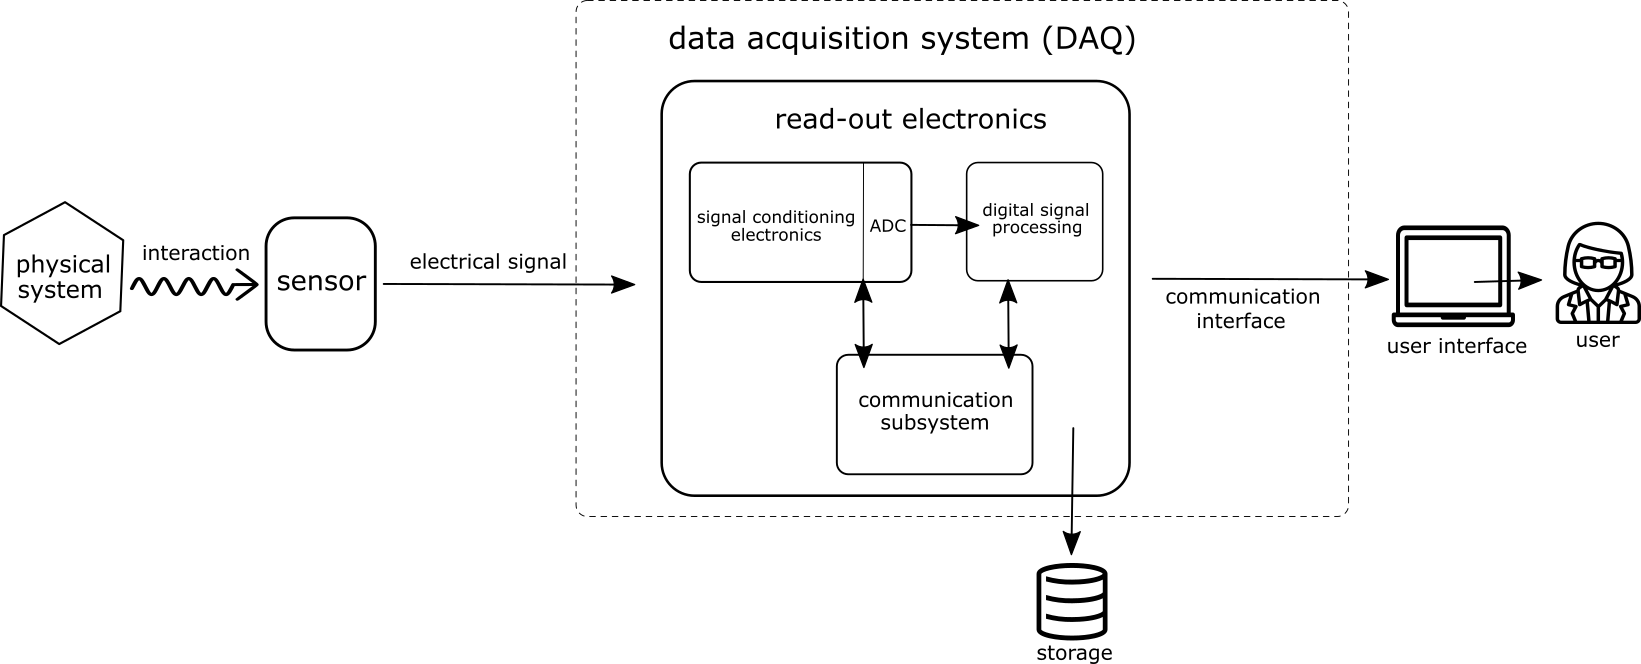
\includegraphics[width=1.0\textwidth]{DAQ_chain.png}
    \caption{Diagrama de los principales componentes de un sistema de adquisición de datos para la medición de un sistema físico. El flujo de información comienza con un sistema físico que interactúa con un sensor o detector, generando una señal eléctrica. Esta señal es adquirida y procesada por la electrónica de lectura, la cual incluye subetapas como el acondicionamiento de la señal y el procesamiento digital. Posteriormente, los datos procesados son transferidos a través de una interfaz de comunicaciones hacia el usuario, quien accede a ellos mediante una interfaz de usuario, permitiendo su visualización y análisis.}
    \label{fig:DAQ_generic}

\end{figure}
\subsection{Sistemas físicos e interacciones}

\noindent En el campo de la instrumentación científica, un sistema físico se refiere a cualquier entidad u objeto cuyas propiedades y comportamientos son susceptibles de estudio mediante técnicas de medición y observación. Estos sistemas pueden abarcar desde las partículas subatómicas, que siguen las leyes de la mecánica cuántica, hasta sistemas macroscópicos como materiales sólidos, fluidos, y sistemas biológicos, además de fenómenos astrofísicos de gran escala.\\

\noindent Un sistema físico se caracteriza por poseer ciertas propiedades mensurables, como la temperatura, la presión, el campo eléctrico o magnético, y la energía, entre otras. Dichas propiedades pueden ser modificadas o perturbadas por interacciones externas, lo que permite que sean explotadas para generar señales que puedan ser medidas. Es en este contexto donde los sistemas físicos se vuelven de interés para la adquisición de datos: a través de la manipulación o el monitoreo de las interacciones que estos sistemas tienen con su entorno, es posible extraer información relevante que caracterice su comportamiento \cite{o1785essay}.\\

\noindent Para lograr esta interacción, es necesario comprender de manera exhaustiva la naturaleza del sistema físico y cómo sus propiedades responden ante estímulos específicos. Esta comprensión es clave para el diseño de sensores y detectores que, mediante la transformación de las propiedades físicas en señales eléctricas, permiten la extracción sistemática de información. Es fundamental que el sistema físico interactúe de manera controlada con el sensor para que la información obtenida sea representativa de las magnitudes físicas de interés y no de variables externas o perturbaciones no deseadas.\\

\noindent En particular, un ejemplo notable lo constituyen las partículas fundamentales y el transporte de energía a partir de estas, conocido como radiación \cite{knoll1}. Dependiendo de sus propiedades físicas —como la carga, masa o energía—, es posible diseñar experimentos que permitan su interacción controlada con medios materiales, lo que facilita su estudio. Por ejemplo, las partículas cargadas, como los electrones, protones o muones, pueden provocar ionización en el medio por el que atraviesan, liberando pares de electrones e iones. Esta recolección de carga, medida a través de señales eléctricas, permite extraer información sobre la energía, trayectoria o tipo de partícula. Detectores de ionización, como cámaras de gas o semiconductores, explotan este principio para realizar análisis precisos de las propiedades físicas de las partículas.\\

\noindent Además de la ionización, otras propiedades como el momento o la energía de las partículas pueden inferirse a partir de las señales que generan durante su interacción con el sistema de detección. Esto permite no solo estudiar fenómenos como transiciones de estado y decaimientos radiactivos, sino también obtener datos que contribuyen al entendimiento de la composición y dinámica de las partículas en diversas condiciones experimentales. Así, la interacción entre sistemas físicos y los detectores es clave para extraer información que impulse el conocimiento en áreas como la física de partículas y la astrofísica.

\subsection{Sensores y detectores}

\noindent Como se expuso anteriormente, un sensor es un dispositivo que responde a un estímulo físico, químico o biológico específico, y genera una señal de tipo eléctrico, que tiene una relación funcional con la magnitud del estímulo. Los sensores suelen estar compuestos por dos componentes principales: el elemento sensible o transductor, que interactúa directamente con el estímulo (por ejemplo, temperatura, presión, luz) y un mecanismo de conversión que traduce la respuesta del transductor en una señal utilizable (como una corriente o voltaje eléctrico). La precisión, sensibilidad, resolución y rango de operación son características clave que determinan el rendimiento de un sensor \cite{webster1}.\\

\noindent Los sensores se pueden clasificar según diversos criterios \cite{sinclair3}: por el tipo de magnitud que miden, el principio de funcionamiento (resistivos, capacitivos, inductivos, piezoeléctricos), el tipo de señal de salida (analógicos, digitales), la forma de operación (activos, pasivos), y la naturaleza del contacto con la magnitud medida (de contacto, sin contacto). Además, según su contexto de uso, los sensores pueden ser clasificados como domésticos (utilizados en electrodomésticos y dispositivos de consumo), industriales (empleados en automatización y control de procesos), o científicos (destinados a investigación y aplicaciones especializadas).\\

\noindent En particular, estos últimos destacan por su alta precisión, exactitud, sensibilidad, robustez y fiabilidad. Su objetivo es proporcionar mediciones extremadamente precisas y reproducibles, ya que los resultados son cruciales para investigaciones avanzadas. Además, suelen poseer un amplio rango dinámico, lo que les permite detectar tanto variaciones muy pequeñas como extremadamente grandes en las magnitudes de interés. Un ejemplo destacado en este grupo son los detectores de radiación o partículas, que sobresalen por su capacidad para interactuar con corpúsculos a nivel atómico y subatómico, generando señales pulsadas que revelan propiedades esenciales de las partículas incidentes, como su energía, momento lineal o trayectoria, entre otras \cite{knoll2}.\\

\noindent Existen diferentes tipos de detectores de partículas, cada uno optimizado para aplicaciones específicas. Los detectores de estado sólido, como los semiconductores de silicio, son ampliamente utilizados por su alta resolución espacial y temporal. Estos dispositivos funcionan mediante la creación de pares electrón-hueco cuando una partícula cargada atraviesa el material, generando una señal eléctrica proporcional a la energía depositada. Por otro lado, los detectores gaseosos, como las cámaras de ionización o los contadores proporcionales, operan en medios gaseosos donde la ionización del gas produce electrones libres y iones positivos que se colectan para formar una señal. Estos detectores son valiosos por su capacidad para cubrir grandes volúmenes, lo que es esencial en experimentos que requieren la detección de partículas en áreas extensas. Además, existen otros tipos de detectores como los cintiladores, que emiten luz cuando son excitados por radiación ionizante, y los detectores Cherenkov, que detectan partículas cargadas moviéndose a velocidades superiores a la velocidad de la luz en un medio dado \cite{kolanoski1}.

\subsection{Señales eléctricas de sensores}

\noindent Dado que las señales eléctricas son esenciales en este contexto como portadoras de la información física que se busca extraer, es fundamental describir sus principales características para comprender cómo las etapas electrónicas del sistema de adquisición de datos (DAQ) las afectan. Aunque las señales pueden ser digitales o análogas, generalmente las producidas por un sensor o detector son de tipo análogo. \\

\noindent Una señal analógica proveniente de un sensor se caracteriza principalmente por su variación continua en el tiempo y su capacidad para representar información en un rango infinito de valores. La amplitud de la señal refleja la magnitud del parámetro medido, como temperatura o presión, y puede variar suavemente en respuesta a cambios en el entorno. La frecuencia de la señal puede no ser relevante en todos los casos, pero el tiempo de respuesta y la estabilidad son cruciales para asegurar mediciones precisas. Además, la señal puede estar afectada por ruido y errores, lo que requiere técnicas de filtrado y calibración para obtener datos confiables. La forma de onda de la señal es continua y puede ser analizada en el dominio del tiempo para evaluar su comportamiento y en el dominio de la frecuencia para identificar componentes relevantes \cite{sinclair2}. En la figura \ref{fig:generic_signal}, se ilustra una señal en el dominio del tiempo proveniente de un sensor de aceleración.\\

\begin{figure}[H]
    \centering
    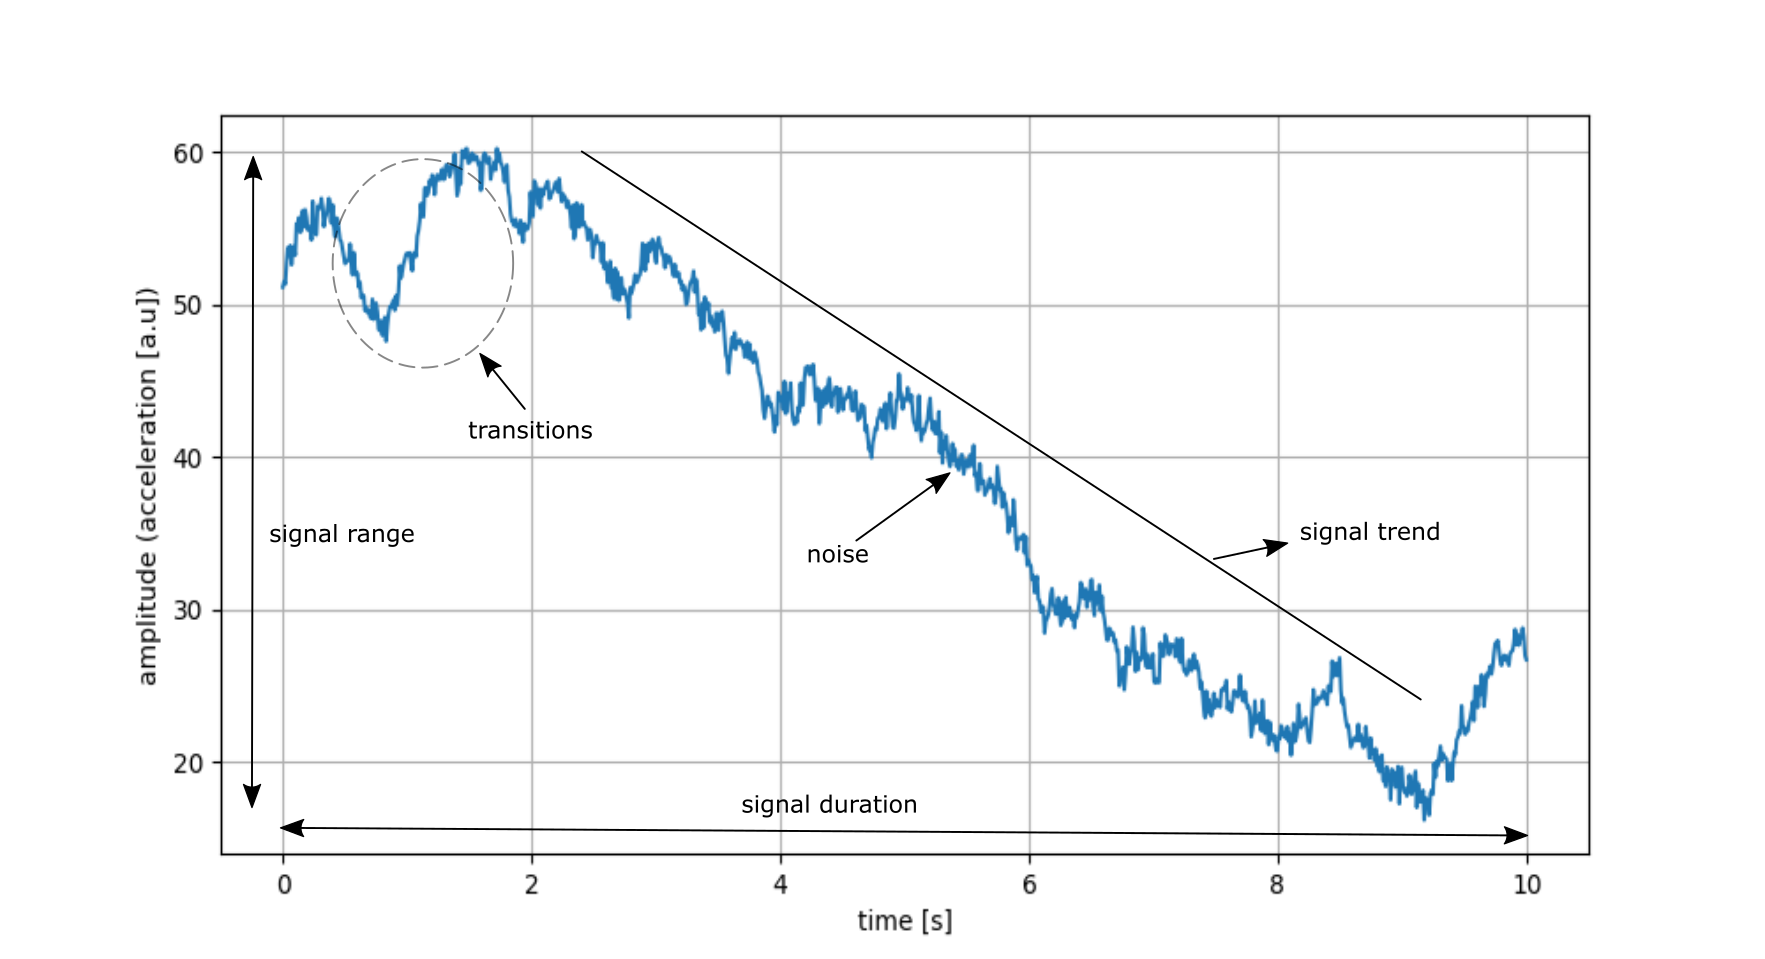
\includegraphics[width=1.0\textwidth]{mysignal.png}
    \caption{Señal no periódica en el dominio del tiempo proveniente de un sensor de aceleración. En ella es posible observar algunas características como duración, rango de la magnitud de interés en el lapso registrado, ruido electrónico, tendencia y transitorios. La amplitud de la señal solo puede ser definida con base a un nivel de referencia.}
    \label{fig:generic_signal}

\end{figure}

\noindent Un caso de particular interés son las señales producidas por los detectores de partículas, que en general son de naturaleza pulsada \cite{kolanoski1}. En este contexto, se puede asociar la detección de un evento con una perturbación localizada, denominada pulso, que se define sobre la línea base de la señal de salida. La figura \ref{fig:pulse} muestra un ejemplo genérico de un pulso individual, utilizado para ilustrar algunas de sus características principales.

\begin{figure}[H]
    \centering
    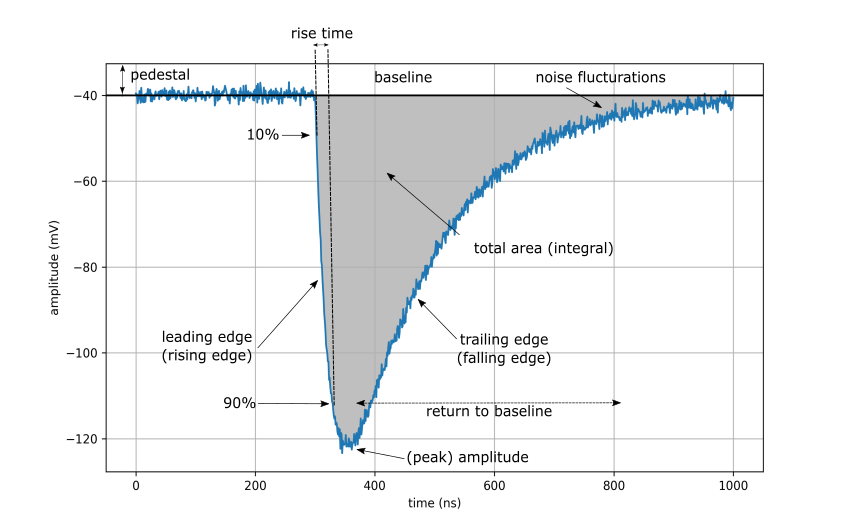
\includegraphics[width=1.0\textwidth]{pulse_edited.png}
    \caption{Diagrama ilustrativo de las principales características de un pulso típico de un detector de radiación. Reproducido a partir de \cite{kolanoski2}}
    \label{fig:pulse}

\end{figure}

\noindent Según \cite{kolanoski2}, suponiendo que la señal generada por el detector es corta comparado con los tiempos típicos de procesamiento de la electrónica de lectura, las cantidades que caracterizan un pulso son:

\begin{itemize}
    \item La amplitud máxima del pulso: también conocida como altura del pulso, es el valor máximo que alcanza la señal. En sistemas lineales, este valor es proporcional a la energía primaria depositada en el detector.
    \item Tiempo de pico: Es el momento en el tiempo en el que se alcanza la amplitud máxima del pulso.
    \item Área o integral del pulso: Representa el área bajo la curva del pulso. En sistemas lineales y para señales cortas tipo $\delta$, su valor debería ser proporcional a la energía primaria depositada.
    \item Ancho del pulso: Se refiere a la duración del pulso, que generalmente se define como el ancho total a la mitad de la altura máxima (FWHM, por sus siglas en inglés).
    \item Bordes de subida y bajada: Son las pendientes ascendente y descendente del pulso.
    \item Tiempo de subida: Caracteriza la rapidez con la que el pulso aumenta. Comúnmente se define como el tiempo necesario para que el pulso pase del 10\% al 90\% de su amplitud máxima, aunque existen otras definiciones.
    \item Tasa de variación (Slew rate): Indica el cambio de voltaje por unidad de tiempo $dV/dt$ y se expresa en unidades de $V/s$.
    \item Línea base o valor de pedestal: Es el valor de salida cuando no hay ninguna señal de entrada. Define el nivel 'cero' desde el cual se mide la altura de la señal. Aunque generalmente la línea base tiene un valor fijo, pueden ocurrir desviaciones durante un cierto (y breve) período de tiempo. Estas desviaciones se conocen como desplazamientos de la línea base.
    \item Tiempo de retorno a la línea base: Es el tiempo necesario para que la amplitud del pulso vuelva al valor de la línea base.
    \item Suboscilación: Se refiere a la parte de la amplitud de un pulso que tiene un signo opuesto (con respecto a la línea base) en comparación con la amplitud principal.
    \item Señal unipolar: Es una forma de pulso en la que, salvo por las fluctuaciones de ruido, el valor de la amplitud se mantiene por encima o por debajo de la línea base en todo momento $t$. Por lo general, también se incluyen en esta definición las señales con pequeñas suboscilaciones.
    \item Señal bipolar: Es una forma de pulso en la que la parte del pulso que ocurre más tarde en el tiempo tiene un signo opuesto al de la parte que ocurre primero.
\end{itemize}

\noindent Por otro lado, las señales digitales, esenciales en el procesamiento de información, se caracterizan por su naturaleza discreta tanto en el tiempo como en la amplitud, en tanto que solo pueden adoptar dos estados, representados por los valores 1 y 0. Es de resaltar, que las señales analógicas tratadas anteriormente, son convertidas a digitales mediante un dispositivo denominado conversor análogo digital o ADC. Adicionalmente. a partir de una señal digital base con frecuencia constante, conocida como reloj, se puede codificar información en señales digitales mediante código binario y operaciones de conteo. Básicamente, se mide cuántos ciclos de reloj la señal permanece en un estado u otro. Esta metodología es altamente versátil, ya que permite realizar operaciones matemáticas utilizando el sistema binario \cite{brown2000fundamentals}. En la figura \ref{fig:digital_siganl} se puede observar un ejemplo de señal digital para ilustrar.

\begin{figure}[H]
    \centering
    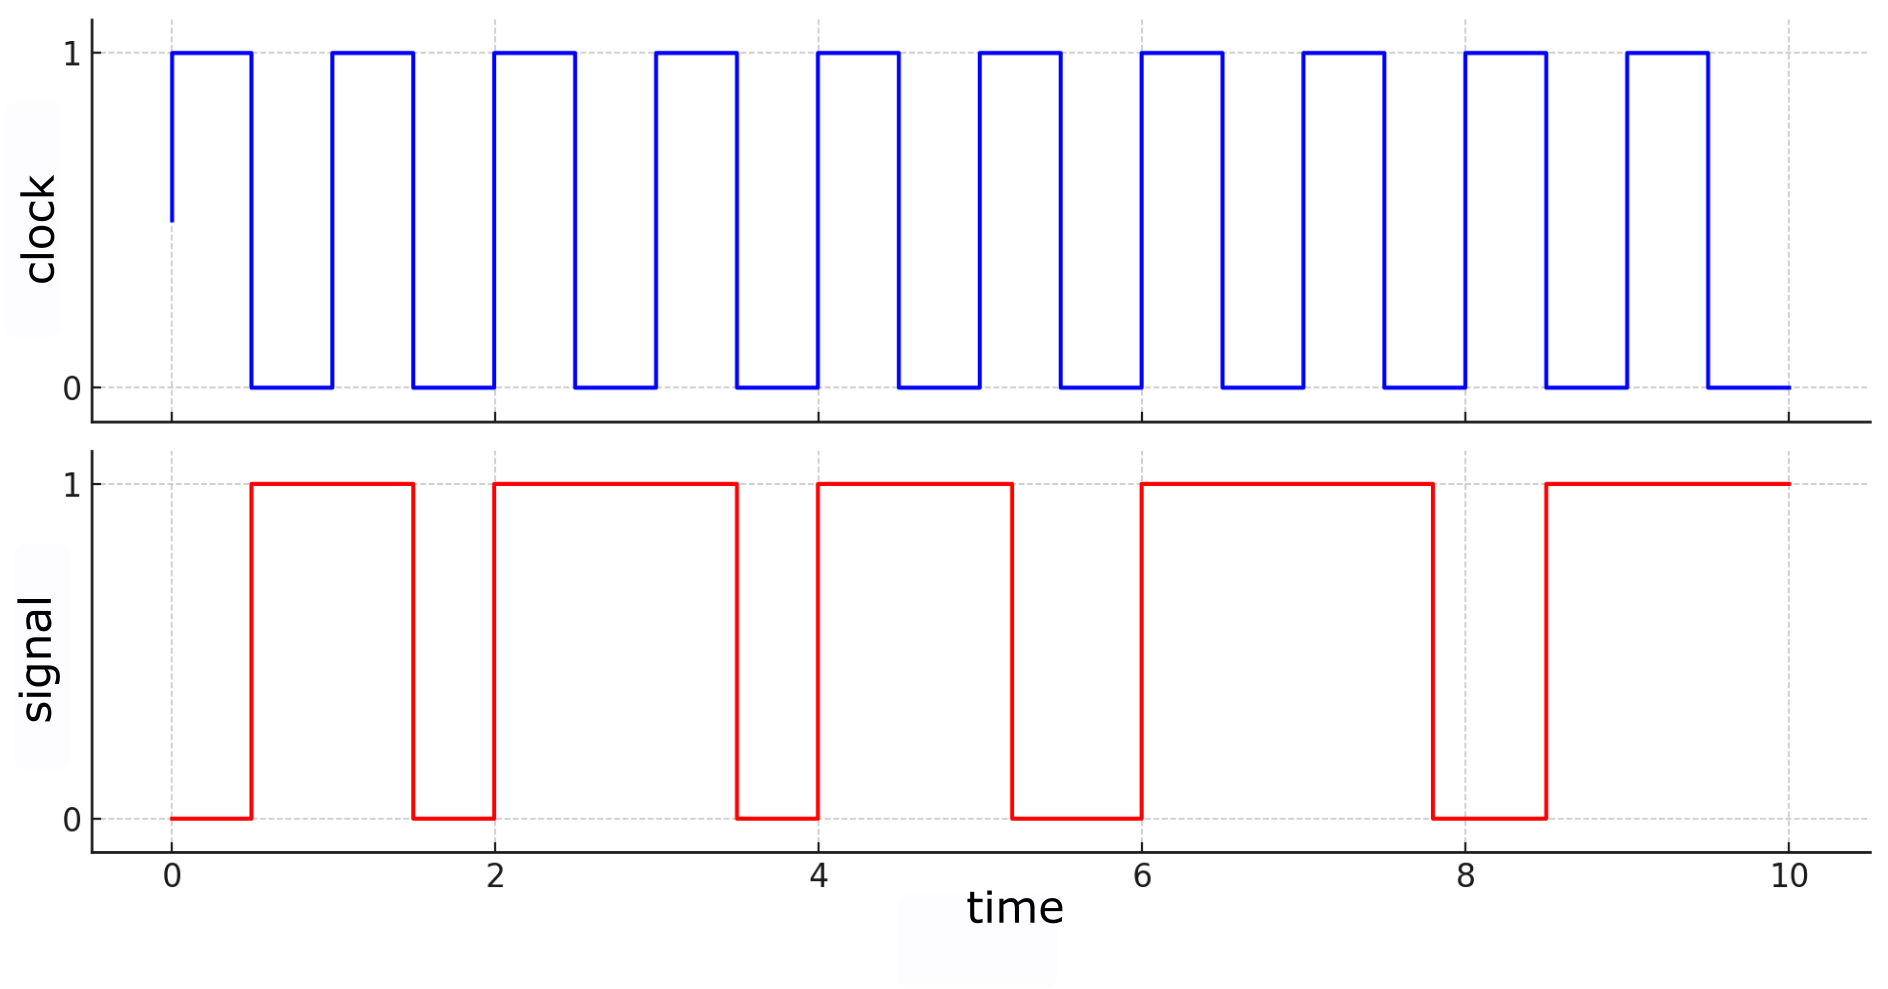
\includegraphics[width=0.7\textwidth]{digital_signal.png}
    \caption{Ejemplo de diagrama de tiempo de una señal digital. En la parte superior se muestra una señal típica de reloj y en la parte inferior una señal genérica con información codificada en su estado (ampitud) o en su duración (ancho).}
    \label{fig:digital_siganl}

\end{figure}

\subsection{Tratamiento y acondicionamiento de señales}

\noindent Próxima al sensor, se encuentra la etapa de tratamiento y acondicionamiento, que típicamente comprende electrónica analógica para la amplificación, shaping y digitalización de la señal. Esta etapa es esencial para filtrar y modular la señal, otorgándole las características adecuadas para ser transferida a las etapas de procesamiento digital posteriores. En la figura \ref{fig:generic_frontend} se observa un esquema genérico de esta sección de la cadena de adquisición de datos.\\

\begin{figure}[h]
    \centering
    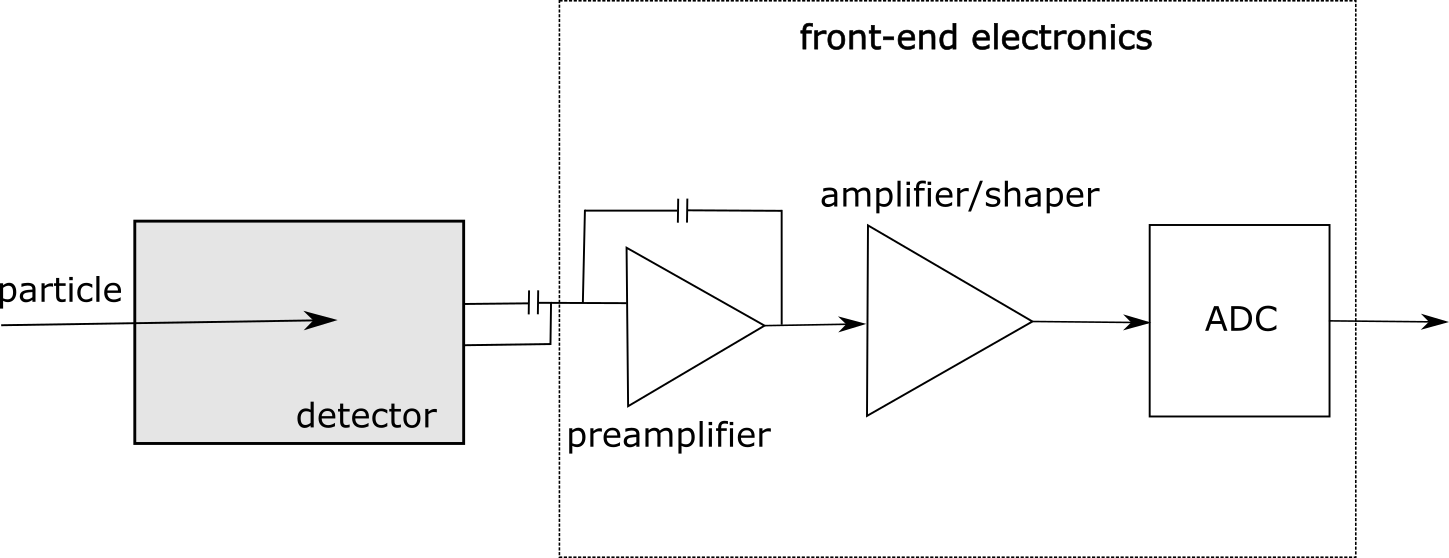
\includegraphics[width=0.8\textwidth]{front-end.png}
    \caption{Un esquema de una etapa de electrónica de acondicionamiento típico, utilizado a menudo para la lectura de un detector, que incluye amplificación, conformación de impulsos y digitalización (representada aquí por un ADC).}
    \label{fig:generic_frontend}

\end{figure}

\noindent Los sistemas involucrados en esta etapa, deben cumplir con tres características: (a) ser causales, (b) invariantes en el tiempo, y (c) lineales al menos en la primera etapa de amplificación. Un sistema se considera causal si, en cualquier momento, solo depende del valor de su entrada en ese instante. Es invariante en el tiempo si la relación entre la salida y la entrada, por ejemplo, el ratio $\text{señal}_{\text{entrada}}/\text{señal}_{\text{salida}}$ no varía con el tiempo \cite{kolanoski3}. La linealidad del sistema implica que la señal de salida (por ejemplo, $v_{out(t)}$) no depende del tamaño de la señal de entrada (por ejemplo, $i_{in(t)}$), esto es, 
\begin{equation}
    v_{\text {out }}\left(\alpha \times i_{\text {in }}(t)\right)=\alpha \times v_{\text {out }}\left(i_{\text {in }}(t)\right)
\end{equation}

\noindent En muchos casos, la magnitud a la salida de un sensor puede ser muy pequeña, por lo que es necesario implementar etapas de preamplificación y amplificación que aumenten la amplitud de la señal (ganancia) hasta que esta se encuentre en el rango de sensibilidad de las etapas posteriores. Para llevar a cabo tal función, es posible utilizar dintintos dispositivos, sin embargo, los más comunes son los amplificadores operacionales y transistores. Usualmente las señales de entrada provenients del sensor o detector al preamplificador son transformadas en señales de voltaje $(V)$ o de corriente $(I)$. Dependiento de los tipos de entrada y salida, es posible distinguir \cite{kolanoski4}:

\begin{itemize}
    \item amplificador de voltaje: $V \rightarrow V$,
    \item amplificador de corriente: $I \rightarrow I$,
    \item amplificador de transconductancia: $V \rightarrow I$,
    \item amplificador de transimpedancia: $I \rightarrow V$,
    \item amplificador de carga: $Q \rightarrow V$ (o $I$).
\end{itemize}

\noindent Como expone \cite{knoll3}, La función principal del preamplificador es captar la señal del detector sin deteriorar notablemente la relación señal-ruido (SNR) inherente. Por ello, el preamplificador se ubica generalmente lo más cerca posible del detector para reducir la carga capacitiva $(C)$ sobre este. Por ejemplo, un preamplificador de voltaje amplifica directamente la señal de voltaje $V_{\text{in}}$, manteniendo una alta impedancia de entrada $Z_{\text{in}}$ y una baja impedancia de salida $Z_{\text{out}}$ para asegurar una transferencia eficiente y reducir la influencia del ruido. En ambos casos, la linealidad del preamplificador es crucial para que la relación $V_{\text{out}}/ V_{\text{in}}$ se mantenga constante, lo cual es esencial para la precisión en la medición \cite{leo1994techniques}.\\

\noindent Por otro lado, un preamplificador de carga convierte una señal de carga $Q$ generada por el detector en un voltaje proporcional $V$, dada la relación: 

\begin{equation}
    V = \frac{Q}{C}
\end{equation}

La figura \ref{fig:preamp} ilustra su comportamiento típico sobre la señal del detector.\\

\begin{figure}[H]
    \centering
    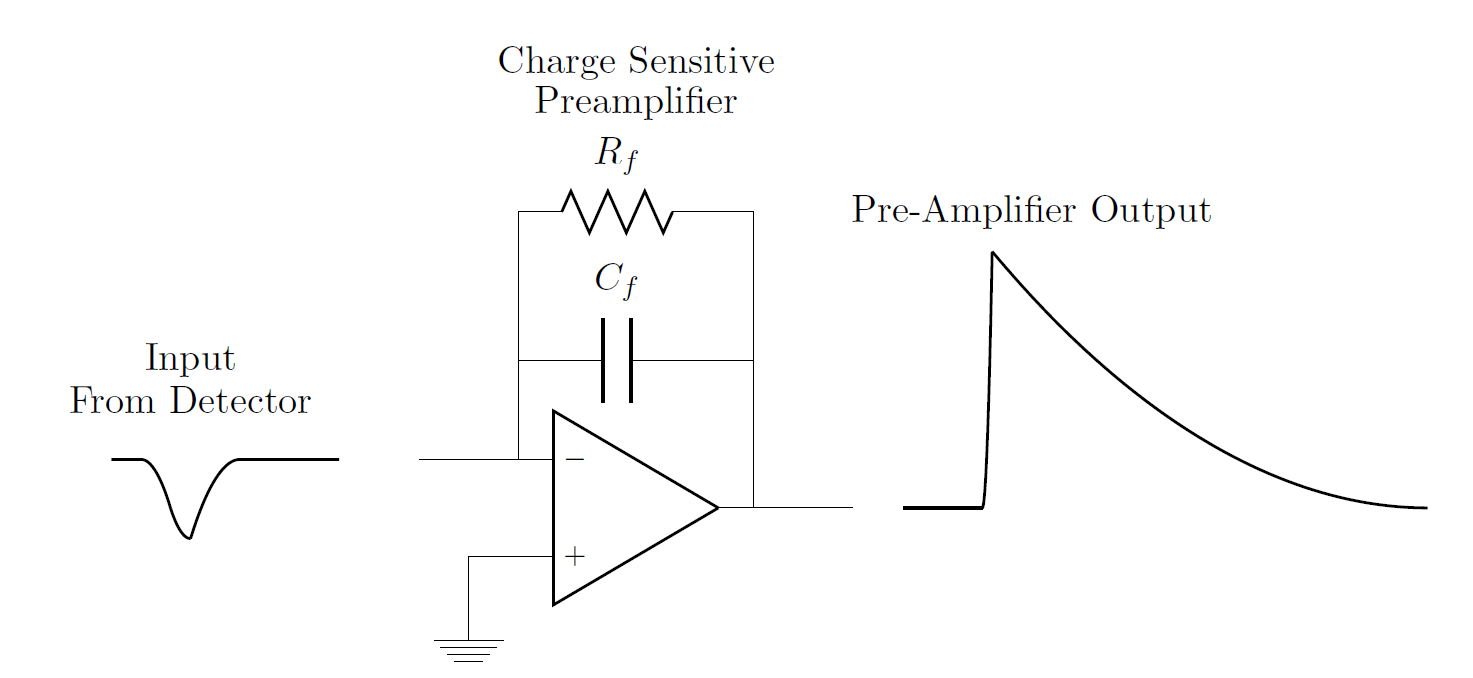
\includegraphics[width=0.8\textwidth]{preamp.PNG}
    \caption{Diagrama que ilustra la estructura y comportamiento típico de un preamplificador de carga. En este se observa la señal de salida de un detector de carga, los componentes electrónicos del preamplificador y la señal típica de salida de este. Tomado de \cite{kolanoski4}.}
    \label{fig:preamp}

\end{figure}

\noindent La amplificación por etapas de una señal ofrece numerosas ventajas significativas. Principalmente, permite reducir el ruido generado en cada etapa individual, resultando en una señal final más limpia y menos propensa a la distorsión. Este método también mejora la estabilidad del sistema al distribuir la amplificación, evitando la saturación que podría ocurrir con una amplificación intensa en una sola etapa. Además, facilita el control preciso de la ganancia y la adaptación de impedancias entre diferentes componentes, lo cual mejora la eficiencia y la transferencia de la señal. Esta amplificación gradual es particularmente útil para manejar señales débiles, amplificándolas sin riesgo de distorsión. Asimismo, distribuye la carga térmica generada, disminuyendo el riesgo de sobrecalentamiento de los componentes \cite{webster1}. \\

\noindent La etapa de amplificación principal generalmente se realiza mediante un amplificador operacional con una resistencia en realimentación. Como modelo matemático, el detector, representado como una capacitancia a descargar, suministra la señal de corriente $i_{s}$ a través de la resistencia $R_{s}$ a un nivel de referencia en un tiempo $\Delta t$. Si el tiempo de descarga es grande comparado al tiempo de duración de la señal 

\begin{equation}
    \left(\tau=R_S C_D \gg\right. \Delta t)
\end{equation}

en cierto sentido, el detector integra la señal de corriente en la capacitancia del detector 

\begin{equation}
    \left(V_D=Q_S / C_D\right) 
\end{equation}

y a la entrada del amplificador se tiene el voltaje 

\begin{equation}
    v_{\text{in}}(t)=V_D \exp \left(-t / R_S C_D\right)
\end{equation}

\noindent El voltaje de salida es proporcional a $v_{i n}$ y el sistema opera como un amplificador de voltaje \cite{kolanoski6}:


\begin{equation}
    v_{\text {out }}(t)=-\frac{R_f}{R_S} v_{\text {in }}(t)=-\frac{R_f V_D}{R_S} \exp \left(-t / R_S C_D\right) .
\end{equation}


\subsubsection{Tratamiento y acondicionamiento de señales: Signal shaping}

\noindent En la cadena de tratamiento de señales, la etapa de \textit{shaping} es un circuito electrónico fundamental que modifica la forma de una señal para optimizar su calidad y adaptarla a los requisitos del procesamiento subsiguiente. Esta etapa generalmente se integra en la fase de preamplificación o amplificación y es especialmente relevante en sistemas de detección de partículas. Su función principal es transformar señales pulsadas, que pueden presentar formas diversas, en pulsos uniformes y bien definidos. Esta uniformidad es crucial para evitar la superposición de pulsos (\textit{pile-up}) (fig. \ref{fig:pile_up}) y disminuir el ruido mediante un filtrado eficiente de frecuencia \cite{leo1994techniques}.

\begin{figure}[H]
    \centering
    \includegraphics[width=0.6\textwidth]{pile_up.PNG}
    \caption{Ejemplos de eventos de pile-up en un detector. El gráfico muestra dos casos de superposición de señales donde dos pulsos ocurren en rápida sucesión, lo que provoca la combinación de sus amplitudes. El ejemplo 1 (línea roja) y el ejemplo 2 (línea azul punteada) ilustran cómo la proximidad temporal de los pulsos afecta la forma y altura de las señales medidas, causando distorsión en la resolución temporal y energética. Tomado de \cite{luo2018pulse}}
    \label{fig:pile_up}
\end{figure}

\noindent Los pulsos electrónicos generados por el preamplificador tienen tiempos de decaimiento típicos que varían entre unos pocos nanosegundos y varios microsegundos. Si llegan señales adicionales durante el tiempo de decaimiento, puede ocurrir pile-up a pesar de que el capacitor de retroalimentación del preamplificador se descargue. Para mitigar esto, se utilizan filtros pasa-altos y pasa-bajos, que permiten separar las señales superpuestas y moldear los pulsos de salida en formas más Gaussianas. Además, los filtros ayudan a reducir el ruido blanco que afecta a todas las frecuencias, mejorando así la SNR \cite{kolanoski5}. La figura \ref{fig:shaper} ilustra las formas de pulsos típicos en la salida del preamplificador que ingresan una configuración de shaping básica compuesta por un circuito CR-RC. Usualmente se observa una caída (undershoot) en la salida del shaper, la cual se corrige con la cancelación polo-cero.\footnote{Técnica de diseño de circuitos que anula efectos indeseados al colocar un cero en la misma frecuencia que un polo, mejorando la respuesta del sistema.} \\

\begin{figure}[h]
    \centering
    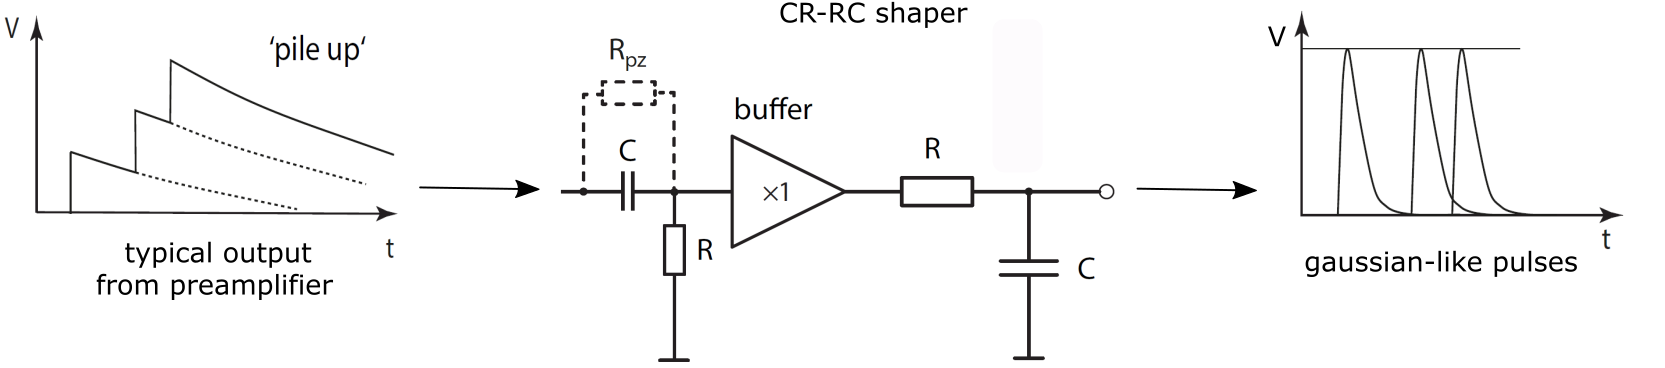
\includegraphics[width=1.0\textwidth]{shaper_chain.png}
    \caption{Funcionamiento típico de un shaper. La resistencia $R_{\text{pz}}$ paralela al condensador del filtro de paso alto se utiliza para la corrección del undershooting. El amplificador (×1) entre las secciones del filtro de paso de banda sirve como un buffer, impidiendo que el filtro de paso bajo aplique una carga significativa al filtro de paso alto. Adaptado de \cite{kolanoski5}.}
    \label{fig:shaper}
\end{figure}

\noindent Es importante señalar que el proceso de shaping puede realizarse en la etapa de procesamiento digital, adaptándose a las necesidades específicas de la aplicación. Formas de pulso, como la trapezoidal, que resultan complejas de generar mediante electrónica analógica, pueden implementarse de manera más eficiente en el dominio digital utilizando filtros con parámetros ajustables en plataformas configurables como las FPGA \cite{radeka1968optimum}. Este enfoque se explorará en mayor detalle en la sección \ref{sec:digital_processing}. Asimismo, dependiendo de los requisitos del usuario, otros subsistemas, como los discriminadores de señales y los circuitos de trigger, pueden implementarse tanto mediante comparadores analógicos como a través de algoritmos de comparación en la etapa de procesamiento digital.

\subsubsection{Tratamiento y acondicionamiento de señales: Digitalización}
\noindent De acuerdo con \cite{meyer2007digital}, la digitalización de las señales provenientes de sensores es crucial debido a la precisión y flexibilidad que ofrece frente a los métodos analógicos tradicionales. Con el avance de los convertidores analógico-digitales (ADC) de alta velocidad y buena resolución desde los años 90, la posibilidad de procesar digitalmente las señales de los sensores se ha consolidado.\\

\noindent Las ventajas de este enfoque incluyen una flexibilidad ilimitada en la elección de parámetros de procesamiento, mayor estabilidad al eliminar el riesgo de derivas debido a cambios de temperatura o voltaje, y la capacidad de realizar análisis más detallados con múltiples salidas de un mismo sensor. Además, la manipulación digital no introduce ruido adicional y permite la implementación precisa de formas de señal que serían difíciles o imposibles de lograr en circuitos analógicos. Sin embargo, una desventaja potencial es la limitación en la precisión temporal, ya que los sistemas digitales están restringidos a la frecuencia de muestreo más cercana, lo que puede ser menos exacto que los métodos analógicos en aplicaciones que requieren una temporización muy rápida.\\

\noindent La función principal de un ADC (Convertidor Analógico-Digital) es transformar una señal de tensión analógica en un código digital proporcional, manteniendo esta conversión de manera continua a una frecuencia determinada por el reloj del sistema. Una ilustración genérica de su principio de funcionamiento se observa en la figura \ref{fig:adc_basic}. 

\begin{figure}[h]
    \centering
    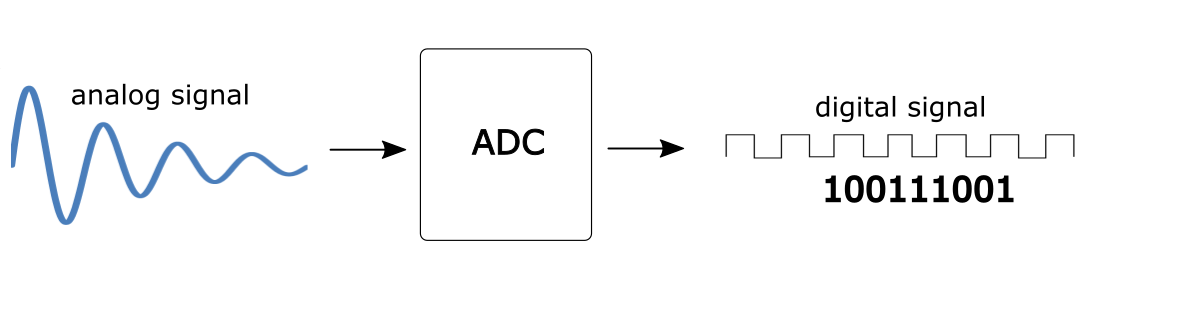
\includegraphics[width=0.8\textwidth]{adc_basic.png}
    \caption{Representación del principio de funcionamiento de un ADC. Una señal eléctrica analógica ingresa al convertidor analógico-digital ADC y genera una señal digital, que codifica mediante representación binaria la información de la señal original.}
    \label{fig:adc_basic}
\end{figure}

\noindent Por ejemplo, un reloj operando a 500 MHz permite una velocidad de muestreo de 500 MSPS (Megamuestras por segundo), lo que corresponde a una muestra cada 2 ns. En la figura \ref{fig:adc_out} se muestra la simulación de una señal senoidal proveniente de un sensor, digitalizada mediante un ADC con estas características.

\begin{figure}[h]
    \centering
    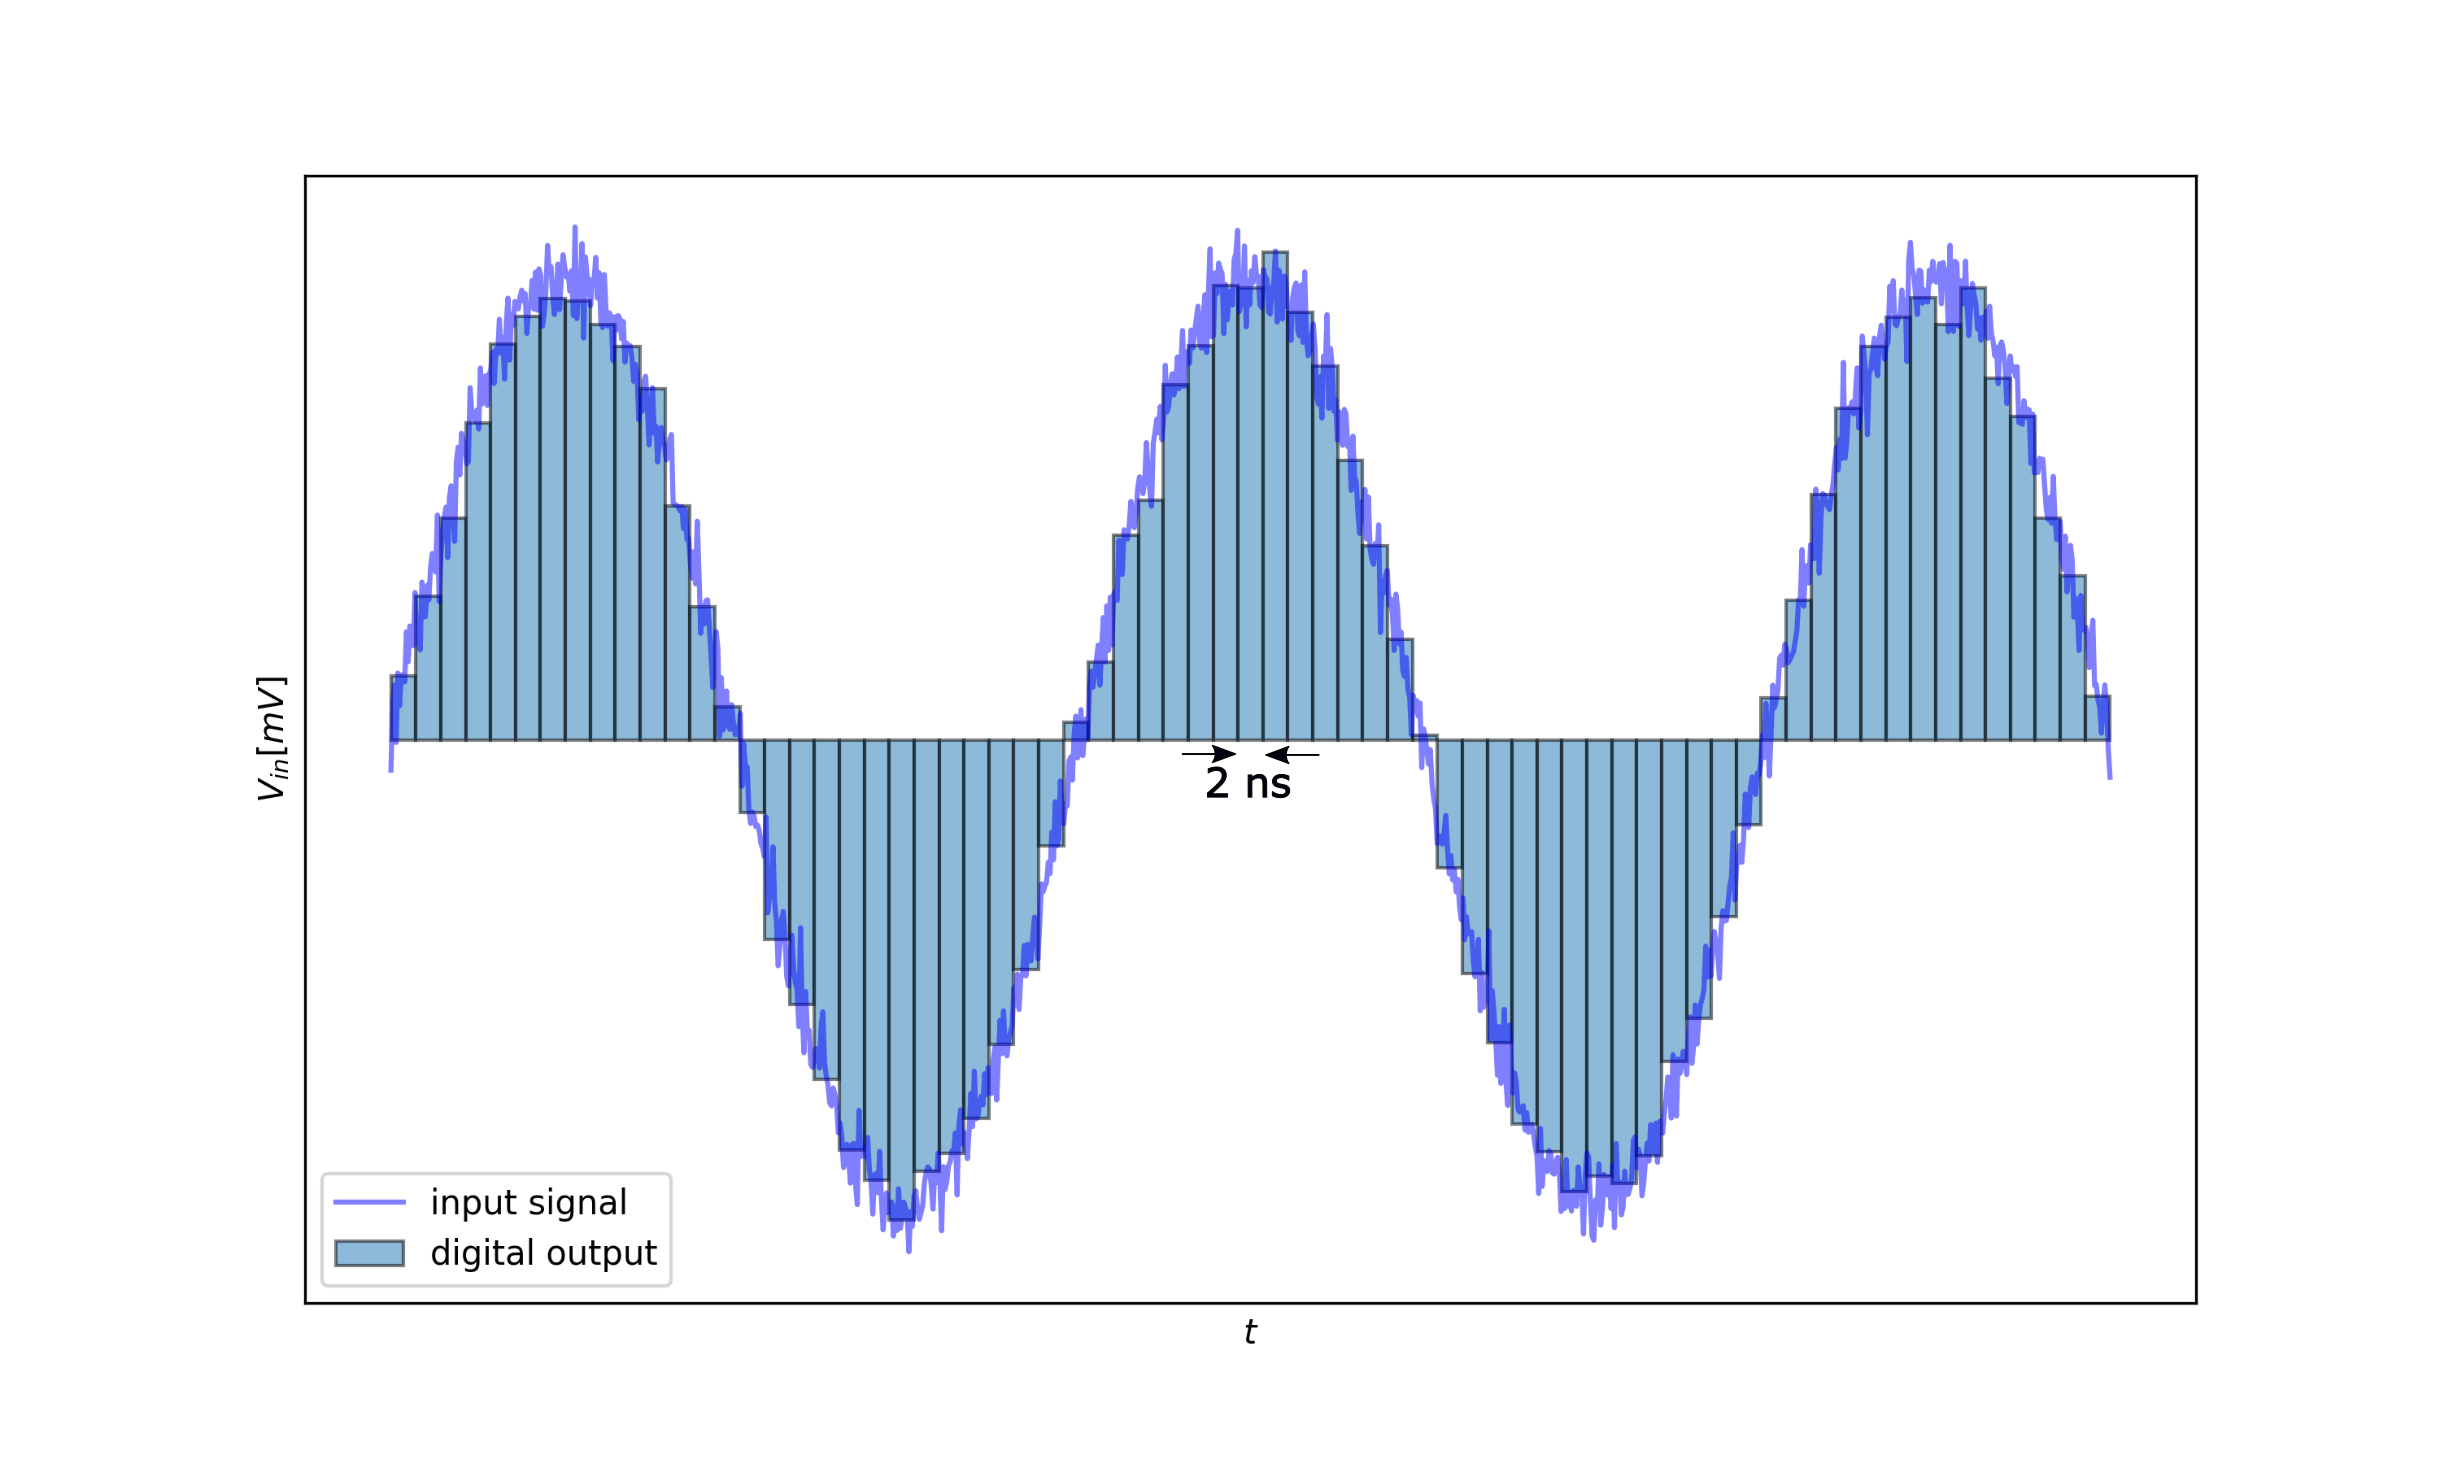
\includegraphics[width=1.0\textwidth]{adc_out.png}
    \caption{Representación de la digitalización a 500 MSPS de una señal proveniente de un sensor. La señal sinusoidal con una componente de ruido representa la señal analógica generada por un sensor, mientras que las barras azul claro dan cuenta de los niveles digitales equivalentes a la señal original con una resolución temporal de 2 ns.}
    \label{fig:adc_out}
\end{figure}

\noindent La resolución del ADC, que se determina por el número de bits del convertidor, afecta directamente a la precisión de estas conversiones. Un número binario con $n$ bits puede representar $2^{n}$ valores. Durante la digitalización, el rango de voltaje desde $V_{\text{min}}$ (usualmente $V_{\text{min}} = 0$) hasta $V_{\text{max}}$ se subdivide en $2^{n} - 1$ intervalos, a cada uno de los cuales se le asigna un valor binario. Si la conversión es lineal, el rango se divide en intervalos de tamaño igual, donde el paso de voltaje más pequeño corresponde al bit menos significativo (LSB, por sus siglas en inglés), que se encuentra más a la derecha en un número binario. En un convertidor analógico-digital (ADC) de $n$ bits, un LSB corresponde a un paso de voltaje de:

\begin{equation}
    1 \text{ LSB} = \frac{V_{\text{max}} - V_{\text{min}}}{2^n - 1}
\end{equation}

\noindent En un ADC ideal, cada conversión de voltaje de entrada a código de salida es independiente, perfectamente lineal y ocurre instantáneamente. Sin embargo, las imperfecciones en los ADCs reales limitan tanto la frecuencia máxima de muestreo como la linealidad y la precisión de la conversión \cite{kolanoski7}.

\subsection{Digital processing}
\label{sec:digital_processing}

\noindent El procesamiento digital de señales (DSP) implica la aplicación de operaciones matemáticas a datos digitales, es decir, números en representación binaria, para analizar, modificar o transformar señales. Este proceso se basa en algoritmos matemáticos que pueden ser implementados en diferentes plataformas de hardware, cada una con sus propias características y ventajas \cite{proakis1}. En la figura \ref{fig:digital_stage} se ilustra un esquema genérico de la etapa de procesamiento digital de señales en un DAQ.\\

\begin{figure}[h]
    \centering
    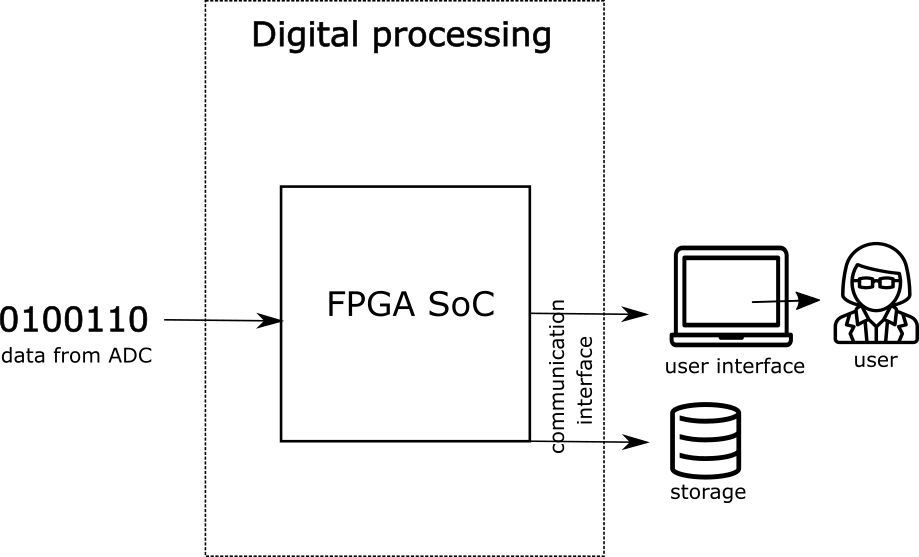
\includegraphics[width=0.6\textwidth]{digital_stage.png}
    \caption{Ilustración de la etapa de procesamiento digital. A la izquierda, los datos provenientes del ADC ingresan al sistema de procesamiento. A continuación, son operados de acuerdo a los algoritmos implementados en el sistema embebido, seguido de la información procesada que se dirige hacia las etapas posteriores de la cadena de información.}
    \label{fig:digital_stage}
\end{figure}

\noindent Las plataformas comunes para el procesamiento digital de señales incluyen varios tipos de sistemas embebidos como microcontroladores ($\mu$Cs), CPUs, FPGAs, GPUs, y DSPs especializados. Cada una de estas plataformas ofrece distintas capacidades en términos de velocidad de procesamiento, latencia, consumo de energía y portabilidad, entre otros factores enumerados a continuación\cite{meyer2007digital}:

\begin{itemize}
    \item  Microcontroladores: Generalmente utilizados para aplicaciones con requisitos de procesamiento relativamente bajos. Ofrecen una buena relación entre costo y funcionalidad, ideal para tareas de procesamiento en tiempo real con bajo consumo de energía.
    \item  CPUs: Adecuadas para aplicaciones que requieren procesamiento general y flexibilidad. Son versátiles y poderosas, pero pueden no ser las mejores para tareas que requieren alta velocidad de procesamiento o baja latencia.
    \item GPUs: Excelentes para el procesamiento paralelo de grandes volúmenes de datos, como en el procesamiento de imágenes o aprendizaje automático. Son capaces de manejar tareas complejas con alta eficiencia, aunque pueden consumir más energía y ser más costosas.
    \item DSPs: Diseñados específicamente para el procesamiento de señales digitales, están optimizados para realizar operaciones matemáticas complejas de manera eficiente. Sin embargo, su producción suele ser costosa debido a su implementación en formato ASIC (Application-Specific Integrated Circuit), lo que puede incrementar el costo total del sistema.
    \item FPGAs: Ofrecen flexibilidad y alta velocidad de procesamiento al permitir la implementación de circuitos personalizados. Son útiles para aplicaciones que requieren procesamiento paralelo o que deben adaptarse a cambios en los requisitos de procesamiento.
\end{itemize}

\subsubsection{Digital processing: Filters}

\noindent Si bien existen diversos tipos de operaciones que se pueden ejecutar en el dominio digital, en el contexto de las señales, las más comunes son los filtros digitales. Estos filtros se utilizan para modificar o extraer información de una señal al atenuar, amplificar o modular ciertas características de la misma, como su amplitud, frecuencia y forma. Los filtros digitales pueden clasificarse en varias categorías, entre ellas \cite{proakis2}:

\begin{itemize}
    \item Filtros FIR (Finite Impulse Response): Estos filtros tienen una respuesta al impulso finita y son conocidos por su estabilidad y capacidad para diseñar respuestas precisas. Son adecuados para aplicaciones donde se requiere un control exacto sobre la respuesta en frecuencia.
    \item Filtros IIR (Infinite Impulse Response): A diferencia de los filtros FIR, los filtros IIR tienen una respuesta al impulso infinita. Estos filtros son generalmente más eficientes en términos de recursos computacionales, pero pueden ser más complejos de diseñar debido a la posibilidad de inestabilidad.
    \item Filtros adaptativos: Estos filtros ajustan sus parámetros en tiempo real para adaptarse a las características cambiantes de la señal o del entorno. Son útiles en aplicaciones donde las condiciones de la señal varían, como en la cancelación de ruido y la ecualización de canales.
    \item  Filtros de paso bajo, paso alto, paso banda y elimina banda: Cada uno de estos filtros está diseñado para permitir o bloquear rangos específicos de frecuencias en una señal. Los filtros de paso bajo permiten pasar frecuencias por debajo de un umbral, mientras que los filtros de paso alto permiten pasar frecuencias por encima de un umbral. Los filtros de paso banda permiten un rango específico de frecuencias y los filtros elimina banda bloquean un rango específico.
\end{itemize}

\noindent Por ejemplo, de acuerdo a \cite{proakis3}, el filtro de media móvil es una técnica fundamental en el procesamiento digital de señales, utilizada para suavizar series temporales de datos. Su objetivo principal es reducir el ruido y las fluctuaciones, proporcionando una estimación más estable y continua de la señal subyacente. Este filtro opera promediando los valores de la señal en una ventana de tiempo móvil. Dependiendo del tipo de media móvil utilizado, este proceso puede implicar el cálculo del promedio simple o ponderado de los valores dentro de la ventana. En este caso, la función de respuesta al impulso \( h[n] \) es una secuencia de valores constantes que suman a uno, específicamente:

\begin{equation}
    h[n] = \frac{1}{N} \cdot \text{rect}\left(\frac{n}{N}\right)
\end{equation}

\noindent donde \( \text{rect} \) es una función rectangular que es 1 dentro del intervalo de la ventana de tamaño \( N \) y 0 fuera de él. Esta respuesta al impulso tiene una longitud de \( N \), que determina el número de muestras de entrada utilizadas para calcular el promedio en cada punto de salida. La salida del filtro de media móvil en tiempo discreto se calcula mediante la convolución de la señal de entrada \( x[n] \) con la función de respuesta al impulso \( h[n] \):

\begin{equation}
    y[n] = (x * h)[n] = \sum_{k=0}^{N-1} x[n-k] \cdot \frac{1}{N}
\end{equation}

\noindent Debido a su respuesta al impulso finita y su implementación directa en términos de convolución, el filtro de media móvil se clasifica como un filtro FIR. Este tipo de filtro es ampliamente utilizado debido a su estabilidad y facilidad de implementación tanto en hardware digital como en software. \\

\noindent El filtro trapezoidal es una herramienta clave en la instrumentación nuclear, especialmente valorada por su capacidad para optimizar la resolución energética en sistemas de adquisición de datos, como aquellos utilizados en detectores de radiación. Este filtro se aplica a la señal de entrada con el objetivo de obtener su amplitud, la cual es proporcional a la energía depositada en el detector. En términos simples, el filtro funciona como un algoritmo que transforma la típica señal de decaimiento exponencial generada por un preamplificador sensible a la carga en una forma trapezoidal. La diferencia de altura entre la línea base de la señal y la parte superior plana del trapezoide refleja la amplitud del pulso inicial, proporcionando una medición directa de la energía del evento. \cite{knoll7}\\

\noindent Además, este filtro tiene la capacidad de mitigar el efecto de pile-up, que ocurre cuando dos o más pulsos de señal se superponen en un corto intervalo de tiempo debido a altas tasas de eventos. Esto provoca la distorsión de los pulsos y deteriora la resolución energética. El filtro trapezoidal, al modificar la forma de los pulsos y reducir su duración, permite distinguir mejor entre eventos consecutivos, minimizando el impacto del pile-up y garantizando mediciones más precisas. Esta capacidad lo convierte en una herramienta fundamental en la instrumentación nuclear y de detección, especialmente en entornos de alta actividad donde la superposición de señales es frecuente.\\

\noindent Es fundamental resaltar que el filtro asume que la señal de entrada se puede aproximar como una función escalón, lo cual es adecuado para modelar los pulsos del preamplificador en términos del tiempo de subida. Sin embargo, esta aproximación no considera el decaimiento natural del pulso. Para corregir este efecto y evitar distorsiones en la medición, se implementa una técnica de corrección polo-cero. Esta técnica ajusta las características del filtro, compensando la caída de la señal y garantizando una mayor precisión en la determinación de la energía.\\

\noindent El filtro trapezoidal digital se basa en un algoritmo recursivo que convierte un pulso exponencial digitalizado \( v(n) \) en un pulso trapezoidal simétrico \( s(n) \) \cite{jordanov1994digital}. El proceso comienza con el cálculo de \( d^{k,l}(n) \), una combinación de diferencias de muestras de la señal \( v(n) \) en distintos momentos del tiempo. Esta fórmula resta valores de \( v(n) \) separados por \( k \) y \( l \) muestras para obtener la diferencia temporal de la señal:

\begin{equation}
d^{k,l}(n) = v(n) - v(n-k) - v(n-l) + v(n-k-l)
\end{equation}

\noindent Posteriormente, las siguientes ecuaciones definen cómo se calcula el pulso resultante \( s(n) \) en función de las sumas acumuladas de \( d^{k,l}(n) \), lo que genera una forma trapezoidal. Los valores iniciales de \( p(n) \), \( r(n) \) y \( s(n) \) son iguales a cero para \( n < 0 \).

\begin{equation}
p(n) = p(n-1) + d^{k,l}(n), \quad n \geq 0
\end{equation}

\begin{equation}
r(n) = p(n) + M \cdot d^{k,l}(n)
\end{equation}

\begin{equation}
s(n) = s(n-1) + r(n), \quad n \geq 0
\end{equation}

\noindent donde \( p(n) \), \( r(n) \) y \( s(n) \) son las variables acumuladas. El parámetro \( M \) depende del tiempo de decaimiento \( \tau \) del pulso exponencial y del período de muestreo \( T_{clk} \), y se define como:

\begin{equation}
M = \frac{1}{\exp\left(\frac{T_{clk}}{\tau}\right) - 1}
\end{equation}

\noindent Cuando \( \frac{\tau}{T_{clk}} > 5 \), \( M \) puede aproximarse como:

$$
M \approx \frac{\tau}{T_{clk}} - 0.5
$$

\noindent El cálculo de \( d^{k,l}(n) \) se puede expresar mediante dos procedimientos secuenciales:

\begin{equation}
d^{k}(n) = v(n) - v(n-k)
\end{equation}

\begin{equation}
d^{k,l}(n) = d^{k}(n) - d^{k}(n-l)
\end{equation}

\noindent Este algoritmo implementa de manera eficiente la conversión de un pulso exponencial en una señal trapezoidal, mejorando la precisión en la medición de la energía del evento detectado al eliminar ruido de alta frecuencia y adaptar la forma de la señal para su procesamiento digital.\\

\noindent Además de los filtros para señales, otros subsistemas de procesamiento pueden implementarse en la etapa de procesamiento digital. Ejemplos de estos incluyen los sistemas de trigger, que generan una señal digital en respuesta a eventos específicos, activando acciones en otras etapas del sistema de adquisición o en sistemas de adquisición conectados y son esenciales en experimentos de detección de partículas. Del mismo modo, en el contexto de la instrumentación científica para mediciones de radiación, se encuentran sistemas digitales complejos de gran utilidad para extraer información física de interés como son:

\begin{itemize}
    \item Analizador de Canal Único (SCA): Se emite una señal digital si la señal de energía está entre un rango de canales designado por un Discriminador de Nivel Inferior (LLD) y un Discriminador de Nivel Superior (ULD). Normalmente se muestra el número de cuentas por segundo \cite{knoll5}.

    \item Escalado Multicanal (MCS): Similar al modo SCA, pero los datos se registran en un histograma de tiempo, en el que se registran sucesivas tasas de conteo \cite{knoll8}.
    
    \item Analizador de Altura de Pulso (PHA): También conocido como MCA, las energías se registran en un histograma de energía, en el que las alturas de los pulsos se categorizan por canal, y el número en cada canal representa la cantidad de veces que se registró una altura de pulso particular durante el tiempo de medición \cite{knoll6}.
    
    \item Escalado Multiespectral (MSS): Similar al modo PHA, pero se guarda un histograma de energía en intervalos de tiempo cortos, definidos por el tiempo de residencia del sistema\cite{knoll8}.
    
    \item Modo de Lista con Marca de Tiempo (TLIST): En este modo, se registra el momento en que ocurre un evento, con una precisión de hasta 100 ns, junto con la energía del evento. Estos datos se almacenan como una lista de pares tiempo-energía, que luego pueden procesarse en cualquiera de los cuatro tipos de datos mencionados anteriormente. Aunque esta es la opción más general de almacenamiento de datos, también es la que utiliza la mayor cantidad de memoria \cite{burnett2019time}.
\end{itemize}

\noindent Como se ha mencionado anteriormente, diversas plataformas de hardware pueden utilizarse para aplicaciones de procesamiento digital, incluidos los ejemplos presentados. Sin embargo, es fundamental identificar los requerimientos específicos de cada aplicación para lograr una implementación eficiente. Por ejemplo, un microcontrolador de bajo costo como el ESP32 puede emplearse para desarrollar un PHA, como el descrito por \cite{ramirez2024}. No obstante, esta implementación enfrenta limitaciones inherentes a la lógica secuencial de los microcontroladores, lo que implica que la lectura de los canales de altura se realice de manera secuencial. Esto puede resultar en la pérdida de eventos en los canales que no se están leyendo en un momento dado, especialmente si la frecuencia de generación de eventos es alta en comparación con el tiempo de muestreo. Esta situación pone de manifiesto la necesidad de realizar la lectura de los canales de altura de forma simultánea, lo que requiere un sistema de procesamiento con capacidad de paralelización y, en consecuencia, la necesidad de utilizar plataformas de hardware más avanzadas.\\

\noindent Con esto presente y dada la necesidad de procesar grandes volúmenes de datos generados por ADCs de alta velocidad mientras se minimiza la latencia, para el desarrollo de DAQs de alto rendimiento, se hace imprescindible la implementación de sistemas de procesamiento basados en FPGA. Además, esta tecnología permite la evolución continua de los sistemas digitales gracias a su capacidad de reconfiguración.

\subsubsection{Digital Processing: FPGA}
\noindent Una FPGA es un tipo de circuito integrado reconfigurable que permite a los usuarios personalizar su arquitectura interna para realizar tareas específicas, diferenciándose de los microprocesadores tradicionales, que operan con un conjunto de instrucciones fijas. Estas matrices de puertas programables en campo son ampliamente utilizadas en aplicaciones que requieren procesamiento en paralelo y alta flexibilidad, como en sistemas de telecomunicaciones y procesamiento de señales digitales. La capacidad de reprogramación de las FPGA les otorga una ventaja significativa en términos de adaptabilidad a nuevas necesidades sin requerir modificaciones físicas en el hardware. Para programar una FPGA, se utilizan lenguajes de descripción de hardware (HDL) como VHDL o Verilog, que permiten definir circuitos personalizados que se cargan directamente en el dispositivo, configurando su comportamiento según el diseño especificado \cite{brown2000fundamentals}.\\

\noindent Como se ilustra en la figura \ref{fig:fpga_arch}, internamente una FPGA se compone de una matriz de bloques lógicos programables (CLBs), interconexiones configurables, y recursos adicionales como bloques de memoria (BRAM). Los CLBs contienen LUTs (Look-Up Tables) y flip-flops, que implementan funciones lógicas y almacenan estados. Las interconexiones programables permiten la comunicación entre los bloques lógicos a través de una red de enrutamiento configurable. Además, suelen incluir bloques dedicados para funciones específicas, como multiplexores y controladores de entrada/salida, lo que proporciona una gran flexibilidad y capacidad de adaptación a distintas aplicaciones \cite{bravo2020new}.\\

\begin{figure}[h]
    \centering
    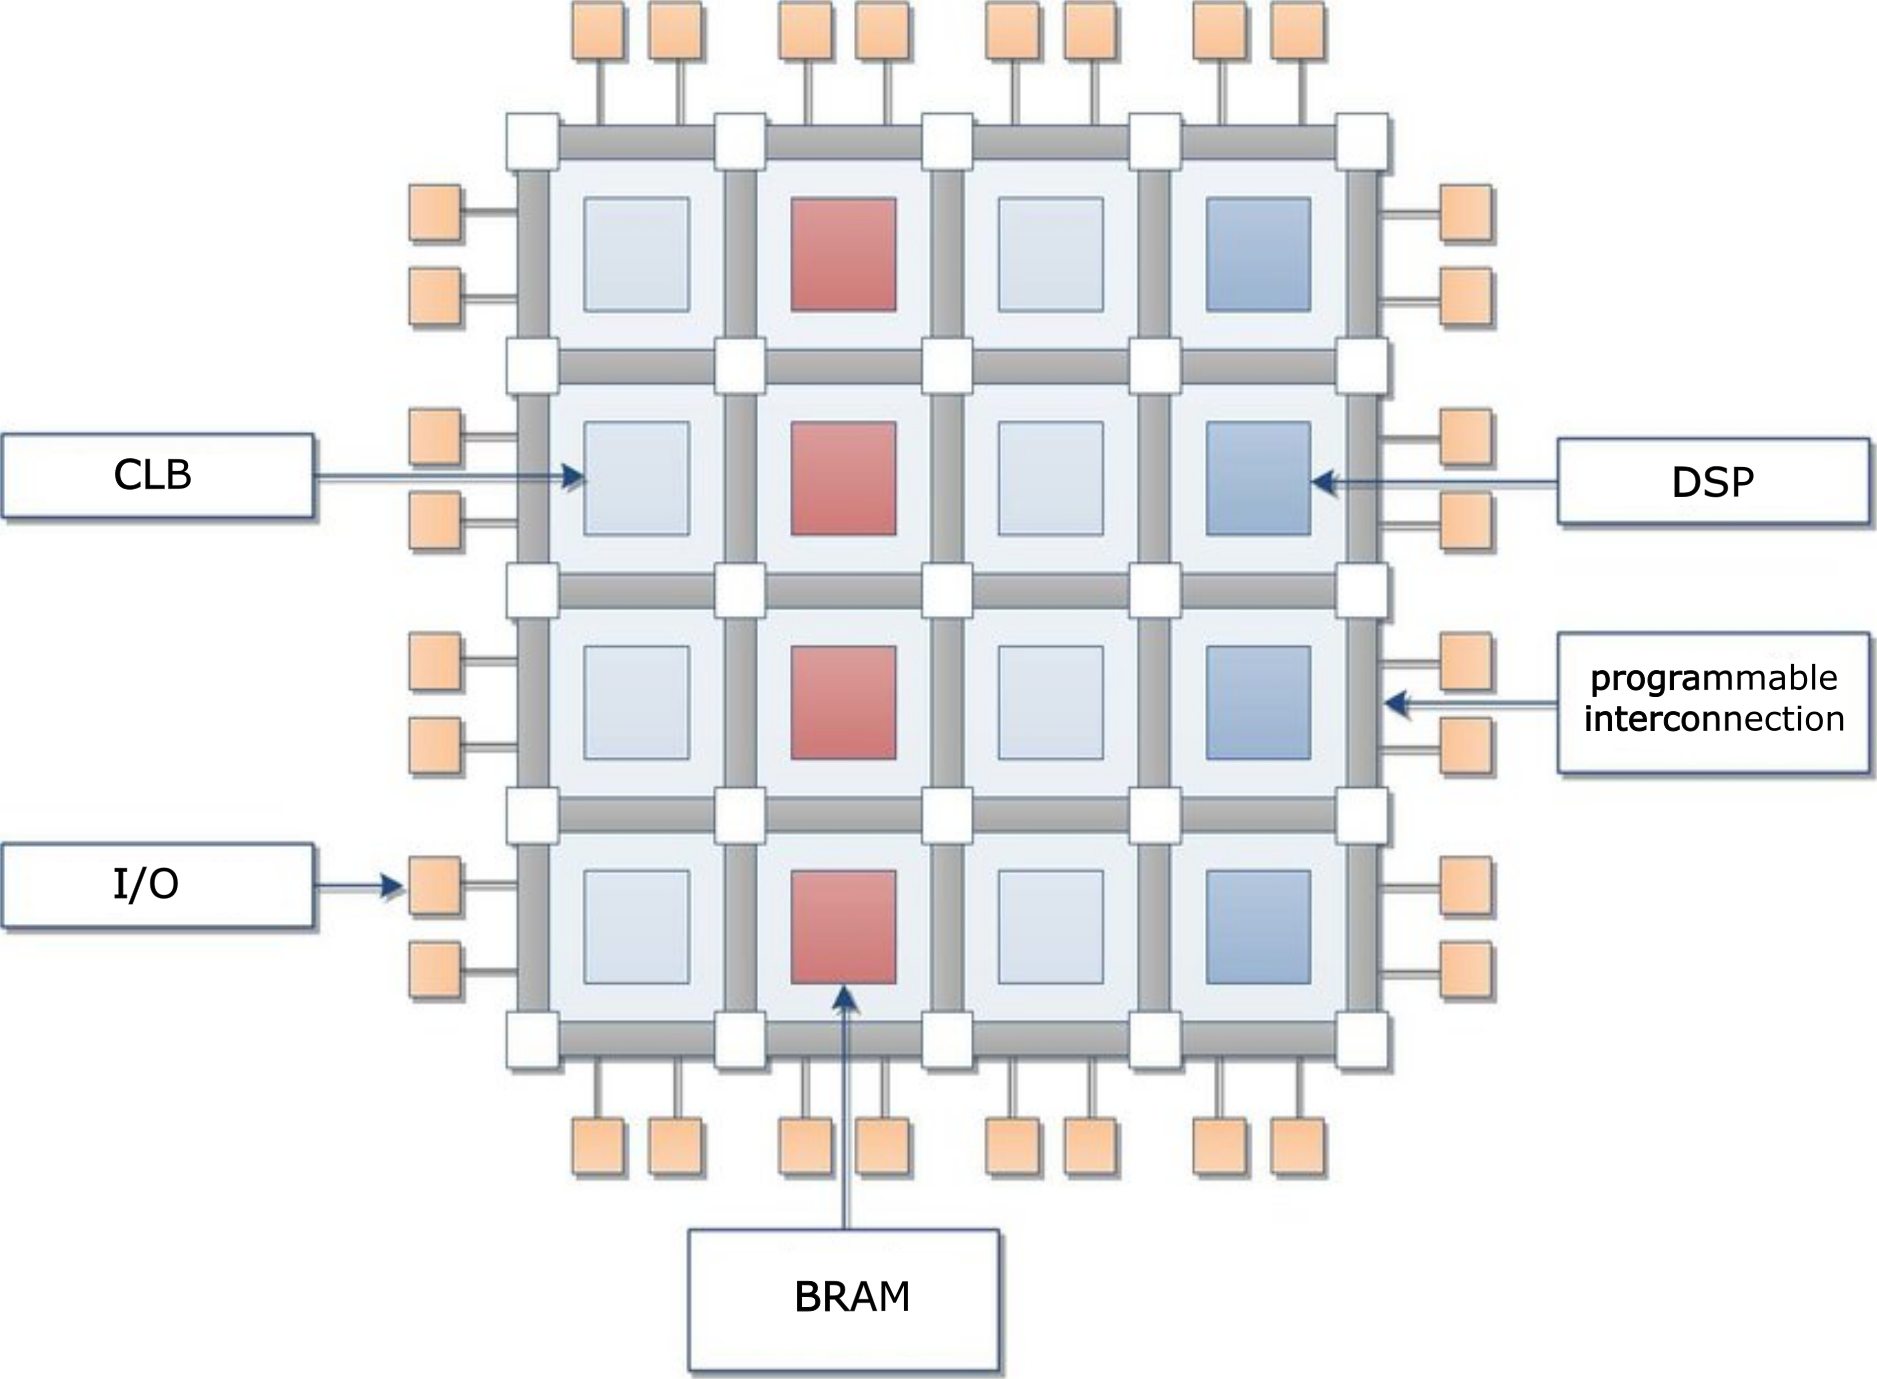
\includegraphics[width=0.6\textwidth]{fpga_arch.png}
    \caption{Diagrama de la arquitectura típica de una FPGA. En este se pueden observar las partes fundamentales del dispositivo como los CLBs, puertos de entrada y salida I/O, módulos de BRAM, etapas dedicadas al procesamiento de señales DSP y las interconexiones programables. Tomado de \cite{Rucci2018heterogeneos}.}
    \label{fig:fpga_arch}
\end{figure}

\noindent Esta arquitectura ofrece baja latencia, lo cual es esencial para manejar el gran volumen de datos generado por ADCs de alta velocidad. Su capacidad de procesamiento paralelo permite gestionar eficientemente altas tasas de muestreo, asegurando un procesamiento de datos proveniente de sistemas de sensado sin pérdida de información. En particular, las FPGA ofrecen una flexibilidad considerable en el diseño e implementación de algoritmos de procesamiento de señales, incorporando módulos de hardware dedicados como los DSPs (Digital Signal Processors) \cite{meyer2007digital}.\\

\subsubsection{Digital processing: FPGA SoC}

\noindent No obstante, como señala Bravo \cite{bravo2020new}, los avances en tecnología FPGA han impulsado el desarrollo de sistemas híbridos, como los SoC (System on Chip). Según el fabricante AMD \cite{amd_zynq_7000}, un FPGA SoC es un dispositivo que integra en un solo chip la flexibilidad programable de una FPGA, también conocida como Lógica Programable (PL, por sus siglas en inglés), con las capacidades de procesamiento de un sistema basado en un procesador (PS, Processing System), generalmente de arquitectura ARM. Como se muestra en la figura \ref{fig:fpga_soc}, existe un subsistema de intercomunicación o bus entre el PS y el PL, donde típicamente el PS actúa como maestro y el PL como esclavo. \\

\begin{figure}[h]
    \centering
    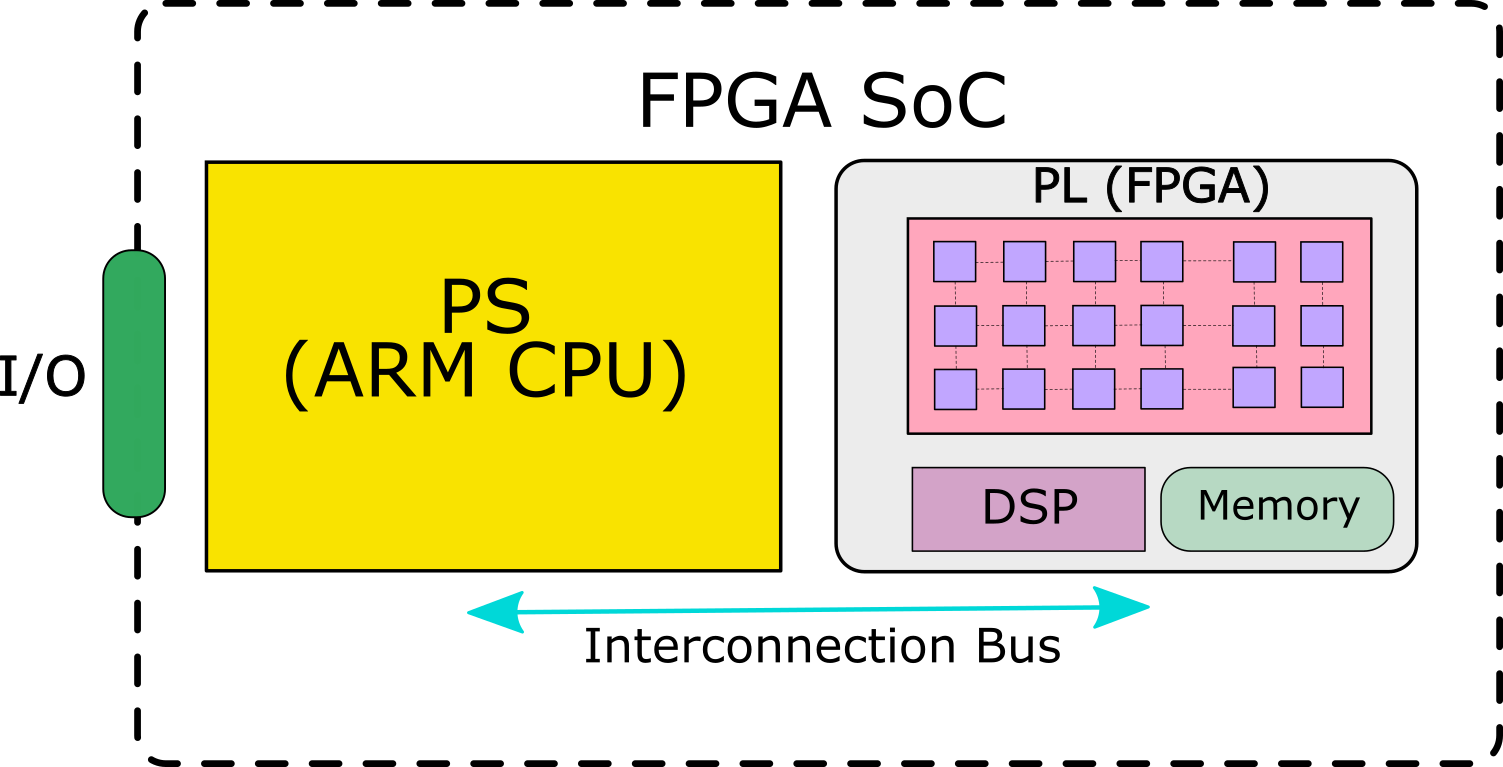
\includegraphics[width=0.6\textwidth]{FPGA_SoC.png}
    \caption{Arquitectura típica de un FPGA SoC. En su estructura fundamental se aprecia el procesador (PS), la FPGA (PL) y el bus de interconexión entre estos dos.}
    \label{fig:fpga_soc}

\end{figure}

\noindent Esta configuración permite aprovechar lo mejor de ambos mundos: la capacidad de realizar tareas complejas y variables mediante software y, al mismo tiempo, la ejecución de operaciones intensivas en paralelo y en tiempo real mediante la lógica programable de la FPGA. Además, esta integración incluye funcionalidades adicionales como procesamiento digital de señales (DSP), dispositivos de señal mixta, y la posibilidad de reemplazar otros componentes dedicados como los ASICs (Application-Specific Integrated Circuits) o ASSPs (Application-Specific Standard Products), todo en un solo dispositivo, optimizando así el rendimiento y la eficiencia energética para aplicaciones específicas.\\

\noindent Es importante destacar las interfaces de memoria disponibles en estos dispositivos. Las FPGA suelen integrar varios bloques de memoria, como registros, RAM y FIFOs, cada uno con funciones específicas. Los registros son pequeños bloques de memoria que almacenan datos temporales para operaciones inmediatas, lo que permite un acceso rápido y eficiente. La RAM (Memoria de Acceso Aleatorio) se utiliza para el almacenamiento de datos volátiles, ofreciendo mayor capacidad que los registros, pero con tiempos de acceso más largos. Las FIFOs (Colas de Primeros en Entrar, Primeros en Salir) son estructuras de almacenamiento que gestionan flujos de datos de manera ordenada, lo que resulta fundamental para el procesamiento secuencial y la sincronización entre diferentes módulos \cite{bravo2020new}. Por su parte, el procesador tiene acceso a estos recursos de memoria y periféricos a través de la interfaz DMA (Direct Memory Access), permitiendo la administración de los datos almacenados en las memorias de la FPGA a través del bus de intercomunicación. De esta manera, el PS ofrece al usuario la capacidad de acceder, modificar o extraer estos recursos de memoria, facilitando la adquisición de datos y el control de manera efectiva.\\

\noindent Debido a la naturaleza de los SoC FPGA, estos no cuentan con un conjunto de instrucciones predefinido de fábrica. Para implementar aplicaciones en esta tecnología, es necesario diseñar circuitos lógicos y desarrollar algoritmos que configuren y controlen la plataforma de acuerdo a los requerimientos específicos del proyecto. En arquitecturas de sistemas de adquisición de datos (DAQs) de alto rendimiento, especialmente en el contexto de la detección de partículas, es común dividir las funciones en "fast control" y "slow control" \cite{kolanoski8}. El "fast control", generalmente implementado en FPGA, gestiona procesos de alta velocidad y tiempo real, como el procesamiento digital de señales en pipeline, mientras que el "slow control", basado típicamente en plataformas de microprocesadores, se encarga de los algoritmos de supervisión del sistema. La tecnología SoC con FPGA permite integrar ambas funciones en un solo hardware, distribuyendo la lógica de fast control en el PL y los algoritmos de supervisión de niveles de voltaje, gestión de comunicaciones y acceso a memoria en el PS.

\subsection{Communication interface}
\label{sec:communication_interface}

\noindent Si bien las plataformas mencionadas pueden realizar operaciones en línea, procesando las señales a medida que ingresan al sistema, es esencial enviar la información a etapas externas del sistema de adquisición de datos (DAQ) para realizar actividades adicionales, como almacenamiento, posprocesamiento, interacción con otros sistemas de detección (como triggers) y transferencia a interfaces de alto nivel de abstracción, como computadoras de escritorio, para que el usuario pueda acceder a los datos. La etapa encargada de dicha transferencia es la interfaz de comunicación. \\

\noindent Es importante señalar que la mayoría de la tecnología de comunicaciones se basa en señales digitales, es decir, en la manipulación de bits (1s y 0s). Esto implica que el sistema de procesamiento digital debe implementar un conjunto de instrucciones en forma de algoritmos o subsistemas para codificar la información procesada en un formato específico, asegurando así una transmisión efectiva. Además, la interfaz de comunicaciones se compone principalmente de un estándar de hardware y un protocolo digital particular y dependiendo de la complejidad de la aplicación y del DAQ, se pueden emplear diferentes tipos. Algunos ejemplos de estos protocolos, que abarcan desde tecnología de consumo hasta grandes sistemas de servidores, incluyen: RS-232, RS-485, USB, GPIB, Ethernet, Wi-Fi, Modbus/TCP, CAN Bus, Profibus, Profinet, SCADA, EtherCAT, MMS, MQTT, OPC UA, LHC Computing Grid e INFN-Tier-1 \cite{zurawski2014industrial} \cite{bortolotti2012infn}.\\

\noindent Aunque las comunicaciones paralelas fueron comunes en el pasado, su implementación en largas distancias se ha vuelto impráctica debido a la necesidad de una línea de transmisión para cada bit de información, lo que incrementa la complejidad, el costo y los riesgos de interferencia y desincronización. Por esta razón, la mayoría de las interfaces de comunicación alámbricas modernas son de tipo serial. Las interfaces seriales, como USB, Ethernet y UART, permiten la transmisión de datos a altas velocidades utilizando solo unas pocas líneas, lo que las hace más eficientes, fiables y económicas para una amplia gama de aplicaciones, desde sistemas de adquisición de datos hasta comunicaciones en redes de larga distancia \cite{eeeguide_serial_communication_8251}.\\

\noindent En términos generales, la transmisión de datos en serie se puede clasificar según la manera en que se realiza la transmisión:
 \begin{itemize}
    \item Simplex: el hardware está diseñado de manera que la transferencia de datos ocurre únicamente en una dirección. No es posible transferir datos en la dirección opuesta. Un ejemplo típico es la transmisión desde una computadora hacia una impresora.
    \item Half Duplex: La transmisión half duplex permite la transferencia de datos en ambas direcciones, pero no de manera simultánea. Un ejemplo común es el uso de un walkie-talkie.
    \item Full Duplex: La transmisión full duplex permite la transferencia de datos en ambas direcciones de manera simultánea. Un ejemplo típico son las líneas telefónicas.
 \end{itemize}

 \noindent Es importante destacar que, aunque hasta ahora se ha presentado el concepto de DAQ como un sistema en el que la información fluye desde el sistema físico hacia el usuario, como se ilustra en la figura \ref{fig:DAQ_generic}, en la mayoría de los dispositivos o instrumentos de medición es común que también exista un flujo de información en la dirección opuesta. Este subsistema, conocido como sistema de control, abarca todas las acciones que el usuario puede realizar para configurar parámetros en el sistema, ya sea para controlar actuadores o para modificar modos de operación en cualquiera de las etapas descritas. En los dispositivos que cuentan con esta funcionalidad, es crucial disponer de interfaces de comunicación half duplex o full duplex, que permitan la modificación de parámetros en el sistema de manera simultánea al flujo de información de medición.\\

 \noindent De acuerdo con \cite{eeeguide_serial_communication_8251}, los datos en la interfaz de comunicación en serie pueden enviarse en dos formatos principales: asíncrono y síncrono. En el formato asíncrono, orientado a caracteres, los bits de un carácter o palabra de datos se envían a una tasa constante. Sin embargo, los caracteres pueden llegar a cualquier ritmo (asíncronamente), siempre que no se solapen. Durante los períodos en que no se envían caracteres, una línea se mantiene en nivel alto (lógica 1), conocido como "mark" (marca), mientras que la lógica 0 se denomina "space" (espacio). El inicio de un carácter se señala mediante un bit de inicio, que siempre es bajo, y se utiliza para sincronizar el transmisor con el receptor. Después del bit de inicio, se envían los bits de datos comenzando por el bit menos significativo, seguido de uno o más bits de parada, que son activos en alto y marcan el final del carácter. Dependiendo del sistema, se pueden utilizar 1, 1 1/2 o 2 bits de parada. La combinación del bit de inicio, el carácter y los bits de parada se conoce como "frame" (trama). Aunque los bits de inicio y de parada no transportan información útil, son esenciales debido a la naturaleza asíncrona de la transmisión de datos. Además, la tasa de transmisión puede expresarse en bits por segundo (bits/seg) o caracteres por segundo (caracteres/seg), siendo el término bits/seg también conocido como la tasa de baudios. Este formato asíncrono es comúnmente utilizado en transmisiones de baja velocidad, típicamente menores a 20 Kbits/seg.\\

\noindent Por otro lado, los bits de inicio y de parada en cada trama del formato asíncrono representan bytes de sobrecarga que reducen la tasa general de caracteres. Estos bits de inicio y parada pueden eliminarse al sincronizar el receptor y el transmisor, la cual se puede lograr mediante una señal de reloj común.\\

\noindent Independientemente de si el dispositivo receptor de la información del DAQ es una computadora de escritorio o un clúster de servidores, es crucial contar con un método sistemático para la decodificación de los datos. Usualmente, se diseñan programas informáticos con algoritmos específicos para reorganizar la información que llega empaquetada en formatos definidos por el protocolo utilizado. Este software actúa como una capa de primer nivel en la gestión de la información proveniente del DAQ y debe integrarse con otros programas para transferir los datos a capas de abstracción que permitan al usuario acceder a la información relevante adquirida por el sistema. Este tipo de software, comúnmente conocido como controlador de comunicaciones, debe ser instalado o implementado junto con otros controladores del DAQ en el dispositivo de recepción.\\

\noindent Para ilustrar el uso de las interfaces de comunicación en la instrumentación científica y los sistemas de adquisición de datos (DAQs), consideremos dos instrumentos de medición con diferentes requerimientos y niveles de complejidad: un sistema de monitoreo de temperatura ambiental y un sistema de detección de partículas radiactivas en una central nuclear. En el primer caso, dado que las variaciones de temperatura debidas a cambios ambientales ocurren en un orden temporal de minutos o incluso horas, es suficiente adquirir las señales del sensor de temperatura con una granularidad de segundos, lo que corresponde a una frecuencia de muestreo del orden de los Hz. Esto permite implementar una plataforma de procesamiento digital de bajo rendimiento, como un microcontrolador de bajo consumo, similar a los utilizados en tarjetas de desarrollo como Arduino. En consecuencia, la interfaz de usuario podría ser un bus serial USB, fácilmente configurado en el microcontrolador y conectado a un ordenador. Con un software simple, los datos pueden ser decodificados y representados en una interfaz de usuario, permitiendo el análisis de los cambios de temperatura ambiental, que es el objetivo de esta aplicación. \\

\noindent Por otro lado, en el caso de un sistema de detección de radiación, no solo es posible que las tasas de generación de eventos alcancen el orden de los kHz, sino que los eventos individuales pueden durar del orden de $\mu$s o incluso ns, dependiendo del tipo de detector \cite{knoll9}. Estas características exigen que el sistema de digitalización, el procesamiento digital, y la correspondiente interfaz de comunicaciones tengan un rendimiento significativamente superior al del ejemplo anterior. En este caso, es probable que un bus de comunicación serial USB se sature, lo que resultaría en la pérdida de información valiosa debido a la latencia de la interfaz. Por lo tanto, sería necesario considerar interfaces diseñadas para gestionar y transmitir grandes volúmenes de datos, como Ethernet. Si además se garantiza que el dispositivo receptor, como un ordenador, cuenta con el software adecuado para administrar y decodificar la información proveniente de la interfaz Ethernet, se podrá representar la información de manera útil para el usuario, por ejemplo, como un espectro de energías de la fuente radiactiva.


% \subsection{Procesamiento Digital de Pulsos}
 
% \noindent Como se explicó en el apartado de electrónica de front-end, los filtros analógicos suelen aplicar una combinación de diferenciaciones e integraciones de la forma de onda de voltaje para transformarla en una forma similar a la de una gaussiana, cuya amplitud es proporcional al voltaje $V$ y, por lo tanto, a la energía de la radiación. Sin embargo, de acuerdo a \cite{loudenuclearspectroscopy}, en el enfoque digital, tras la digitalización de la señal utilizando un ADC, se aplica un filtro matemático a esta serie de valores digitales para eliminar los componentes de ruido de alta frecuencia, mejorando así la SNR y determinando la amplitud de voltaje $V$.\\

% \noindent Este enfoque presenta ventajas significativas en comparación con el procesamiento de señales analógicas tradicional, entre las cuales destacan \cite{radeka1968optimum}:

% \begin{itemize}
%     \item Aplicación de análisis considerando diferencias pulso a pulso: Permite analizar cada pulso individualmente, teniendo en cuenta sus particularidades.
%     \item Análisis de señales de carga inducida transitoria: Facilita la interpretación de señales transitorias que pueden ser difíciles de captar con métodos analógicos.
%     \item  Mejora del parámetro de tiempo muerto: Reduce las limitaciones temporales que pueden afectar la adquisición continua de señales.
%     \item Captura fácil de señales, incluida la implementación de análisis complejos: Simplifica la adquisición de datos y permite realizar análisis detallados y sofisticados.
%     \item Procesamiento de señales con criterios basados en coincidencias (diferentes detectores o diferentes partes del mismo detector): Facilita la correlación de eventos entre múltiples detectores o áreas de un detector.
%     \item Aplicación efectiva de post-procesamiento de datos: Permite el pre-análisis de formas de onda, modelado de pulsos y verificación de algoritmos de deconvolución de superposición de pulsos (pulse pile-up).

% \end{itemize}

% \noindent La implementación de procesadores digitales de pulsos (DPP) en FPGA, gracias a su riqueza en recursos lógicos digitales, les permite soportar múltiples modos de adquisición, como análisis de altura de pulso, escalado de canales múltiples, escalado de espectros múltiples y adquisición en modo de lista con marcas de tiempo. Además, ofrecen funcionalidades muy especializadas como discriminación y corrección de la forma del pulso, rechazo de superposición de pulsos (pulse pile-up), conteo sin pérdidas y otras características que respaldan la medición. Adicionalmente, múltiples DPP pueden operar de manera sincronizada para permitir la correlación temporal de eventos provenientes de múltiples fuentes de señal, como detectores separados o segmentos de un mismo detector. \\

% \noindent En el capítulo System, se desarrolla la aplicación de los conceptos expuestos en este capítulo, en un sistema experimental de lectura y procesamiento para detectores GEM.

% \noindent Como se expuso anteriormente, los electrones multiplicados son recogidos en los electrodos de salida del GEM, resultando una señal de corriente eléctrica que puede ser medida y analizada. Dependiendo de los objetivos del experimento, distintas etapas electrónicas pueden ser implementadas a continuación. Sin embargo, el objetivo de estas converge a preservar y transportar la información física de interés contenida en la señal, optmizando factores clave como \cite{knoll2010radiation}:

% \begin{itemize}
%     \item Supresión de ruido 
%     \item Reducción del tiempo muerto
%     \item Reducción del déficit balístico para mejorar la resolución y reducir la distorsión de los picos
% \end{itemize}

% \noindent Aunque los distintos tipos de detectores generan señales eléctricas únicas, dependiendo de los procesos físicos que ocurren en su interior, es posible identificar características comunes que facilitan la comprensión de conceptos clave en el acondicionamiento y procesamiento de señales.

%Particularmente en la medición de eventos propios de cor´pusculos, se presentan señales de tipo pulsado...
\subsection{User interface}

\noindent La interfaz de usuario en un sistema de adquisición de datos (DAQ) es un componente clave que conecta al operador con el sistema de control y análisis de datos. Esta interfaz puede ser tan simple como una terminal de comandos, también conocida como interfaz de línea de comandos (CLI), donde el usuario interactúa mediante instrucciones textuales, o bien, puede adoptar un enfoque más sofisticado mediante una interfaz gráfica de usuario (GUI) \cite{webster1}.\\

\noindent Mientras que una CLI ofrece control directo y a menudo preciso mediante comandos específicos, las GUI están diseñadas para ser más intuitivas y accesibles, permitiendo a los usuarios interactuar con el sistema a través de elementos gráficos como botones, menús y ventanas. Las GUI son particularmente útiles cuando se requiere visualizar grandes volúmenes de datos o realizar configuraciones complejas de manera visual.\\

\noindent La función principal de estas interfaces, en especial de una GUI, es representar la información física adquirida por el sistema de manera lógica y sistemática, basada en las variables físicas estudiadas. A través de tablas, gráficos estáticos o dinámicos que se actualizan en tiempo real, o histogramas que permiten visualizar distribuciones de datos, la interfaz facilita el análisis de los resultados obtenidos. Estas representaciones visuales permiten a los usuarios interpretar rápidamente el comportamiento del sistema físico bajo estudio, detectando tendencias, anomalías o eventos significativos de forma eficiente.\\

\noindent Además de la representación de los datos, tanto las CLI como las GUI permiten al usuario controlar y configurar las diferentes etapas del DAQ. En una CLI, esto se realiza a través de comandos textuales, mientras que en una GUI se logra mediante recursos gráficos como botones, deslizadores o menús desplegables. Estas opciones de control permiten ajustar parámetros críticos, como la frecuencia de muestreo, los umbrales de detección o la selección de canales de adquisición, lo que otorga al usuario flexibilidad para adaptar el sistema a los requisitos específicos de la aplicación.\\

\noindent La importancia de esta etapa radica en que una interfaz bien diseñada no solo mejora la experiencia del usuario, sino que también maximiza la eficiencia y precisión del sistema. Un diseño intuitivo reduce la posibilidad de errores, simplifica el acceso a configuraciones avanzadas y optimiza el flujo de trabajo del investigador. Las GUI, en particular, permiten una mayor interacción y manipulación en tiempo real de los datos, lo cual es crítico en experimentos que requieren monitoreo constante y ajustes inmediatos.\\

\noindent En el ámbito de la instrumentación científica, la GUI también juega un papel crucial al proporcionar al usuario herramientas de análisis visuales y personalizables. A través de estas interfaces, es posible profundizar en los datos adquiridos, identificar patrones o irregularidades, y generar reportes gráficos que faciliten la toma de decisiones experimentales. Las opciones avanzadas de automatización, como la capacidad de definir secuencias de comandos o macros, permiten al usuario programar el DAQ para realizar tareas específicas de manera automática, lo que es especialmente útil en experimentos de larga duración o con grandes volúmenes de datos.

\newpage 

\section{Metodología y montaje experimental}

\noindent Este trabajo presenta la implementación de un sistema de adquisición de datos (DAQ) monocanal de alto rendimiento, que integra una etapa de digitalización de alta velocidad, un sistema de procesamiento digital basado en FPGA SoC, una interfaz de comunicación de alta capacidad y una interfaz de usuario desarrollada en Python para la visualización y control de datos. La arquitectura está optimizada para adquirir de manera eficiente señales procedentes de diversos sistemas de sensado, complementados por su correspondiente electrónica de acondicionamiento. Además, el sistema es altamente adaptable a una amplia variedad de aplicaciones, que abarcan desde el ámbito biomédico hasta la detección de partículas subatómicas. En este trabajo, sin embargo, se emplea un generador de señales para validar su funcionamiento.\\

\noindent A continuación, se describe la metodología de implementación, que incluye el hardware utilizado, los módulos de adquisición y procesamiento de señales configurados en el PL o FPGA, y el bloque de comunicaciones ComBlock, que permite el acceso a la memoria desde el PS. También se detalla la configuración de la interfaz de comunicaciones entre el PS y el usuario, denominada UDMA, y la implementación del software de control en Python, que actúa como interfaz de usuario.\\

% Tanto el hardware utilizado como la metodología de trabajo se fundamentan en los resultados obtenidos en la escuela conjunta ICTP-IAEA sobre aplicaciones de instrumentación científica y nuclear basadas en FPGA SoC \cite{ictp_smr3765}.

%\subsection{Montaje experimental: Digitalization hardware - ADC500}

\noindent Se utiliza el instrumento Digilent Analog Discovery 2 (AD2) (fig. \ref{fig:AD2}) como generador de señales, aprovechando la versatilidad de este dispositivo multifuncional, que también incluye un osciloscopio, una fuente de poder regulable y un analizador lógico, entre otros instrumentos integrados. El AD2 no solo permite acceder a funciones predefinidas, sino que también facilita la programación de formas de señal personalizadas e incluso la creación manual de estas a través de la interfaz gráfica de su software de control, WaveForms (fig. \ref{fig:wf_setup}). Además, ofrece la opción de añadir ruido y otras características que permiten la generación de señales sintéticas, emulando la respuesta real de sensores o detectores, lo cual es fundamental para la validación del sistema de adquisición de datos (DAQ) implementado.

\begin{figure}[H]
    \centering
    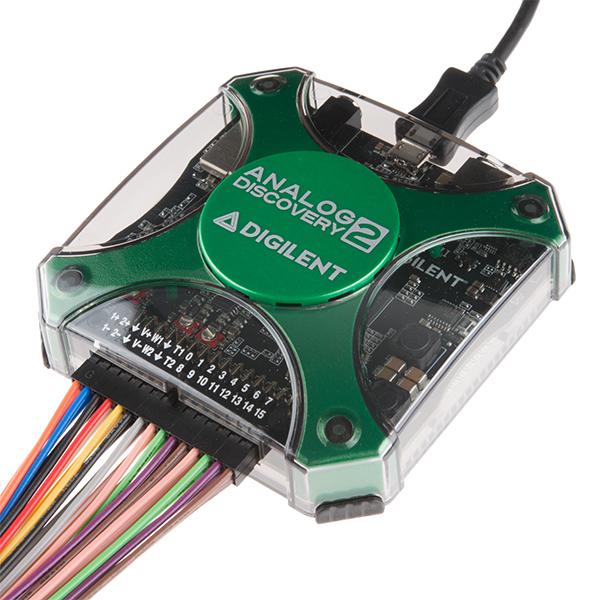
\includegraphics[width=0.4\textwidth]{AD2.jpg}
    \caption{Fotogafía del hardware del instrumento multifuncional Digilent Analog Discovery 2 (AD2). Este dispositivo cuenta con generador de señales arbitrarias, fuente regulada y osciloscopio, entre otros.}
    \label{fig:AD2}
\end{figure}

\begin{figure}[H]
    \centering
    \includegraphics[width=1\textwidth]{WF_WINDOW.png}
    \caption{Panel instrumental de WaveForms para el control y adquisición del AD2, donde se identifica la ventana de osciloscopio en la parte superior, el generador de señales en la parte inferior izquierda y la fuente de alimentación en la parte inferior derecha}
    \label{fig:wf_setup}
\end{figure}

\noindent Como plataforma de digitalización, se hace uso de la tarjeta ICTP-INFN ADC500, en adelante referida como ADC500 (fig \ref{fig:adc500}). Esta tarjeta está basada en un chip Texas Instruments ADC08500 \cite{ti_adc08500} monocanal de alta velocidad, con una frecuencia de muestreo de hasta 500 MHz, 8 bits de resolución y capacidad de digitalización de señales de hasta 1.2 V. Cumple con las especificaciones ANSI/VITA 57.1 y está equipada con un conector de tarjeta mezzanine FPGA (FMC) de bajo número de pines (LPC) \cite{crespo2021remote}.\\

\begin{figure}[H]
    \centering
    \includegraphics[width=0.8\textwidth]{ADC500.png}
    \caption{Plataforma de digitalización de señales ICTP-INFN ADC500. Se identifican sus principales partes: chip TI08500, conector FMC, conector SMA y pines de alimentación. Modificado de \cite{ictp_smr3765}.}
    \label{fig:adc500}
\end{figure}

\noindent
Para garantizar el correcto funcionamiento de la tarjeta, es necesario suministrarle 5 V y 1200 mA. La fuente de alimentación utilizada para este fin es la integrada en el AD2, que se conecta a una fuente auxiliar, ya que el puerto USB solo admite 500 mA. La conexión se ilustra en la figura \ref{fig:adc500_ad2}.

\begin{figure}[H]
    \centering
    \includegraphics[width=0.4\textwidth]{pines_adc500_ad2.png}
    \caption{Conexión entre ADC500 y Analog Discovery. Se describen los pines de alimentación de 5 V y GND, así como los puertos de entrada de señal del ADC500, que comprenden un conector SMA conectado en paralelo a un pin de conexión rápida.}
    \label{fig:adc500_ad2}
\end{figure}

\noindent Dado que la tarjeta ADC500 está diseñada para integrarse con un sistema de procesamiento basado en FPGA, se implementa un controlador de hardware descrito en lenguaje HDL, que mapea las conexiones para gestionar las funciones del chip. Estas funciones incluyen varios modos de calibración y rangos de digitalización \cite{ti_adc08500}. El controlador para el ADC500, desarrollado por el ICTP-MLAB, se utiliza atribuyendo la autoría correspondiente según su licencia \cite{ADC500driver}. En la figura \ref{fig:adc500driver} se observa la representación en diagrama de bloques del software AMD Xilinx Vivado \cite{vivado} del controlador mencionado.

\begin{figure}[H]
    \centering
    \includegraphics[width=0.4\textwidth]{ADC500_driver.png}
    \caption{Representación en diagrama de bloques del controlador del ADC500 diseñado en VHDL \cite{ADC500driver}.}
    \label{fig:adc500driver}
\end{figure}
% \noindent Según el fabricante, el ADC cuenta con un demultiplexor 1:2 que alimenta dos buses de salida LVDS (Low-Voltage Differential Signaling). Los datos de estos buses se entregan a una tasa de palabras de salida en cada bus equivalente a la mitad de la tasa de muestreo del ADC, y deben ser intercalados por el usuario para proporcionar palabras de salida a la tasa de conversión completa.  [6].

%\subsection{Montaje experimental: Digital processing platform based on FPGA SoC}

\noindent Teniendo en cuenta lo expuesto en la sección \ref{sec:digital_processing} y las características de alto rendimiento del ADC500 como sistema de digitalización, se utiliza una plataforma de procesamiento digital con capacidad de paralelización de procesos, alta disponibilidad de recursos de computación, reconfigurabilidad y flexibilidad. En este caso se trata de la tarjeta de desarrollo Avnet Digilent Zedboard (figura \ref{fig:zedboard}) \cite{avnet_zedboard}, basada en el SoC (System on Chip) Xilinx Zynq-7000 \cite{amd_zynq_7000}, que integra una FPGA Artix-7 y un procesador ARM Cortex-A9. Esta plataforma ofrece una amplia gama de periféricos tanto de propósito general como específico, incluyendo pines GPIO, pulsadores, interruptores, conectores de audio, interfaces de video HDMI y VGA, Ethernet, puertos USB, y, de particular relevancia para este trabajo, un conector FMC. Además, la Zedboard cuenta con interfaces de comunicación serial y JTAG para la configuración y programación del SoC FPGA.\\

\begin{figure}[H]
    \centering
    \includegraphics[width=1.0\textwidth]{zedboard_and_block.png}
    \caption{Fotogafía de la tarjeta de desarrollo FPGA SoC Avnet Digilent Zedboard y descripción en diagrama de bloques de la distribución de los periféricos en el PS y PL \cite{avnet_zedboard}.}
    \label{fig:zedboard}
\end{figure}

\noindent Para programar y configurar la plataforma FPGA SoC Xilinx Zynq-7000, se emplea el entorno de desarrollo unificado AMD Vitis \cite{vitis_xilinx}. Este entorno abarca tanto Vivado \cite{vivado} para el diseño y configuración de la FPGA (PL), como Vitis SDK para la programación del procesador embebido (PS). En este trabajo, el software Vivado se utiliza para configurar el hardware de control del ADC, los filtros para el procesamiento de señales y la gestión de la comunicación de alta velocidad. Este software permite visualizar scripts de descripción de hardware en bloques con entradas y salidas, permitiendo una abstracción modular de la lógica implementada.\\

% \noindent El flujo general de diseño para configurar la plataforma consta de dos etapas principales:
% \begin{enumerate}
%     \item Diseño y Configuración en Vivado:
%     \begin{itemize}
%         \item Cargar la configuración del mapeo de pines y puertos de la tarjeta de desarrollo (en este caso, la Zedboard).
%         \item Desarrollar el diseño del sistema digital en un lenguaje de descripción de hardware (HDL) como VHDL.
%         \item Generar el archivo bitstream, que contiene toda la información necesaria para configurar la lógica en la FPGA.
%     \end{itemize}
%     \item Programación en Vitis:
%     \begin{itemize}
%         \item Cargar el archivo bitstream generado en Vivado como plataforma de hardware en Vitis.
%         \item Programar el firmware del procesador embebido en un lenguaje de alto nivel (C o C++).
%         \item Finalmente, cargar la configuración de la FPGA y el firmware del procesador en el hardware, permitiendo que el sistema integral ejecute las acciones previstas.
%     \end{itemize}
% \end{enumerate}

% \noindent De acuerdo con los requisitos de la aplicación, las entradas y salidas del sistema en el PL, se asocian a componentes de memoria, como registros, FIFOs o RAM, accesibles desde el procesador (PS) mediante protocolos de interconexión entre el PL y el PS (véase la figura \ref{fig:fpga_soc}). Desde el entorno de programación de alto nivel del procesador, en este caso Vitis SDK, es posible interactuar con el hardware sintetizado en la FPGA para configurar parámetros del sistema a través de métodos de escritura y adquirir datos desde la memoria mediante métodos de lectura. No obstante, las herramientas proporcionadas por el fabricante, como los controladores del bus del PS, pueden resultar complejas de implementar para algunos usuarios debido a la cantidad de parámetros y el nivel de experticia requerido \cite{melo2019study}.

\noindent Para interconectar el PL y el PS, se utiliza el ComBlock \cite{core_comblock} (fig. \ref{fig:comblock_ictp}), un IP portable y altamente configurable diseñado para acceder a interfaces como registros, RAM y FIFOs, evitando la complejidad del bus del Sistema del Procesador (PS), que en el caso del Zynq-7000 es el bus de interconexión AXI y el AXI DMA como control de memoria \cite{axi_xilinx}.\\

% Este bloque de comunicaciones cuenta con:
% \begin{itemize}
% \item Hasta 16 registros de entrada y/o salida, configurables de 1 a 32 bits.
% \item Una memoria RAM de doble puerto, que ofrece una interfaz Simple RAM. La inclusión, el ancho de datos, el ancho de la dirección y la profundidad de la memoria son configurables.
% \item Dos FIFOs asincrónicos, uno de PL a PS y otro de PS a PL, con indicaciones de vacío/lleno, casi vacío/lleno y condiciones de subdesbordamiento/desbordamiento. La inclusión individual, el ancho de datos y la profundidad de la memoria son configurables.
% \end{itemize}

% \noindent En términos simples, el ComBlock actúa como una capa de abstracción para los buses AXI. En la versión del paquete IP de Vivado, se utiliza una interfaz AXI Lite para manejar los registros y FIFOs, mientras que la RAM se gestiona mediante una interfaz AXI Full como se ilustra en la figura \ref{fig:comblock_ictp}. 

\begin{figure}[H]
    \centering
    \includegraphics[width=0.8\textwidth]{comblock_ictp.png}
    \caption{Ilustración de la arquitectura de Comblock. En este se observa la utilidad del ComBlock como intermediador entre el PL y los buses AXI que interconectan con el PS. Adicionalmente se observan las interfaces de acceso a memoria que este bloque ofrece como registros, FIFO y RAM. Tomado de \cite{core_comblock}}
    \label{fig:comblock_ictp}
\end{figure}

% \noindent Sin embargo, este proceso es completamente transparente para el usuario, quien no necesita lidiar con las complejas configuraciones de estos buses. Como se ilustra en la figura \ref{fig:bd_comblock}, el ComBlock IP ha sido diseñado de manera modular, lo que permite su incorporación directa en los diagramas de bloques de hardware digital en Vivado como un componente adicional. Esto facilita la interconexión entre el PS, el diseño específico en el PL, y los componentes de memoria, todo de forma intuitiva para el usuario.

% \begin{figure}[h]
%     \centering
%     \includegraphics[width=0.8\textwidth]{bd.png}
%     \caption{Diagrama de bloques de un diseño real en Vivado donde se identifican los módulos del PS, el diseño específico de PL y la intercomunicación mediante Comblock}
%     \label{fig:bd_comblock}
% \end{figure}

% \noindent Con un diseño de hardware digital configurado en el PL, una interfaz de intercomunicación con el PS y acceso a memoria mediante Comblock, es posible concentrarse en la programación del PS para gestionar las funciones del slow control del DAQ. Esta programación se realiza en Vitis SDK, un entorno de desarrollo integrado (IDE) basado en Eclipse \cite{eclipse}, donde se desarrollan los scripts de firmware que controlan las funciones y periféricos del procesador. Además, el proyecto Comblock incluye un controlador en C que puede ser implementado en proyectos Baremetal o basados en FreeRTOS \cite{freertos}, todo ello desde el mismo entorno Vitis SDK. \\

% \noindent Aprovechando la estructura modular del diseño implementado en el PL, se procede inicialmente a describir cada módulo por separado, detallando la lógica configurada y sus respectivas funciones. Posteriormente, se abordará el diseño en su conjunto, analizando las interconexiones entre los módulos y destacando las diferentes configuraciones posibles. Esto permitirá demostrar la flexibilidad y versatilidad de esta metodología para el desarrollo de sistemas de adquisición y procesamiento de señales.\\

% \noindent Durante la fase de pruebas de los módulos de procesamiento digital de señales, es crucial poder visualizar las señales de salida generadas por estos módulos. Para lograrlo, se utiliza un módulo multiplexor (ver figura \ref{fig:bd_abstraction}), que permite seleccionar, desde un registro de salida del ComBlock, la señal que se almacenará en la FIFO y que, a su vez, se mostrará en la interfaz de Python. Esta metodología presenta varias ventajas importantes, como la capacidad de verificar el funcionamiento de cada módulo de procesamiento de señales de forma individual, sin necesidad de modificar el diseño del PL ni realizar una nueva síntesis cada vez que sea necesario corregir o mejorar la lógica del hardware.\\
\noindent Dado que el acceso a la información procesada por el PL se realiza a través del ComBlock, los módulos y filtros implementados en el PL, que se describen a continuación, se conectan de forma bidireccional al ComBlock durante la integración del sistema. Los registros de escritura del ComBlock se emplean para controlar el estado de los registros de entrada y control de los distintos módulos, mientras que las salidas de señal se envían a los elementos de lectura. Estos pueden ser registros para adquirir valores estáticos o FIFO y RAM para señales continuas, como las generadas por los filtros. Tanto los registros de lectura como escritura se configuran con un tamaño de 32 bits para permitir el manejo de valores de alto orden de magnitud. Por otro lado, la FIFO se configura con una profundidad de 4096 datos, valor comparable al manejado por los osciloscopios comerciales.\\

\noindent Teniendo en cuenta que la aplicación de este trabajo se centra en la adquisición y procesamiento de señales de sensores o detectores para extraer medidas de interés en procesos físicos, es fundamental contar con un sistema de visualización que permita inspeccionar las características de estas señales de forma similar a un osciloscopio (véase fig. \ref{fig:trigger_bd}). Este módulo, implementado en VHDL, compara la señal de salida del ADC500 con un umbral configurado por el usuario. Cuando la señal supera dicho umbral, se activa una señal tipo bandera, la cual habilita el registro de escritura de la FIFO del ComBlock, permitiendo el almacenamiento de datos a partir de la muestra en que se cumple la condición.

\begin{figure}[H]
    \centering
    \includegraphics[width=0.4\textwidth]{trigger_bd.png}
    \caption{Diagrama de bloques de Vivado de un módulo de trigger simple escrito en VHDL. Entre sus señales de entrada se observan el reloj del sistema, señal de reset, nivel del umbral de amplitud de la señal y señal digitalizada. A su salida se observa la señal para activar la escritura de la FIFO del ComBlock.}
    \label{fig:trigger_bd}
\end{figure}

% \noindent Tanto la señal de reloj (clk) como la de reinicio (reset) están conectadas al gestor de reloj y al sistema de reset, respectivamente. La señal de control del nivel de umbral, por su parte, está vinculada a un registro de salida del ComBlock, el cual puede ser configurado por el usuario a través de la interfaz UDMA en Python. De igual manera, desde esta interfaz es posible habilitar la lectura de la FIFO y extraer los datos almacenados una vez que el módulo de trigger ha activado la escritura en la FIFO. Finalmente, los datos de la señal, a partir del punto en que se cumple la condición de superación del umbral, pueden ser representados gráficamente utilizando un entorno especializado como matplotlib.\\

\noindent Sin embargo, esta lógica presenta una limitación al adquirir señales pulsadas, ya que solo se registra en la memoria la parte del pulso posterior al cruce del umbral. Esto impide la visualización completa de la forma del pulso, lo cual es problemático en aplicaciones como la detección de partículas, donde la forma completa del pulso es un parámetro de interés crucial. Para mitigar este inconveniente, se implementa la lógica de "pre-trigger time". Este sistema acumula muestras digitalizadas en un búfer y, una vez que se cumple la condición de disparo, tanto la porción posterior del pulso como una sección anterior, previamente almacenada, son concatenadas y enviadas a la memoria, permitiendo así la visualización integral del pulso. La lógica se estructura en tres etapas: la lógica de disparo, el temporizador de trigger y un búfer FIFO circular.\\


\noindent El primer módulo en VHDL (fig. \ref{fig:trigger_bd2}) implementa una lógica de disparo basada en cruce de nivel de amplitud, que detecta cuando una señal de entrada (\texttt{dataIn}) cruza un umbral (\texttt{threshold}) predefinido. La lógica permite seleccionar entre activación por cruce ascendente o descendente, controlado por el valor de \texttt{edge\_Select}. Si \texttt{edge\_Select} está en 0, el disparo se produce cuando \texttt{dataIn} pasa de un valor inferior al umbral a uno igual o superior. Si \texttt{edge\_Select} está en 1, el disparo ocurre cuando \texttt{dataIn} pasa de un valor superior al umbral a uno igual o menor. Este módulo está diseñado para procesar señales con un bus de datos configurable mediante el parámetro genérico \texttt{DATA\_BUS\_WIDTH}, sincronizándose con el reloj (\texttt{clk}) y una señal de reinicio asíncrono (\texttt{aresetn}).

\begin{figure}[H]
    \centering
    \includegraphics[width=0.4\textwidth]{trigger_bd2.png}
    \caption{Diagrama de bloques de Vivado del módulo de trigger.}
    \label{fig:trigger_bd2}
\end{figure}

\noindent El módulo de temporizador de la señal de disparo en VHDL (fig. \ref{fig:trigger_timer}) genera una señal de disparo (\texttt{trig\_out}) que se mantiene activa durante un tiempo determinado tras la detección de un evento en la entrada (\texttt{trig\_in}). La longitud del pulso de salida está controlada por la señal \texttt{pulse\_len}, que especifica el número de ciclos de reloj durante los cuales el disparo estará activo. Al detectar un flanco ascendente en \texttt{trig\_in}, se inicia un contador que incrementa en cada ciclo de reloj. Mientras el contador sea menor al valor de \texttt{pulse\_len}, la señal de disparo permanece en 1. Una vez que el contador alcanza este valor, se reinicia y \texttt{trig\_out} vuelve a 0.

\begin{figure}[H]
    \centering
    \includegraphics[width=0.4\textwidth]{trigger_timer.png}
    \caption{Diagrama de bloques de Vivado del módulo de timer del trigger.}
    \label{fig:trigger_timer}
\end{figure}

\noindent Finalmente, el código que describe un módulo VHDL llamado \texttt{circular\_FIFO} (figura \ref{fig:fifo_circular}), implementa un buffer circular, utilizado comúnmente para almacenar y gestionar datos de manera eficiente. Este módulo tiene dos puertos: uno para escritura y otro para lectura, controlados mediante las señales \texttt{wr\_en} (habilitación de escritura) y \texttt{rd\_en} (habilitación de lectura). El tamaño del buffer está determinado por los parámetros genéricos \texttt{RAM\_WIDTH} y \texttt{RAM\_DEPTH}, que definen el ancho y la profundidad de la memoria.\\

\noindent El módulo utiliza dos punteros: \texttt{head}, que indica la posición de escritura, y \texttt{tail}, que indica la posición de lectura. Cuando se escribe un dato (siempre que el buffer no esté lleno), el puntero \texttt{head} se incrementa y el dato se almacena en la posición correspondiente de la memoria (\texttt{ram}). De manera similar, cuando se habilita la lectura y el buffer no está vacío, el puntero \texttt{tail} se incrementa y el dato leído se extrae de la memoria. Las señales \texttt{empty\_i} y \texttt{full\_i} indican si el buffer está vacío o lleno, respectivamente, y se basan en el valor de un contador (\texttt{fill\_count\_i}) que rastrea cuántos elementos hay almacenados en el buffer.\\

\noindent El procedimiento \texttt{incr} garantiza que los punteros de lectura y escritura se envuelvan correctamente cuando alcanzan el final del buffer, reiniciándose a la primera posición para mantener el comportamiento circular. La arquitectura incluye procesos para actualizar los punteros y manejar la escritura/lectura en la memoria del buffer, así como para gestionar el conteo de elementos almacenados.

\begin{figure}[H]
    \centering
    \includegraphics[width=0.4\textwidth]{ring_buffer.png}
    \caption{Diagrama de bloques de Vivado del módulo de FIFO circular.}
    \label{fig:fifo_circular}
\end{figure}

\noindent La interconexión entre los tres módulos está organizada de la siguiente manera: la salida del módulo de disparo (trigger) alimenta la entrada del temporizador (timer), y la salida del temporizador activa la escritura en el FIFO circular. Además, el FIFO circular debe incluir un módulo de lógica de registro de desplazamiento (shift register) para configurar el número de muestras a adquirir antes de que se produzca el disparo.\\

\noindent Para visualizar una señal con mayor detalle o, por el contrario, abarcar una ventana de tiempo más amplia, es necesario implementar una etapa de control temporal en la tasa de muestreo. Con este propósito, se diseña un módulo de decimación (fig. \ref{fig:decimator_bd}), el cual actúa como un divisor de la frecuencia de muestreo. Este módulo recibe como entradas la señal de reloj y reset, los datos provenientes del ADC, y el valor de división (N). Este último está conectado a un registro de escritura del comblock, que el usuario puede configurar desde la interfaz de Python. Para garantizar un escalamiento coherente con la decimación aplicada, es fundamental ajustar el eje temporal de la gráfica de visualización de las señales en la interfaz de Python utilizando la relación

\begin{equation}
    \frac{N_{\text{data}}*d}{f_{\text{ADC}}}
\end{equation}

\noindent donde $N_{\text{data}}$ es el número de datos leídos de la FIFO, $d$ es el factor de decimación y $f_{\text{ADC}}$ es la frecuencia de muestreo del ADC.\\

\begin{figure}[h]
    \centering
    \includegraphics[width=0.4\textwidth]{decimator_bd.png}
    \caption{Diagrama de bloques de Vivado de un módulo de decimación escrito en VHDL.}
    \label{fig:decimator_bd}
\end{figure}

\noindent El procesamiento de señales implementado incluye un módulo de media móvil de ventana fija en VHDL (fig.  \ref{fig:MA_bd}), que se utiliza para suavizar señales mediante el filtrado de las mismas. Este filtro realiza un promedio de los valores de una ventana deslizante sobre la señal de entrada, lo que ayuda a reducir el ruido de alta frecuencia y a estabilizar la señal. El filtro está diseñado para procesar datos de entrada en un formato de vector de bits (\texttt{i\_data}) y generar una señal de salida suavizada (\texttt{o\_data}). El tamaño de la ventana de promedio se define mediante el parámetro genérico \texttt{G\_AVG\_LEN\_LOG}, que determina el número de muestras a considerar en cada cálculo de promedio. El módulo mantiene un acumulador (\texttt{r\_acc}) que suma los valores de las muestras actuales y un arreglo (\texttt{p\_moving\_average}) que almacena las muestras de la ventana actual. Con cada nuevo dato de entrada, el filtro desplaza la ventana y actualiza el promedio. La señal de salida (\texttt{o\_data}) se calcula dividiendo el valor acumulado entre el número de muestras en la ventana, logrando así la suavización de la señal. Este enfoque ayuda a eliminar las fluctuaciones rápidas y el ruido de alta frecuencia, proporcionando una representación más estable de la señal. Esto permite analizar directamente su componente de baja frecuencia o ingresarla a un filtro posterior que requiera una señal con bajo nivel de ruido electrónico, como es el caso del shaper trapezoidal.

\begin{figure}[h]
    \centering
    \includegraphics[width=0.4\textwidth]{moving_average_bd.png}
    \caption{Diagrama de bloques de Vivado de un módulo de media móvil simple escrito en VHDL. Entre sus señales de entrada se observan el reloj del sistema, señal de reset, señal de habilitación y señal digitalizada. A su salida se observa la señal filtrada.}
    \label{fig:MA_bd}
\end{figure}

\noindent El diseño del filtro trapezoidal comienza con la simulación de los pulsos provenientes de un detector genérico. Se consideran una serie de parámetros clave, como la carga del detector (\( Q \)), la capacitancia (\( C_f \)), la constante de tiempo (\( \tau \)) y el período de muestreo (\( T_s \)). La constante de tiempo \( \tau \) se define como el inverso de la frecuencia del sistema, lo que determina la velocidad de decaimiento exponencial de la señal. Asimismo, el período de muestreo genera un número de muestras por segundo igual a \( N = 1/T_s \). El término \( d \), calculado como \( \exp(-T_s/\tau) \), representa el factor de decaimiento exponencial entre muestras consecutivas. La señal de prueba se genera en un rango de tiempo arbitrario, con un retardo inicial para simular las condiciones reales de detección.\\

\noindent El filtro se basa en una ventana deslizante que realiza una serie de operaciones (fig. \ref{fig:trapez_meth}) sobre las muestras de la señal de entrada, acumulando los resultados en la salida final del filtro. Los tiempos de subida (\( t_a \)) y bajada (\( t_b \)) definen el comportamiento del filtro, controlando el alisado y la duración del pulso trapezoidal. El algoritmo calcula la salida del filtro trapezoidal utilizando las diferencias entre las muestras de la señal en distintos puntos temporales, ajustadas por el factor de decaimiento \( d \). Esta operación tiene en cuenta los puntos correspondientes a los tiempos \( t_a \), \( t_b \), y un retardo adicional, sumando las contribuciones correspondientes y normalizándolas según el tiempo de subida. Además, la función incorpora términos de corrección para evitar inestabilidades numéricas, asegurando un rendimiento óptimo del filtro en condiciones de detección de señales.

\begin{figure}[H]
    \centering
    \includegraphics[width=1.2\textwidth]{trap_methodology.png}
    \caption{Ecuaciónes de recurrencia y diagrama de funciones del filtro trapezoidal implementado.}
    \label{fig:trapez_meth}
\end{figure}

\noindent El filtro FIR se aplica a través de la convolución de la señal sintética con los pesos \( K \), \( L \) y \( M \) que rigen su comportamiento. Al modificar estos parámetros, se obtienen diferentes respuestas del filtro, optimizándolas según la aplicación. En este caso, se busca que el filtro convierta pulsos exponenciales en pulsos de altura proporcional para facilitar la extracción de su amplitud y, posteriormente, de la energía depositada. También se pretende que realice *pile-up rejection*, permitiendo diferenciar eventos individuales al ubicar los pulsos trapezoidales sobre la misma línea base. Todo esto con el objetivo de enviar los pulsos trapezoidales al discriminador de eventos y, posteriormente, al MCA para la generación de histogramas de amplitud.\\

\noindent Los parámetros de forma del filtro, K, L y M, se calculan en Python de manera offline a partir de una señal real generada con el AD2 utilizando previamente la señal sintetizada en Python a la que se le añade una componente de ruido, mejorando así la simulación de una señal de detector real. Posteriormente, esta señal se adquiere con el DAQ y se procesa mediante un filtro de media móvil, lo que permite reducir el ruido de alta frecuencia. Considerando la frecuencia de muestreo del ADC500 y el factor de decimación, se utilizan ecuaciones recursivas implementadas en Python para graficar el efecto del filtro sobre la señal, ajustando los parámetros hasta lograr un resultado óptimo.\\ 

\noindent Posteriormente, se implementa el filtro FIR trapezoidal en VHDL (fig. \ref{fig:trapez_bd}), basado en las ecuaciones de recurrencia descritas y en los parámetros K, L y M optimizados. Este filtro recibe las muestras digitalizadas, previamente filtradas de alta frecuencia mediante una media móvil, y acumula valores según las posiciones de las muestras dentro de un buffer. A través de las operaciones definidas entre las muestras y los parámetros K, L y M, se establecen límites y pesos que controlan aspectos fundamentales del filtro, tales como el tiempo de subida, el flat top y el tiempo de bajada.

\begin{figure}[h]
    \centering
    \includegraphics[width=0.4\textwidth]{trapez.png}
    \caption{Diagrama de bloques de Vivado del filtro trapezoidal.}
    \label{fig:trapez_bd}
\end{figure}

\noindent Por otro lado, se implementa un Analizador Multicanal (MCA) embebido en el PL, aprovechando las capacidades avanzadas de la memoria True Dual Port RAM a través del ComBlock. Este módulo permite gestionar de manera eficiente y rápida los pulsos provenientes de detectores de radiación, facilitando la construcción de histogramas precisos de las amplitudes de los pulsos. Si el detector utilizado produce pulsos cuya altura es proporcional a la energía depositada por la partícula detectada, estos histogramas pueden ser empleados para generar espectros de distintos tipos, tras una calibración adecuada, según la técnica experimental utilizada, como Raman o Mössbauer, por ejemplo.\\

\noindent El MCA consta de dos módulos: el sistema de discriminación de altura de pulsos pulsos y el gestor de memoria RAM. El submódulo discriminador de pulsos \ref{fig:disc_bd} es un sistema que compara la amplitud de un pulso con un rango de valores determinado por dos umbrales: un umbral inferior y un umbral superior, ambos específicos para cada canal. Estos umbrales están definidos en función de la profundidad y el ancho de la memoria, lo que establece la resolución del sistema. Para que un pulso sea detectado, su amplitud debe estar entre el umbral inferior y el umbral superior asignados a una dirección específica de la memoria RAM. Cuando un pulso se encuentra dentro de este rango, se incrementa en uno el valor del contador almacenado en la dirección de memoria correspondiente. Este submódulo transmite la información al módulo gestor de RAM, indicando qué dirección de memoria debe actualizarse para reflejar el incremento en el contador, según el umbral superado.\\

\begin{figure}[H]
    \centering
    \includegraphics[width=0.4\textwidth]{disc_bd.png}
    \caption{Diagrama de bloques de Vivado del submódulo discriminador de pulsos del MCA.}
    \label{fig:disc_bd}
\end{figure}

\noindent El módulo de VHDL \texttt{bram\_incr} (fig. \ref{fig:mca_bd}) implementa una máquina de estados que gestiona operaciones en un bloque de memoria RAM (BRAM). Su funcionalidad principal es leer un valor de una dirección específica del BRAM, incrementar ese valor en uno, y luego almacenar el resultado de vuelta en el BRAM. El módulo recibe señales de entrada para la dirección del BRAM y la disponibilidad de datos, y utiliza una máquina de estados con cuatro etapas para controlar el flujo de operaciones. Las señales internas controlan la lectura, el incremento y la escritura de datos en el BRAM.\\

\begin{figure}[H]
    \centering
    \includegraphics[width=0.4\textwidth]{mca.png}
    \caption{Diagrama de bloques de Vivado del gestor de RAM del MCA.}
    \label{fig:mca_bd}
\end{figure}

\noindent Como se mencionó anteriormente, los módulos de PL procesan las señales del ADC, enviándolas al ComBlock para su adquisición por el PS y posterior transmisión al usuario. La estructura general del diseño de bloques sigue la topología mostrada en la figura \ref{fig:bd}. En el recuadro del lado derecho (PL), se encuentran el controlador del ADC500, los diferentes filtros y el ComBlock, mientras que en el lado izquierdo se ubica el controlador del PS.

\begin{figure}[H]
    \centering
    \includegraphics[width=1\textwidth]{bd.png}
    \caption{Diagrama de bloques de Vivado donde se observa la interconexión típica entre PL y PS mediada por el ComBlock.}
    \label{fig:bd}
\end{figure}

\noindent Para la implementación de la interfaz de comunicación bidireccional entre el usuario y el sistema de procesamiento (PS), se emplea el UDMA (Universal Direct Memory Access), un sistema desarrollado en el laboratorio multidisciplinario del ICTP (MLAB) como un conjunto de herramientas de control diseñado para conectar una PC con la lógica personalizada en un SoC-FPGA \cite{crespo2021remote}. El UDMA actúa como un puente entre un generador y un receptor de datos basado en un sistema operativo de tiempo real (RTOS), permitiendo realizar operaciones de lectura y escritura en cualquier memoria dentro del PS por medio del protocolo TCP/IP a través del puerto de Ethernet. Está compuesto por una librería en C y otra en Python, que, al trabajar en conjunto, proporcionan una plataforma de control accesible para el hardware y software integrados en el SoC-FPGA. En particular, el UDMA puede implementarse junto con el ComBlock para permitir al usuario acceder a la información que entra y sale del PL mediante una interfaz de alto nivel basada en Python, proporcionando así el último eslabón de la cadena del DAQ, como se muestra en la figura \ref{fig:daq-ictp}.

\begin{figure}[H]
    \centering
    \includegraphics[width=1.0\textwidth]{daq_ictp.png}
    \caption{Diagrama esquemático del DAQ implementado en este trabajo, donde se observa el flujo de información desde un sistema físico hasta el usuario, particularizando el diagrama \ref{fig:DAQ_generic} con las etapas descritas en este trabajo como el ADC500, FPGA SoC Zynq7000 y UDMA.}
    \label{fig:daq-ictp}
\end{figure}

\noindent Desde la perspectiva del usuario (PC), se importa la librería UDMA en Python, la cual está basada en una clase que actúa como un envoltorio para un socket TCP y emplea un protocolo simple para gestionar los comandos. Al instanciar la clase, se especifican la dirección IP y el puerto del servidor, estableciendo el socket, lo que permite ejecutar comandos proporcionando los parámetros adecuados \cite{udma_gitlab}. En la figura \ref{fig:udma_python} se muestra un ejemplo del uso de la interfaz UDMA en Python, donde se observa la importación de la librería, la instanciación del objeto UDMA y el uso de métodos para la lectura y escritura de los elementos de memoria asignados en el ComBlock.

\begin{figure}[H]
    \centering
    \includegraphics[width=0.4\textwidth]{udma_python.png}
    \caption{Interfaz de usuario del DAQ implementado basada en Python. Se observa la importación, instanciación y uso del paquete UDMA, que permite la comunicación del usuario con el PS y por tanto con el PL a través del ComBlock.}
    \label{fig:udma_python}
\end{figure}

\noindent Cuando se ejecutan los comandos del UDMA, la librería de Python está diseñada para enviar al usuario una estructura de mensaje de confirmación ("acknowledge") que indica si hubo algún error en la ejecución. Si el comando es de escritura, la librería confirma los valores enviados; si es de lectura, proporciona los datos correspondientes a la adquisición. En el caso de la lectura de la memoria FIFO o RAM del ComBlock, los datos obtenidos, ya sea en forma de arreglo o como transmisión en tiempo real, pueden representarse gráficamente o en tablas utilizando librerías especializadas de Python, o procesarse de manera offline para su posterior análisis. En la figura \ref{fig:setup1} se muestra el hardware utilizado y su conexión.

\begin{figure}[H]
    \centering
    \includegraphics[width=0.7\textwidth]{SETUP1.png}
    \caption{Fotografía del hardware del DAQ implementado en este trabajo. A la derecha se observa el AD2 como instrumento generador de señales arbitrarias y fuente de alimentación para el ADC500, a continuación se aprecia la tarjeta ADC500 acoplada mediante el puerto FMC a la tarjeta de desarrollo del FPGA SoC Zynq7000 y las conexiones con el computador de escritorio para la interacción con el usuario.}
    \label{fig:setup1}
\end{figure}

\newpage

\section{Resultados}

\noindent Como se explicó anteriormente en la sección de Montaje experimental y metodología, la implementación efectiva del DAQ requiere la correcta conexión de los bloques de control, adquisición y procesamiento digital al ComBlock, así como la programación del UDMA en el PS como interfaz de comunicación y el desarrollo de una interfaz de usuario en Python (ver fig. \ref{fig:daq-ictp}). Por lo tanto, el primer resultado significativo de este trabajo es la integración de las etapas descritas y la obtención de datos que confirman implícitamente su correcto funcionamiento. Esto se evidencia, por ejemplo, en el encendido de los LEDs de la tarjeta ADC500 (fig. \ref{fig:ADC500_ON}) al enviar el comando  

\begin{verbatim}
    CTR_ADC_OUT_REG = 0
    INIT_ADC = 128
    oudma.write_reg(CTR_ADC_OUT_REG, INIT_ADC)
\end{verbatim}
 
\noindent desde la interfaz de Python, teniendo en cuenta que el valor 128 es una instrucción interna del ADC500 para su encendido y el puerto de control de encendido del bloque de Vivado del controlador del ADC500 \ref{fig:adc500driver} se encuentra conectado al registro de escritura 0 del ComBlock\\

\begin{figure}[H]
    \centering
    \includegraphics[width=0.5\textwidth]{adc500_on.jpg}
    \caption{Fotografía del ADC500 con los LEDs indicadores encendidos tras la ejecución del comando de encendido desde la interfaz de usuario en Python a través del UDMA.}
    \label{fig:ADC500_ON}
\end{figure}

\noindent Dado que la cadena de flujo de datos desde el ADC500 hasta la interfaz de usuario opera correctamente, se dirige el enfoque de las pruebas y sus resultados hacia los módulos de procesamiento de señales configurados en el PL o FPGA. Para ello, se emplean señales sintéticas que simulan la respuesta real de sensores o detectores, generadas por el AD2. Esto permite validar el funcionamiento de dichos módulos, variando parámetros de la señal como su forma, amplitud, offset, frecuencia y proporción de ruido añadido. En particular, se implementan señales sinusoidales, pulsos exponenciales y trenes de pulsos que presentan características similares a las señales típicamente generadas por sensores o detectores.\\

\noindent Inicialmente, se muestra el modo osciloscopio, donde se valida la capacidad de modificar la ventana temporal de adquisición desde la interfaz de usuario en Python, utilizando señales de prueba para comprobar que el período de la señal corresponde con el adquirido. A continuación, se describe el funcionamiento de los filtros configurados, como la media móvil y el "shaper" trapezoidal. Finalmente, se presenta el funcionamiento del MCA (Analizador Multicanal) o generador de histogramas multifuncional, utilizando un flujo continuo de pulsos de diferentes amplitudes como fuente, simulando la respuesta de un detector de radiación ante una fuente radiactiva o similares.\\

\noindent En la figura \ref{fig:parameters1}, se presenta la estructura característica de la interfaz de usuario en Python, donde se pueden observar los comandos de control utilizados para configurar los distintos módulos de hardware en la FPGA, mediante el método de escritura en registros del ComBlock a través de la instancia del UDMA. Asimismo, se muestra el comando para la lectura de la FIFO del ComBlock, y finalmente, la utilización de la herramienta gráfica \texttt{matplotlib} para la visualización de los datos obtenidos.

\begin{figure}[H]
    \centering
    \includegraphics[width=0.5\textwidth]{parameters1.png}
    \caption{Interfaz de usuario de Python donde se evidencia el uso de métodos de escritura y lectura de la librería UDMA para el control y adquisición a través del ComBlock.}
    \label{fig:parameters1}
\end{figure}

\noindent De especial importancia es el comando \texttt{oudma.write\_reg(MUX\_MODE, RAW\_ADC)}, ya que este permite seleccionar la señal que entra a la FIFO del ComBlock para su visualización al controlar un multiplexor instanciado en el hardware. Este multiplexor cuenta con los modos \texttt{RAW\_ADC} para observar la señal del ADC500 después del decimador, \texttt{MA\_FILTER} para observar la salida del filtro pasabajos de media móvil y \texttt{SHAPER} para observar la salida del filtro trapezoidal. Debe darse por sentado que, para la obtención de cada resultado, se ejecuta el comando que selecciona la salida de cada filtro.\\

\noindent Para probar el módulo de decimación, que permite controlar la ventana temporal de adquisición, se configura una señal periódica sinusoidal sin ruido añadido, ya que esto facilita la comprobación de cómo se modifica la ventana temporal. En este caso, la señal tiene un período de 50 $\mu$s y una amplitud de 50 mV.

\begin{figure}[H]
    \centering
    \includegraphics[width=0.5\textwidth]{wf1.png}
    \caption{Señal sinusoidal con $T = 50 \mu s$ generada con el AD.}
    \label{fig:signal1AD}
\end{figure}

\noindent En la figura se muestra el resultado de la adquisición de la señal anterior con valores de decimación de 50 y 10 y umbral de trigger configurado en 1500. En ambas gráficas se observa que la señal corresponde a una sinusoidal con un período de 50 $\mu$s que inicia en el valor de amplitud de 1500, validando el funcionamiento de la lógica de trigger simple. Sin embargo, en la primera gráfica, un valor de decimación más alto genera una ventana temporal de adquisición mayor, lo que permite observar varios períodos de la señal. En contraste, en la segunda gráfica, se observa solo un período de la señal, pero con mayor nivel de detalle. 

\begin{figure}[H]
    \centering
    \includegraphics[width=1\textwidth]{result_osc_seno1.png}
    \caption{Señal adquiAdquisición de una señal sinusoidal con un período de 50 $\mu$s y una amplitud de 50 mV. A la izquierda se observa la señal adquirida con un valor de decimación de 50, donde se capturan varios períodos completos. A la derecha, se muestra la señal con un valor de decimación de 10, permitiendo una mayor resolución temporal en un único período.}
    \label{fig:signal1DAQ}
\end{figure}

\noindent Para validar la capacidad del sistema en la adquisición de señales pulsadas, típicas en la detección de partículas y radiación, se generó con el AD2 una señal de pulsos exponenciales. A esta señal, con una frecuencia de 20 kHz, se le añadió un 10\% de ruido sobre su amplitud, simulando así condiciones realistas de medición en entornos experimentales.

\begin{figure}[H]
    \centering
    \includegraphics[width=0.5\textwidth]{wf2.1.png}
    \caption{Señal pulsada de tipo exponencial decreciente con ruido añadido de 10\% generada con el AD2.}
    \label{fig:signal2.1DAQ}
\end{figure}

\noindent En la figura \ref{fig:signalexpDAQ} se observa la adquisición de la señal pulsada utilizando el DAQ implementado. De manera similar al caso de la señal sinusoidal, se verifica que el decimador controla eficazmente la ventana temporal de adquisición al ajustar la tasa de muestreo del sistema. En la gráfica de la izquierda, un valor de decimación mayor permite visualizar un mayor número de pulsos, mientras que en la gráfica de la derecha, un valor de decimación menor permite apreciar con mayor detalle la forma de la señal.

\begin{figure}[H]
    \centering
    \includegraphics[width=1\textwidth]{result_exp_1.png}
    \caption{Señal pulsada exponencial adquirida utilizando el sistema DAQ implementado, con valores de decimación de 50 (izquierda) y 10 (derecha). En la gráfica de la izquierda se visualizan múltiples pulsos debido a la mayor ventana temporal de adquisición, mientras que en la derecha, con un valor de decimación menor, se observa con mayor detalle la forma de un solo pulso.}
    \label{fig:signalexpDAQ}
\end{figure}

A partir de parámetros típicos de pulsos provenientes de detectores de radiación, se genera un conjunto de datos en Python (ver fig. \ref{fig:pulses_pileup}) que simula un tren de pulsos exponenciales decrecientes. Estos pulsos presentan el fenómeno de pile-up, lo cual resulta útil para el ajuste de los filtros implementados y para la validación de ciertas funcionalidades del sistema de adquisición de datos (DAQ).

\begin{figure}[H]
    \centering
    \includegraphics[width=1\textwidth]{simul_pileup.png}
    \caption{Simulación de pulsos sintéticos en Python que representan la respuesta típica de un detector de radiación. Se aprecia el fenómeno de pile-up. esta señal se exporta como archivo de datos que puede utilizar el AD2 para generar una señal real con su forma.}
    \label{fig:pulses_pileup}
\end{figure}

\noindent El conjunto de datos es exportado a un archivo .CSV, el cual puede ser leído por el software AD2 WaveForms para generar una señal que modula sus características, como se observa en la parte izquierda de la figura \ref{fig:trenDAQ}. A su vez, en la parte derecha se muestra la gráfica de los datos adquiridos por el DAQ con el parámetro de decimación ajustado para observar una ventana temporal del orden de la imagen de la izquierda.

\begin{figure}[H]
    \centering
    \includegraphics[width=1\textwidth]{tren_pulsos_result.png}
    \caption{Señal tren pulsos exponencial adquirida}
    \label{fig:trenDAQ}
\end{figure}

\noindent  El diseño del filtro de media móvil comienza en Python, donde se exploran diferentes algoritmos basados en el filtro FIR descrito en la sección de procesamiento digital del marco teórico. Durante este análisis, se identifican variaciones en la eficiencia de los algoritmos en términos de procesamiento, tomando como métrica clave la capacidad para atenuar las componentes de alta frecuencia, como el ruido electrónico, utilizando la menor cantidad posible de muestras $N$. Se concluye que el algoritmo más eficiente es aquel que emplea un acumulador de muestras y realiza la división por un valor de $N$ que es potencia de 2. Esta elección proporciona una ventaja significativa, ya que simplifica las operaciones en el diseño posterior del filtro en VHDL.\\

\noindent En la figura \ref{fig:SMA}, se muestra la aplicación de este filtro, diseñado en Python, a una señal sinusoidal con un ruido añadido equivalente al 30\% de su amplitud, simulando la respuesta de un sensor en condiciones de alto ruido electrónico. Se observa claramente la recuperación de la señal original al eliminar de manera efectiva las componentes de alta frecuencia.

\begin{figure}[H]
    \centering
    \includegraphics[width=0.9\textwidth]{SMA.png}
    \caption{Resultado de diseño de media móvil implementado en Python para probar el concepto}
    \label{fig:SMA}

\end{figure}

\noindent Tras la configuración del filtro diseñado en VHDL en el PL, se genera con el AD2 una señal sinusoidal de 10 kHz con un ruido añadido equivalente al 20\% de la amplitud de la señal. Esta señal se ingresa al DAQ, y desde la interfaz de usuario en Python se selecciona el canal de media móvil en el multiplexor para observar el efecto del filtro sobre la señal real, como se muestra en la figura \ref{fig:signal1MADAQ}.

\begin{figure}[H]
    \centering
    \includegraphics[width=1\textwidth]{osc_MA1.png}
    \caption{A la izquierda se muestra la gráfica de la señal sinusoidal de 10 kHz con un 20\% de ruido añadido sin filtrar, mientras que a la derecha se observa la salida del filtro de media móvil. El efecto del filtro es evidente al reducir las componentes de alta frecuencia y mejorar la representación de la señal original.}
    \label{fig:signal1MADAQ}
\end{figure}

\noindent De manera similar, se realiza la prueba con una señal sinusoidal de 50 kHz, a la que se añade un 10\% de ruido en su amplitud. Se observa la salida del filtro de media móvil, evidenciando su capacidad para atenuar el ruido y recuperar la señal original.

\begin{figure}[H]
    \centering
    \includegraphics[width=1\textwidth]{osc_MA2.png}
    \caption{A la izquierda se muestra la gráfica de la señal sinusoidal de 50 kHz con un 10\% de ruido añadido, mientras que a la derecha se observa la salida del filtro de media móvil. El filtro atenúa eficazmente las componentes de alta frecuencia, permitiendo una mejor recuperación de la señal original.}
    \label{fig:signal2MADAQ}
\end{figure}

\noindent Se introduce en el filtro una señal de tipo pulso exponencial decreciente con un 10\% de ruido añadido a su amplitud, con el objetivo de evaluar la respuesta del filtro ante señales pulsadas, simulando condiciones reales de filtrado de señales provenientes de detectores. Como se observa en la figura \ref{fig:signal3MADAQ}, el filtro elimina de manera efectiva gran parte de las componentes de ruido electrónico, permitiendo revelar la forma del pulso y sus características físicas de interés.

\begin{figure}[H]
    \centering
    \includegraphics[width=1\textwidth]{osc_MA3.png}
    \caption{Señal pulsada exponencial con ruido filtrada por MA 10KHz con 10 porciento de ruido sumado}
    \label{fig:signal3MADAQ}
\end{figure}

\noindent Se repite el mismo procedimiento, aumentando la frecuencia a 100 kHz y la componente de ruido añadido al 20\%, con el fin de poner a prueba el sistema ante una mayor frecuencia y la difusión de la señal pulsada. Sin embargo, se observa que el filtro aún puede mejorar la relación señal-ruido, entregando pulsos que pueden ser utilizados en etapas posteriores.

\begin{figure}[H]
    \centering
    \includegraphics[width=1\textwidth]{exp100khz_ma.png}
    \caption{A la izquierda se muestra la gráfica de la señal pulsada de 100 kHz con un 20\% de ruido añadido, mientras que a la derecha se observa la salida del filtro de media móvil. A pesar de la mayor frecuencia y el aumento del ruido, el filtro mejora la relación señal-ruido, permitiendo que los pulsos sean adecuados para etapas posteriores.}
    \label{fig:signal4MADAQ}
\end{figure}

\noindent Haciendo uso de un tren de pulsos exponenciales que simulan un conjunto de eventos de un detector y presentan pile-up (fig. \ref{fig:trenDAQ}), se añade en WaveForms una componente de ruido del 10\% de su amplitud para observar el comportamiento del filtro de media móvil ante este tipo de señales. Se encuentra que, al igual que en los casos anteriores, el filtro tiene la capacidad de eliminar componentes de alta frecuencia, permitiendo apreciar mejor la forma y los detalles de la señal.

\begin{figure}[H]
    \centering
    \includegraphics[width=1\textwidth]{tren_ma.png}
    \caption{A la izquierda se muestra el tren de pulsos exponenciales simulado con pile-up y un 10\% de ruido añadido generados a 10kHz. A la derecha se observa la salida del filtro de media móvil. El filtro demuestra su capacidad para eliminar componentes de alta frecuencia, lo que permite una mejor visualización de la forma y los detalles de la señal.}
    \label{fig:trenMA}
\end{figure}

\noindent Como se expuso en la sección anterior, donde se desarrolla la metodología de diseño del filtro trapezoidal, inicialmente se aplica el filtro en Python para calcular los coeficientes \( K \), \( L \) y \( M \) que generan la mejor respuesta a la señal. El resultado inicial para un tren de pulsos sintetizados, que refleja las características de una señal generada por un detector, se observa en la figura \ref{fig:trap_pileup}.\\

\noindent Se puede apreciar el efecto que tiene el filtro shaper trapezoidal sobre los pulsos exponenciales. La primera observación es que el filtro genera un pulso trapezoidal, similar a un pulso cuadrado, proporcional a la altura del pulso respecto a la línea base. Además, se evidencia su capacidad para realizar *pile-up rejection*, ya que separa pulsos exponenciales adyacentes y los coloca sobre la línea base, revelando la amplitud real de cada uno.

\begin{figure}[H]
    \centering
    \includegraphics[width=1\textwidth]{trap_pileup.png}
    \caption{Aplicación del filtro trapezoidal diseñado en Python a los pulsos anteriores usando Python}
    \label{fig:trap_pileup}
\end{figure}

\noindent No obstante, para obtener los coeficientes adecuados que se configuran en el filtro que se instanciará en el PL para procesamiento continuo, es necesario realizar la calibración con la señal real. Por lo tanto, se ingresa al DAQ la señal de un tren de pulsos exponenciales con ruido, generada con el AD2, y se hace pasar por el filtro de media móvil para eliminar las componentes de alta frecuencia o ruido. Una vez adquirida esta señal con el UDMA en Python, se aplica la función del filtro trapezoidal creada anteriormente, variando los parámetros \( K \), \( L \) y \( M \) hasta observar una respuesta adecuada del shaper trapezoidal. En particular, se encuentran los valores \( K = 57 \), \( L = 5 \) y \( M = 100 \), con los cuales se observa una buena forma de los pulsos trapezoidales, un adecuado *pile-up rejection* y la ubicación de los pulsos sobre la misma línea base. En la figura \ref{fig:trap_design_python} se observan tres gráficas: en la primera, se muestra la señal adquirida por el DAQ después del módulo de decimación; en la segunda, se observa la salida del módulo de media móvil que se ingresa al módulo de shaper trapezoidal; y en la tercera, se presenta la respuesta del filtro trapezoidal en Python, optimizado con los parámetros mencionados.

\begin{figure}[H]
    \centering
    \includegraphics[width=1\textwidth]{filters_result.png}
    \caption{Se muestran tres gráficas relacionadas con el procesamiento de la señal. En la primera gráfica, se presenta la señal adquirida por el DAQ tras el módulo de decimación. La segunda gráfica muestra la salida del módulo de media móvil que se ingresa al módulo de shaper trapezoidal. Finalmente, la tercera gráfica representa la respuesta del filtro trapezoidal en Python, optimizado con los parámetros de forma $K=57, L=5, M=100$.}
    \label{fig:trap_design_python}
\end{figure}

\noindent Luego de la implementación del módulo de filtro shaper trapezoidal en VHDL, se configuran los parámetros optimizados de forma y se realiza la interconexión con el resto del sistema. A continuación, se lleva a cabo una prueba de funcionamiento utilizando la herramienta Vivado ILA (Integrated Logic Analyzer), conectando pruebas a la señal decimada de salida del ADC500, a la salida del módulo de media móvil y a la salida del filtro trapezoidal. Tras la síntesis del diseño, se obtienen los resultados mostrados en la figura \ref{fig:ILAtrap}, donde se observan las tres señales y se confirma el funcionamiento del filtro trapezoidal a nivel de la FPGA utilizando el ILA.\\

\noindent La señal de salida del filtro trapezoidal, que se muestra en color rojo en la parte inferior de la interfaz de visualización del ILA, al compararla con la señal en color amarillo, que corresponde a la salida del módulo de media móvil, permite observar un resultado similar al presentado en la figura \ref{fig:trap_design_python}. En esta comparación, los pulsos exponenciales son convertidos en trapecios simétricos, ascienden desde la misma línea base y tienen la capacidad de realizar *pile-up rejection*, diferenciando los pulsos que originalmente estaban apilados.

\begin{figure}[H]
    \centering
    \includegraphics[width=1\textwidth]{trap1.PNG}
    \caption{Resultado de la prueba de funcionamiento del módulo de filtro shaper trapezoidal implementado en VHDL. Se muestran las tres señales: la señal decimada de salida del ADC500, la salida del módulo de media móvil y la salida del filtro trapezoidal. Este análisis confirma el correcto funcionamiento del filtro trapezoidal a nivel de la FPGA, utilizando la herramienta Vivado ILA (Integrated Logic Analyzer).}
    \label{fig:ILAtrap}
\end{figure}

\noindent Al realizar la adquisición de la salida del módulo trapezoidal desde la interfaz de usuario en Python a través del UDMA, mientras se ingresa el tren de pulsos de prueba con el AD2, se obtiene el resultado mostrado en la figura \ref{fig:trap_output}. De manera similar al resultado anterior, se observa que el filtro convierte los pulsos exponenciales en trapecios, cuya amplitud es proporcional al pulso original respecto a la misma línea base. Adicionalmente, se aprecia el efecto de *pile-up rejection*.

\begin{figure}[H]
    \centering
    \includegraphics[width=0.7\textwidth]{trap_output.png}
    \caption{Resultado de la adquisición de la salida del módulo trapezoidal a través de la interfaz de usuario en Python, utilizando el UDMA. Se observa la conversión de los pulsos exponenciales en trapecios, con amplitud proporcional al pulso original respecto a la misma línea base. Además, se evidencia el efecto de pile-up rejection, que permite diferenciar los pulsos originalmente apilados.}
    \label{fig:trap_output}
\end{figure}

\noindent Al llevar a cabo la integración de todas las etapas de procesamiento y aplicar un flujo de pulsos de diferentes amplitudes que siguen una distribución aproximadamente normal mediante el generador de señales, se pone a prueba el submódulo de discriminación de alturas y el gestor de memoria RAM del analizador multicanal (MCA). En la interfaz de Python, se genera un gráfico en el que el eje X representa las direcciones de memoria y el eje Y muestra los valores de contador almacenados en cada dirección, resultando en un histograma de amplitud de pulsos (fig. \ref{fig:mca_simul}).

\begin{figure}[H]
    \centering
    \includegraphics[width=0.7\textwidth]{mca_simul.png}
    \caption{Resultado de la adquisición de datos en la memoria RAM del ComBlock, que fue conectado al analizador multicanal implementado. Se ingresaron pulsos sintéticos de diferentes amplitudes con una distribución aproximadamente normal para simular un espectro de energías.}
    \label{fig:mca_simul}
\end{figure}

\newpage 

\section{Análisis de resultados y conclusiones}

\noindent Se ha implementado un sistema monocanal de adquisición y procesamiento de datos basado en un FPGA SoC, diseñado para la recolección de señales provenientes de múltiples sensores y detectores, incluidos detectores de partículas y radiación, con aplicaciones en experimentos de física. Entre sus funcionalidades destaca el modo osciloscopio, con un sistema de trigger y la capacidad de modificar la ventana temporal mediante un subsistema de decimación, lo que facilita la inspección de señales sin filtrar. Para la adquisición de pulsos generados por los detectores de partículas, se han implementado un filtro de media móvil, que reduce el ruido electrónico, y un filtro trapezoidal de shaping, que optimiza la relación señal-ruido. Además, se ha integrado un discriminador de pulsos y un módulo gestor de memoria RAM que, junto con el analizador multicanal (MCA), permite generar histogramas de amplitud de pulsos, esenciales para aplicaciones de espectroscopía.\\

\noindent Una de las mayores ventajas de este sistema es su capacidad de reconfiguración, lo que lo distingue de los osciloscopios comerciales con funciones fijas. Permite adaptar y ajustar filtros según los requerimientos específicos de cada aplicación. En la detección de radiación y partículas, donde las características de los pulsos pueden variar, es crucial ajustar los filtros y optimizar el procesamiento de la información. La arquitectura basada en FPGA proporciona la flexibilidad necesaria para llevar a cabo estos ajustes de manera eficiente.\\

\noindent La implementación de la cadena de adquisición, desde un generador de señales que simula un sistema físico hasta una interfaz de usuario en Python, constituye un avance significativo. Esta plataforma flexible permite configurarse como diferentes instrumentos de medición de alto rendimiento, gracias a la reconfiguración del hardware digital en la FPGA. Asimismo, posibilita el diseño de instrumentos virtuales que se comunican de manera eficiente con el hardware mediante una interfaz UDMA de alta velocidad, garantizando un rendimiento óptimo en la adquisición y procesamiento de datos.\\

\noindent La metodología aplicada, que combina el diseño de filtros en Python utilizando señales sintéticas con su posterior implementación en VHDL, ha demostrado ser eficaz. Esta aproximación permite analizar y predecir el comportamiento de un sistema de procesamiento de señales antes de configurarlo en hardware, lo que optimiza el desarrollo y asegura un funcionamiento adecuado tras su implementación.\\

\noindent El éxito de los resultados obtenidos se debe a diversos factores clave, como el conocimiento profundo del hardware, la comprensión de los requisitos operativos y la correcta configuración de las conexiones. También ha sido esencial el uso de software especializado para la configuración y programación de sistemas embebidos como los FPGA SoC. Igualmente, ha sido crucial comprender las características de las señales, diseñar los filtros adecuados y tener un entendimiento detallado de las etapas de un sistema de adquisición de datos, lo que ha facilitado la integración eficiente de todos los componentes del sistema.\\

\noindent Las principales fuentes de incertidumbre y limitaciones del sistema implementado surgen al utilizar sensores o sistemas de detección reales en lugar de un generador de señales. Estos sensores introducen desafíos adicionales, como el acoplamiento de impedancias y el tratamiento adecuado de las señales, lo que puede requerir modificaciones en el sistema de adquisición de datos para garantizar una captura precisa. Dependiendo de la aplicación, también podría ser necesario ajustar los módulos de filtrado, aumentando su resolución o modificando sus parámetros internos. No obstante, la capacidad de reconfiguración del sistema sigue siendo una ventaja fundamental, ya que permite adaptarlo a diversas necesidades, lo que refuerza la flexibilidad y utilidad del diseño.

\listoffigures 

\newpage
\bibliographystyle{ieeetr}
\bibliography{references}
\end{document}